\documentclass[dvipdfmx,12pt]{jsarticle}
\usepackage{amsmath,amssymb}
%¥usepackage{mathpazo}
\usepackage{amsthm}
\newtheorem{dfn}{定義}
\newtheorem{thm}[dfn]{定理}
\newtheorem{lem}[dfn]{補題}
%\usepackage{newtxtext,newtxmath}
%\usepackage[hiresbb]{graphicx}
%¥図
\usepackage{bm}
%¥ボールド体
%\usepackage{mathrsfs}%ラグラジアン
\usepackage{wrapfig}%¥図の周りに文章を回り込ませる
\usepackage[dvipdfmx]{graphicx,color}
\usepackage{pgfplots}
\pgfplotsset{compat=1.16}
\usetikzlibrary{intersections,calc,arrows.meta,decorations.pathmorphing,backgrounds,positioning,fit,petri}
\usepackage{array}
\usepackage{siunitx}
\usepackage[version=3]{mhchem}
\usepackage{float}
\newcommand{\setN}{\mathbb{N}}
\newcommand{\setZ}{\mathbb{Z}}
\newcommand{\setQ}{\mathbb{Q}}
\newcommand{\setR}{\mathbb{R}}
\newcommand{\setC}{\mathbb{C}}
\usepackage{physics}
\usepackage{tcolorbox}
\usepackage[dvipdfmx]{hyperref}
\usepackage{pxjahyper}
\usepackage{tikz}
%\usepackage{gnuplot-lua-tikz}
\usepackage{subfigure}
\hypersetup{colorlinks=true}
\makeatletter
\@addtoreset{equation}{section}
\def\theequation{\thesection.\arabic{equation}}
\makeatother
\title{物性物理学第三} 
\author{Eymmetry \thanks{\url{https://twitter.com/Eymmetry}}}
\date{\today}
\begin{document}
\maketitle

\tableofcontents
2022/10/06/num1
\section{紹介}
ここではガイダンスを行う。
まずは光物性から
すべてを量子力学から扱って説明するのが最終的な求められる記述であるが底までやらなくても現象を十分説明できるのが今の認識である。
電場に関する応答を
\[
\bm{D}=\varepsilon \bm{E}
.\] 
誘電率は一般にテンソル量である。
これを拡張して。
\[
\bm{D}(\omega)=\varepsilon(\omega)\bm{E}(\omega)
.\] 
このとき$\omega$ に依存する誘電率を応答関数という。
この誘電関数というものを
便宜的に複素数で考える。
\[
\varepsilon(\omega)=\varepsilon'(\omega)+i\varepsilon''(\omega)
.\] 
これは屈折率から図れる。
応答をふくそすうであらわすわけであるがこれは便宜的なものである。

電場を周期的に与えたときに位相の遅れをふくそすうのぶぶんでかん替えているだけ。
量子力学だと物理量そのものが複素数ということもあるがここではそいういうことではない。

この誘電関数というものをもとめていくのが基本的な問題になる。

金属と絶縁体に分けて考えてみる。
絶縁体というのはバンドギャップがあって光を当てると電子が励起される。
これを古典的なモデルであるローレンツモデルで考える。

電場を当てるとバネが伸び縮して反応する。これを共振が起こる。
電子双極子の集まりとして考えて応答を観測する。

金属の場合には全く異なり伝導電子を持っていてこれによって電場を加えたときに遮蔽という現象が起こる。
こうすると誘電率というのが静的に定義できない。
振動数が高くなってくると振動が追いつかなくなるということが起こる、この途中のプラズマ振動数で何かが起こる。これより高い周波数で勤続中に電磁波が伝搬する。

このプラズマ振動数は可視光と紫外線の間くらいになる。

これによって金属の色とかわかってくる。
\begin{figure}[H]
	\centering
	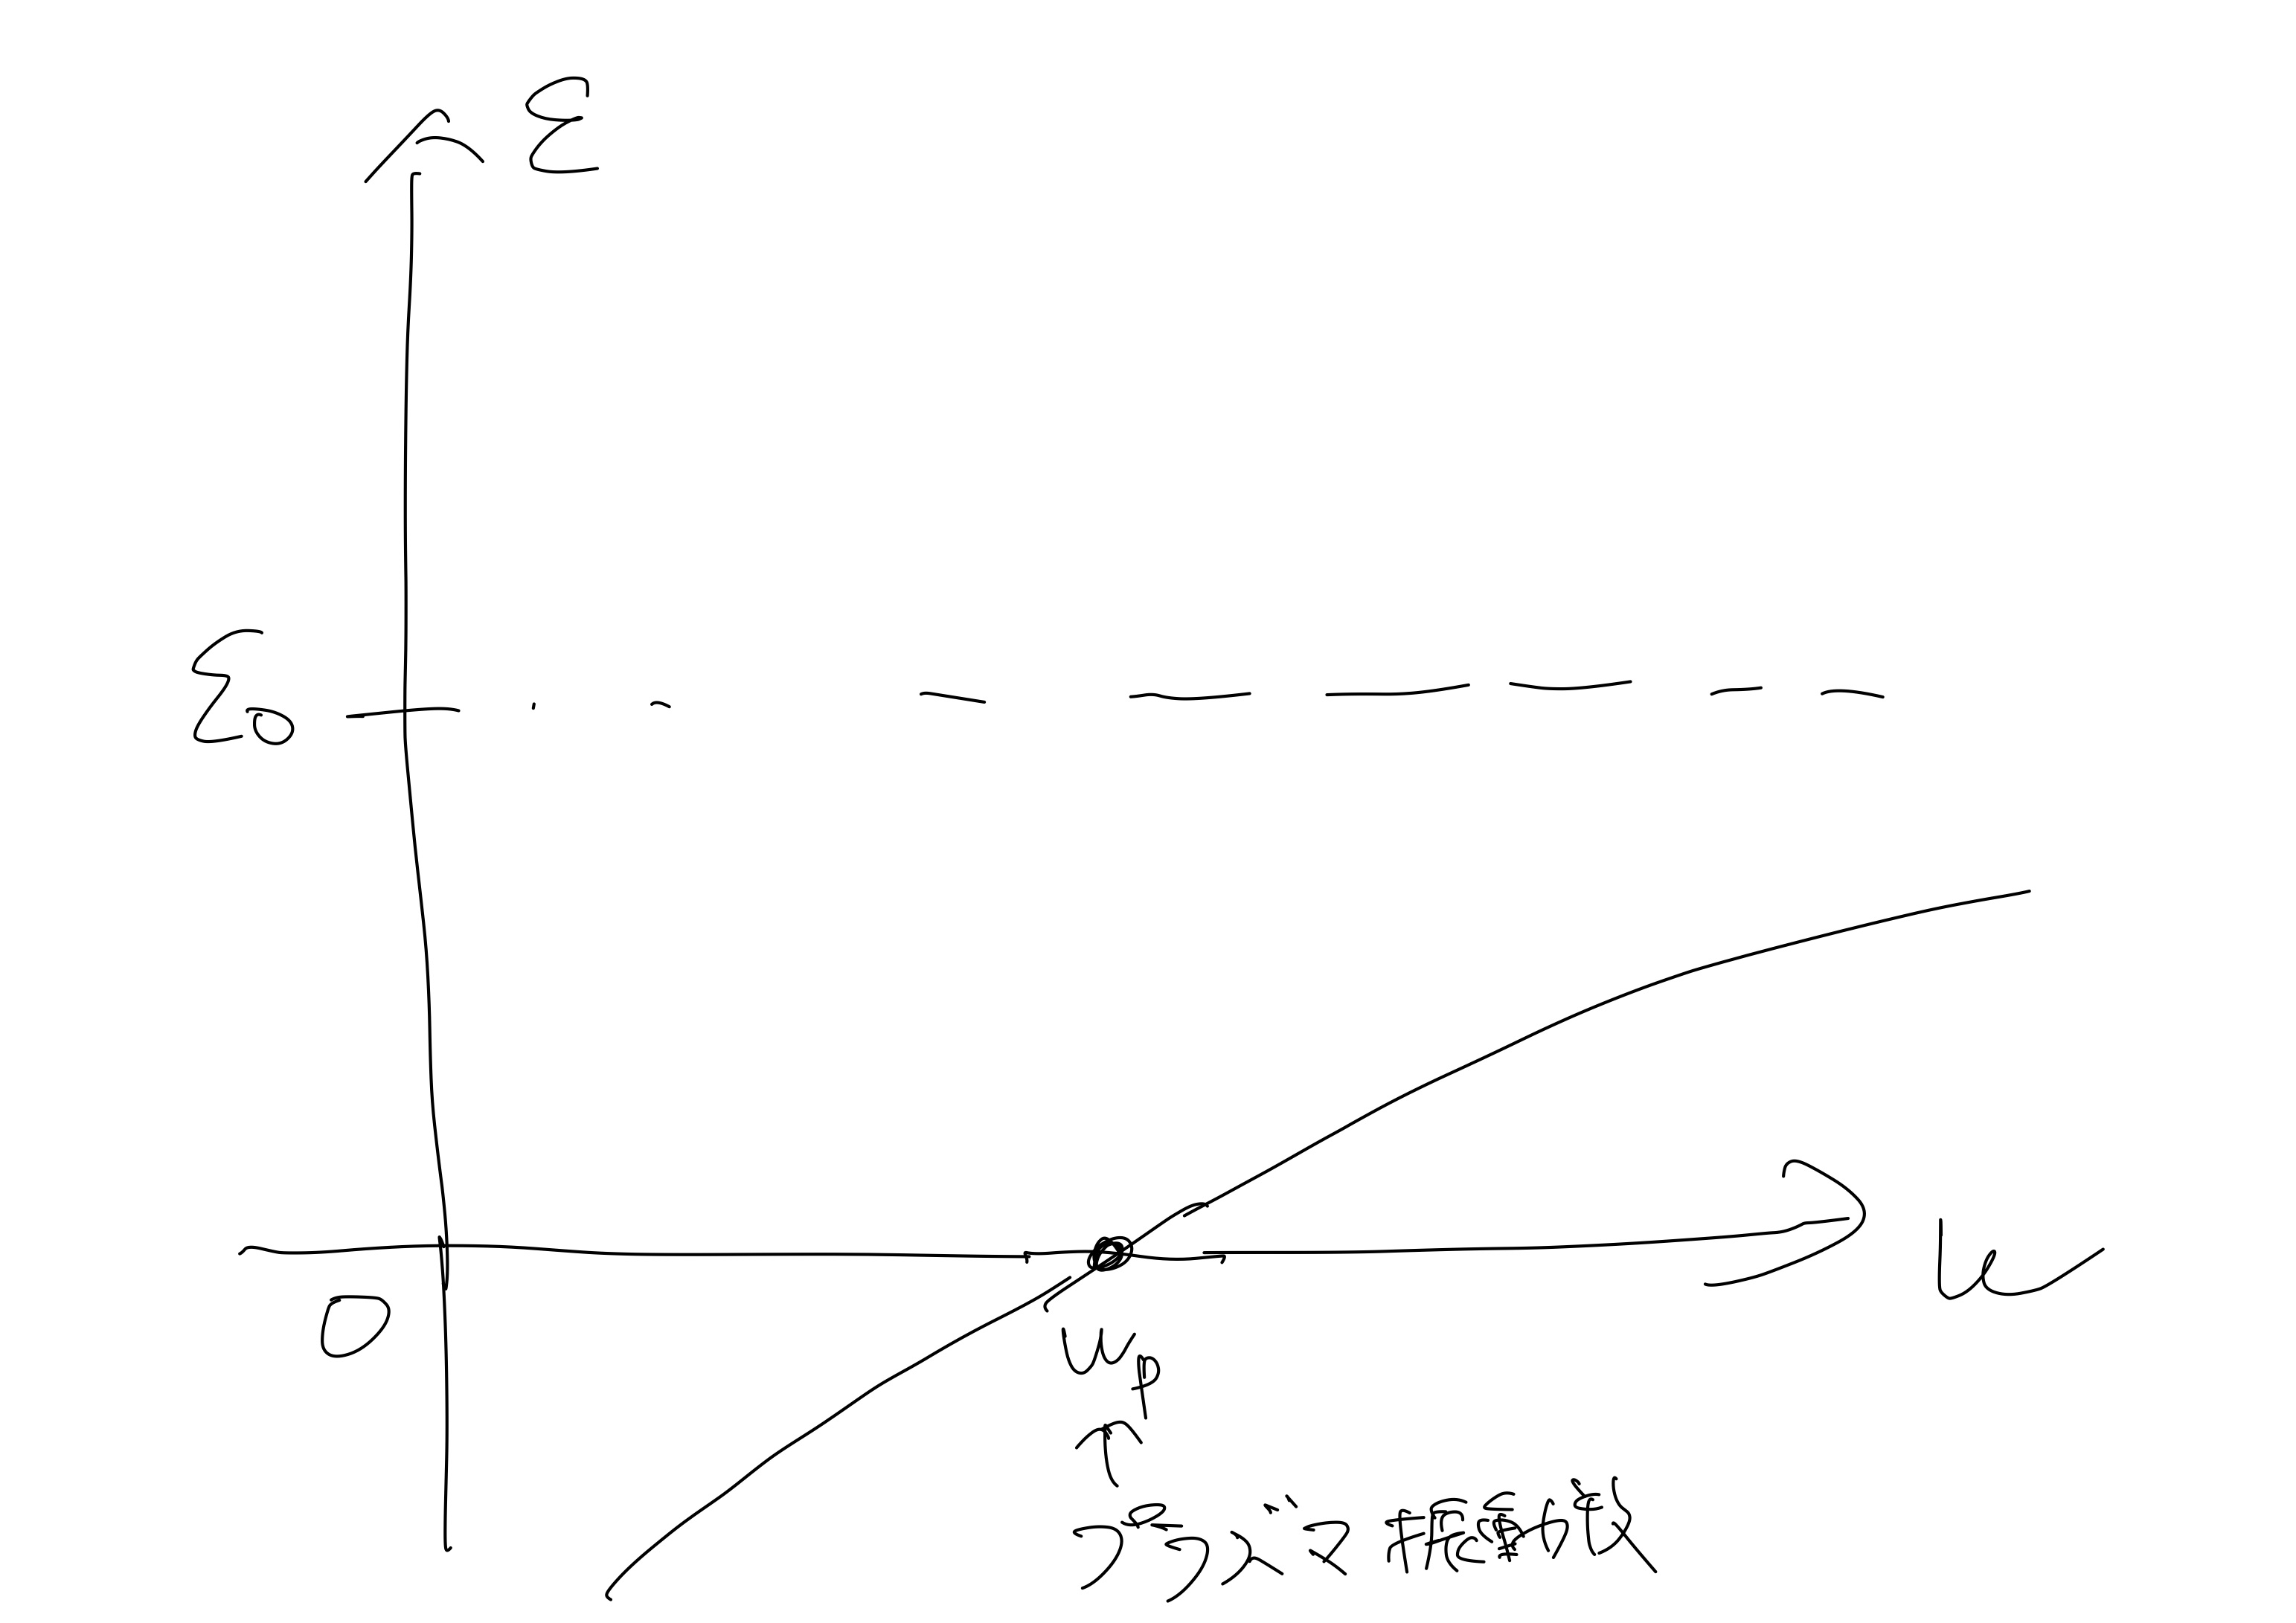
\includegraphics[width=0.5\textwidth]{fig1/Fig-3.jpg}
	\caption{fig1/Fig-3.jpg}
	\label{fig:fig1-Fig-3-jpg}
\end{figure}

つづいて磁性について
まず磁性という性質は古典的には説明できない。
この磁気モーメントの発生する原因がスピン角運動量でありこれは古典的には説明できない。
古典的なモデルでは磁気モーメントがなくなるということがわかる( なんかそういう定理があるはず)。
磁性はほとんどの物質ではでない。普通磁石になるような物質というのは希土類と遷移金属が含まれている。これ以外の物質で磁石になるやつは今までにない。

\[
H=-\sum_{<i,j>}^{}J_{ij} \bm{S}_i\cdot \bm{S}_j
.\] 
$J_{ij}$ を正確に計算するというのは難しい。
波動関数の重なりに起因する相互作用であり、隣り合ったところからちょっとでも離れると考えなくて良くなるので隣り合った奴らだけ考える。
こうやって考えたときに$J<0,>0$ の場合がある。
これによって強磁性か反強磁性かがきまる。
これを簡単に考えるために分子場理論とか平均場理論とかを考えていく。
これは周りからの相互作用を自己無同着な形で方程式を解いていくことによって磁化とかを出していく。

また伝導電子が示す磁性というものありこれはパウリ譲二性とかランダウ判事性がある。これは電子がスピン、ランダウ判事性は電子の輝度運動からでるものである。
これは理論亭な取扱はすが置く難しいがまだちゃんとわかっていない。
例えば鉄とかニッケルが磁石になるのは格子点に止まっているきょくざいしたやつが磁石になるだけでは説明できなくてこれを伝導電子にも拡張するのはわかっていない。これを現象論的に認めて議論を進めていく。


最後に超電導の基本的な事柄について熱力学と統計力学で考える。
\begin{figure}[H]
	\centering
	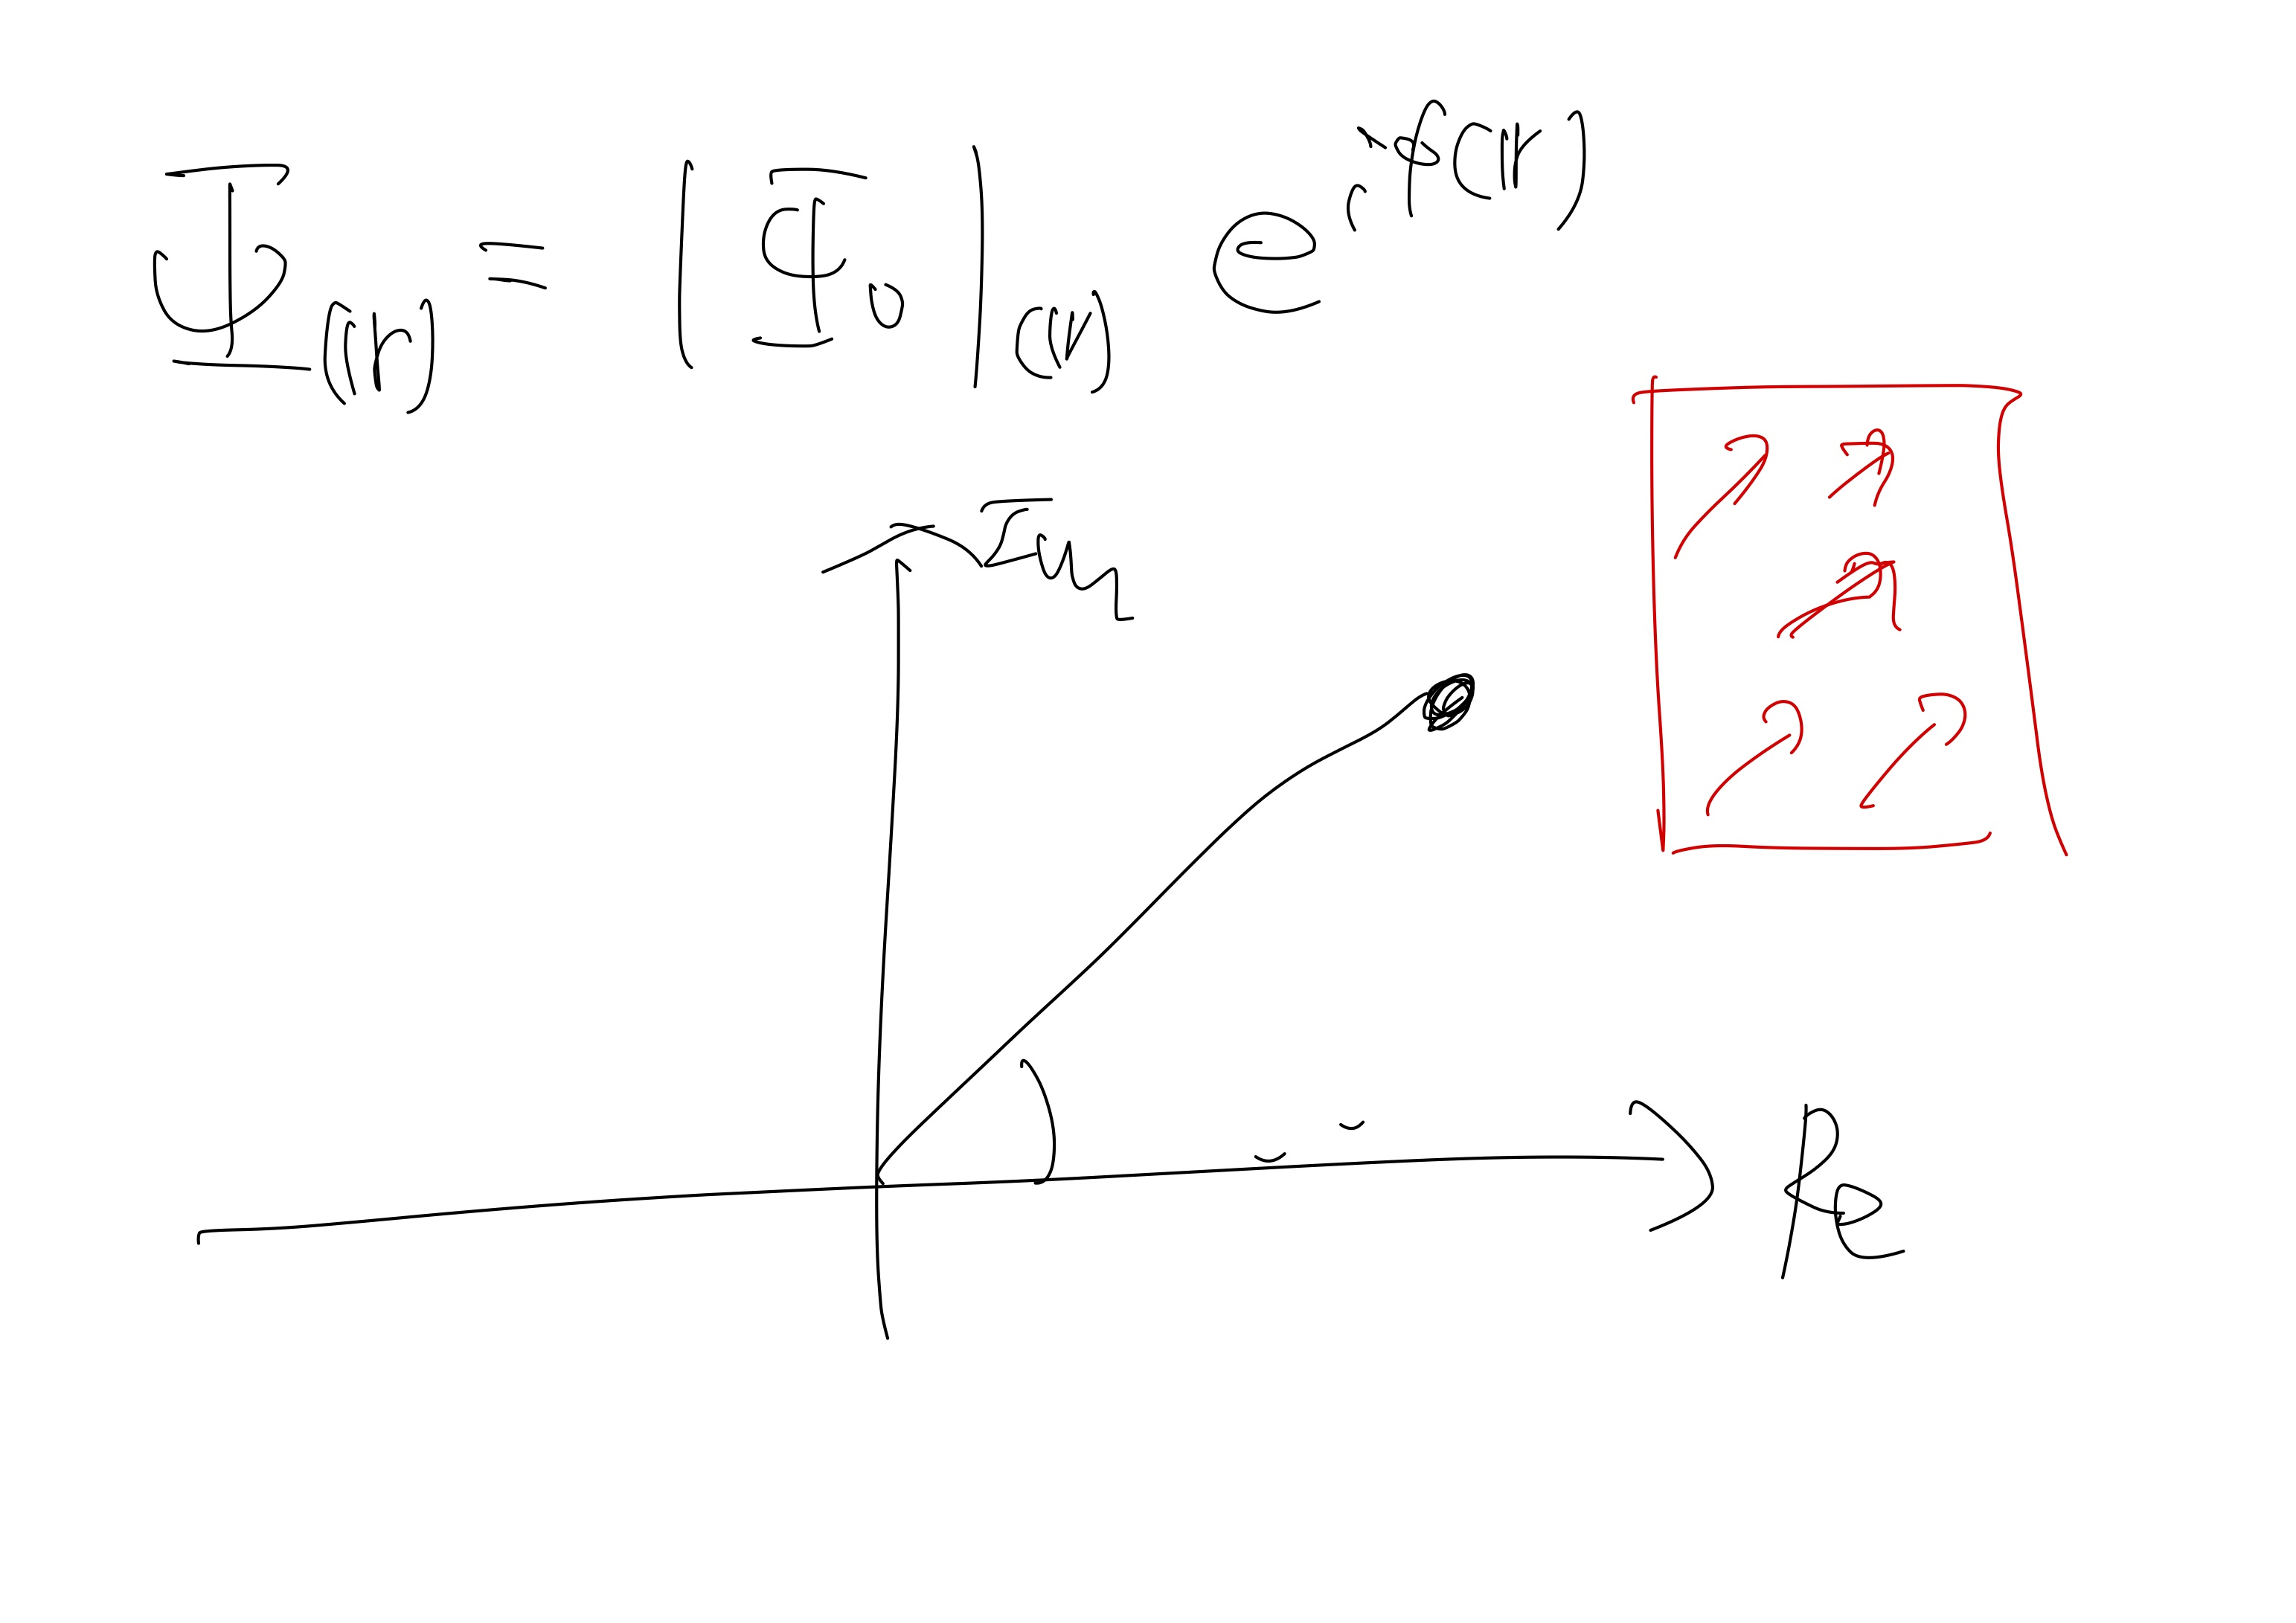
\includegraphics[width=0.5\textwidth]{fig1/Fig-4.jpg}
	\caption{fig1/Fig-4.jpg}
	\label{fig:fig1-Fig-4-jpg}
\end{figure}
ちょうでんどうがある秩序を持ったものとして考えて秩序パラメータを導入する。これは複素数である。
例えば磁性において臨海温度よりも低温ではスピンが同じ方向を向いている。このときにこれを巨視的な一つの磁化とかんがえると、これは時期秩序を表すへんすうになっていて秩序変数とか秩序パラメ多という。
そうすると磁化がゼロでないときとゼロのときという状態が考えられて,

超伝導体の中には複素空間があってバラバラな向きを向いて賞味ゼロだったのが超伝導になるとこの矢印が揃ってしまうということがわかる。

磁性体の中でもXY模型と超電導はと等価である。

ここだけではまだ不十分でBCS理論がなきゃだめ。これは電子がフェルミ球を作っている不安定になると原子は束縛状態をとったほうが安定する。つまり対を作ろうとする。これがBCS理論。

あとは授業で扱わないやるもあるが、強相関とかトポロジカル物質とかは扱わない。近藤効果も扱わない。


2022/10/13/num2
\section{屈折率とはなにか}

\begin{figure}[H]
	\centering
	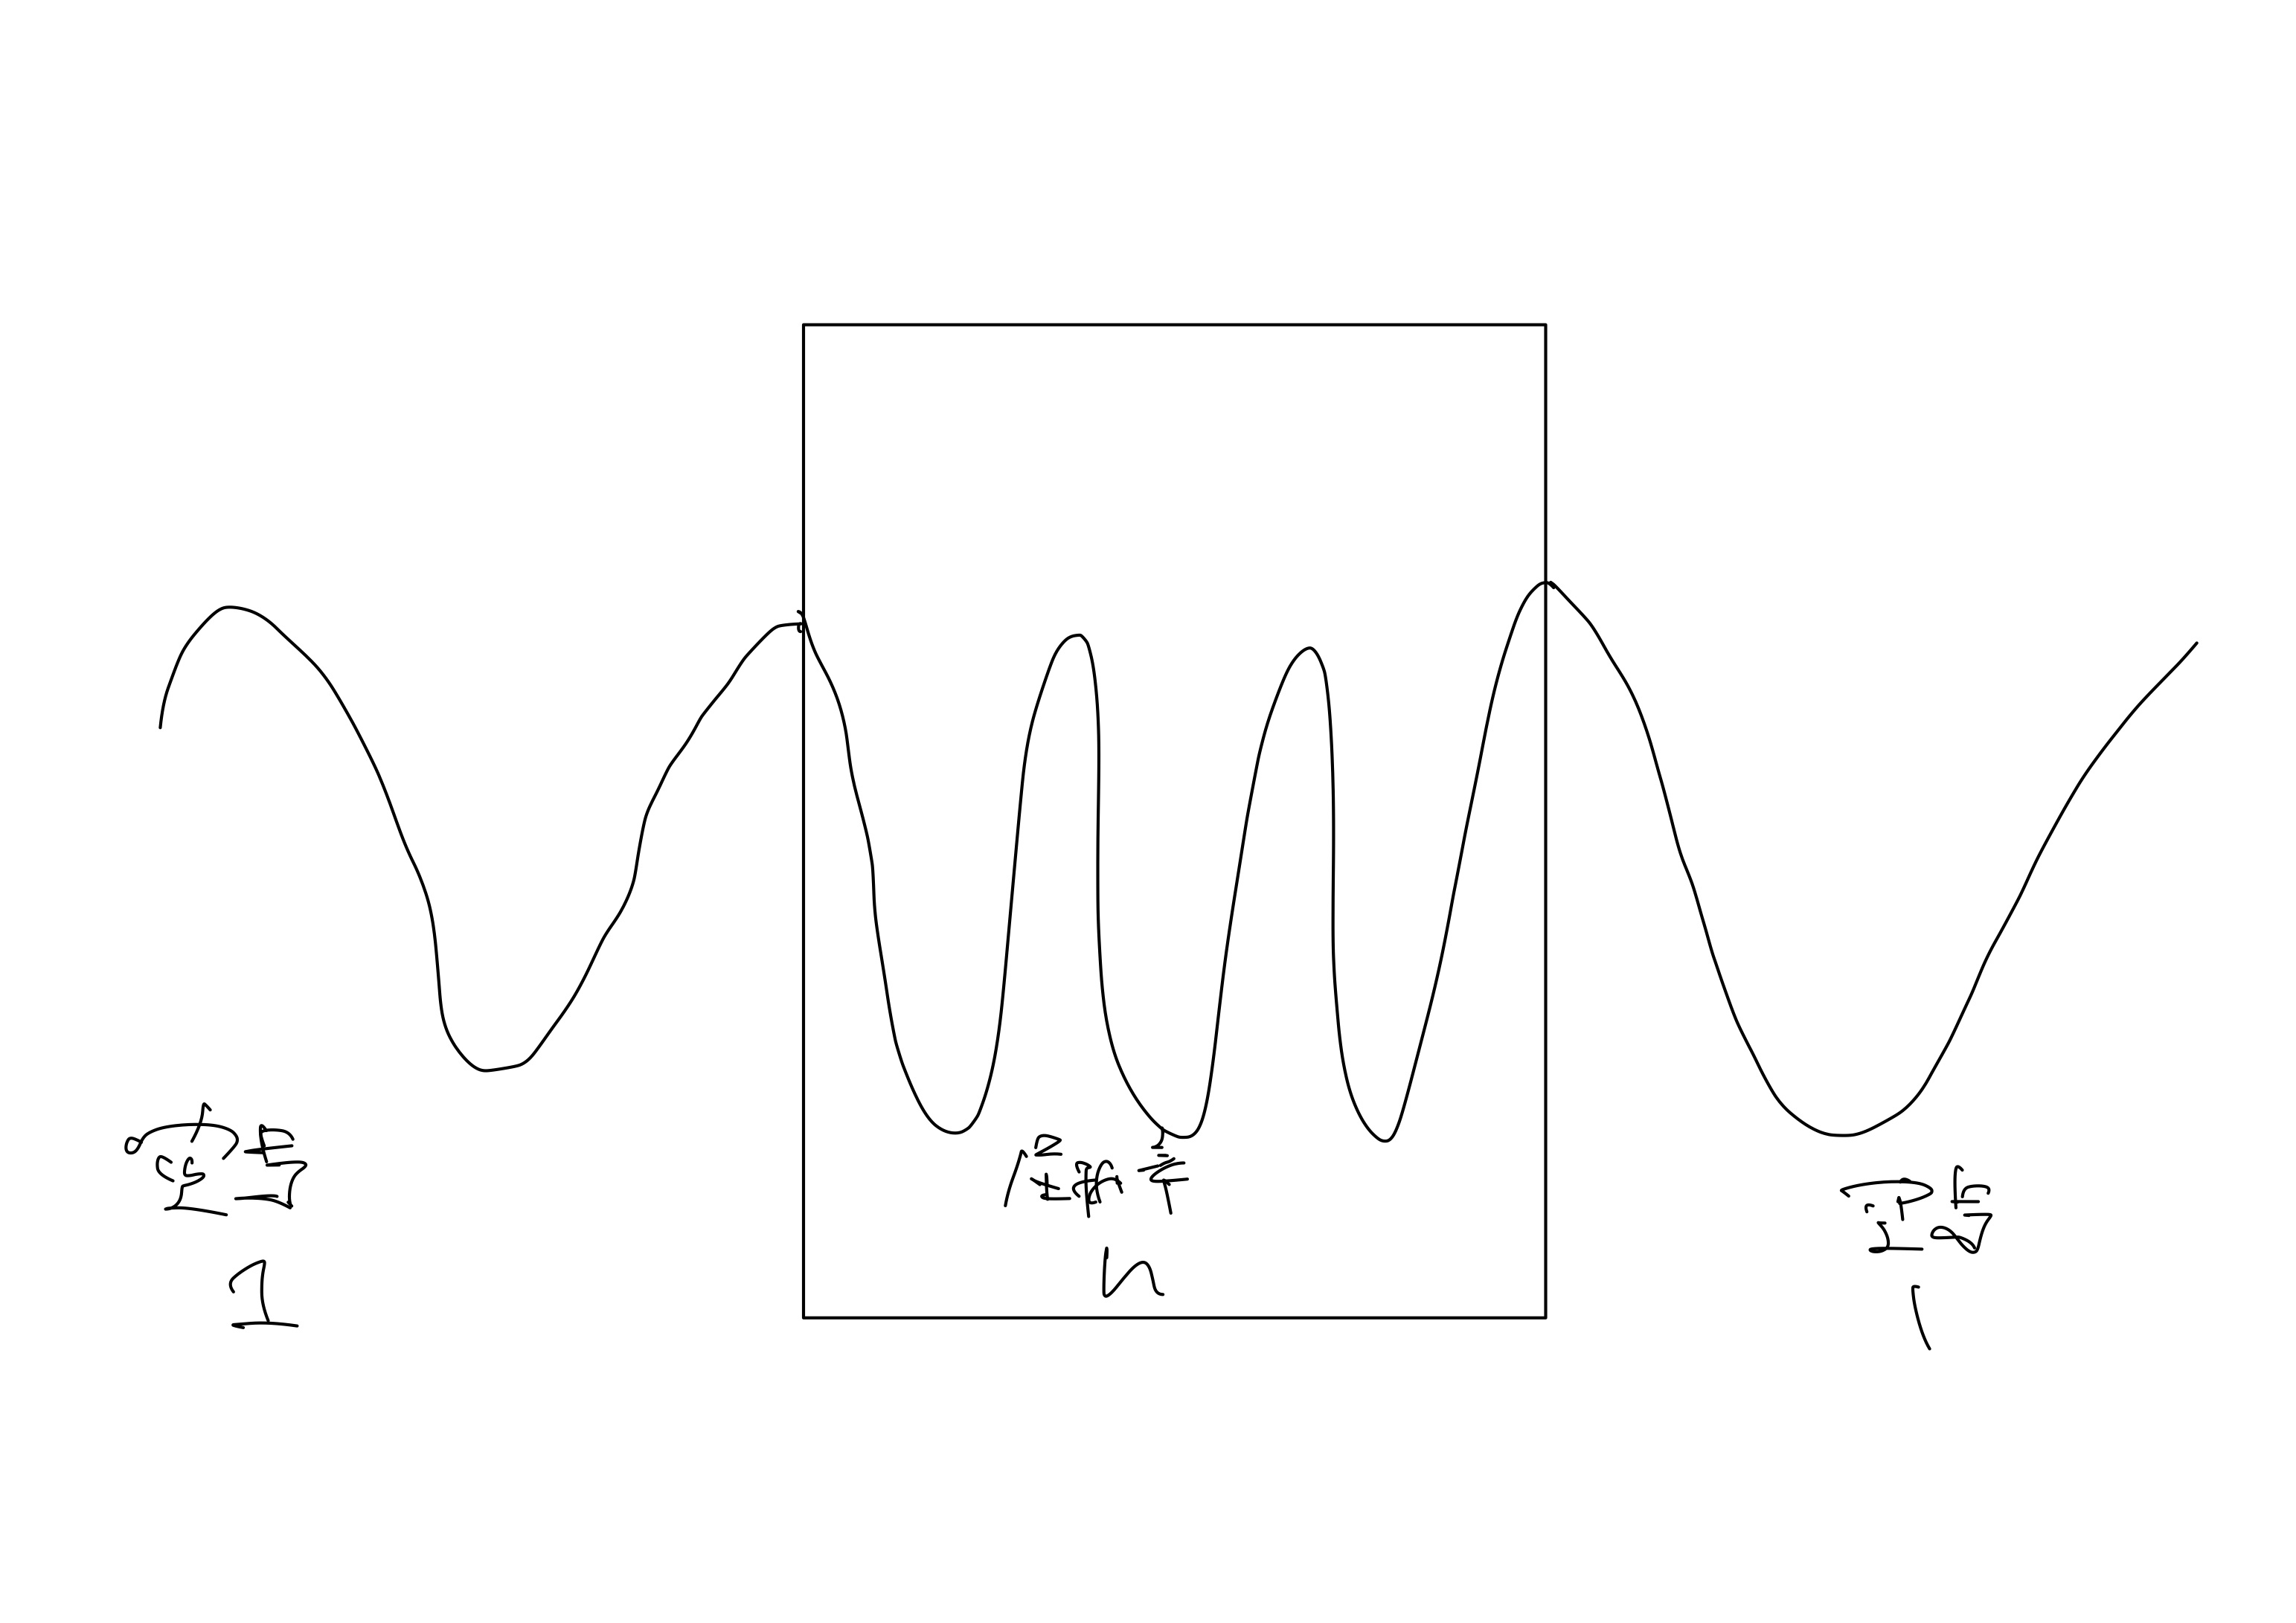
\includegraphics[width=0.3\textwidth]{fig2/Fig-2.jpg}
	%\caption{}
	\label{fig:fig2-Fig-2-jpg}
\end{figure}
光が屈折率$n$ の媒質に入ると波長が$1 /n$ になる。
\[
\lambda\to \frac{\lambda}{n}
.\] 
速さが光速の$1 /n$ で進むように見える
\[
c\to \frac{c}{n}
.\] 
様々な物質の屈折率 ($\lambda=\SI{0.5893}{\micro m}$)
\begin{table}[H]
	\centering
	\caption{様々な物質の屈折率 ($\lambda=\SI{0.5893}{\micro m}$)}
	\label{tab:2-1}
	\begin{tabular}{ccc}\hline
	 &$n$ &密度($\si{g.cm^-3}$)\\ \hline
	空気&1.000292&$1.3\times 10^{-3}$\\
	水&1.333&$\sim 1$\\
	ガラス&$\sim 1.5$&$2.2\sim 2.6$\\
	ダイヤモンド&2.42&3.51\\ \hline
	\end{tabular}
\end{table}
密度が大きいほど屈折率が大きい。
密度と$n$ の関係。
なぜ光の速さが見かけ上$c /n$ になるのか。なぜ波長が短くなるのか。
これを簡単なモデルで考える。
\subsection{物質中の光の(見かけ上の)速さの意味}
\begin{figure}[H]
	\centering
	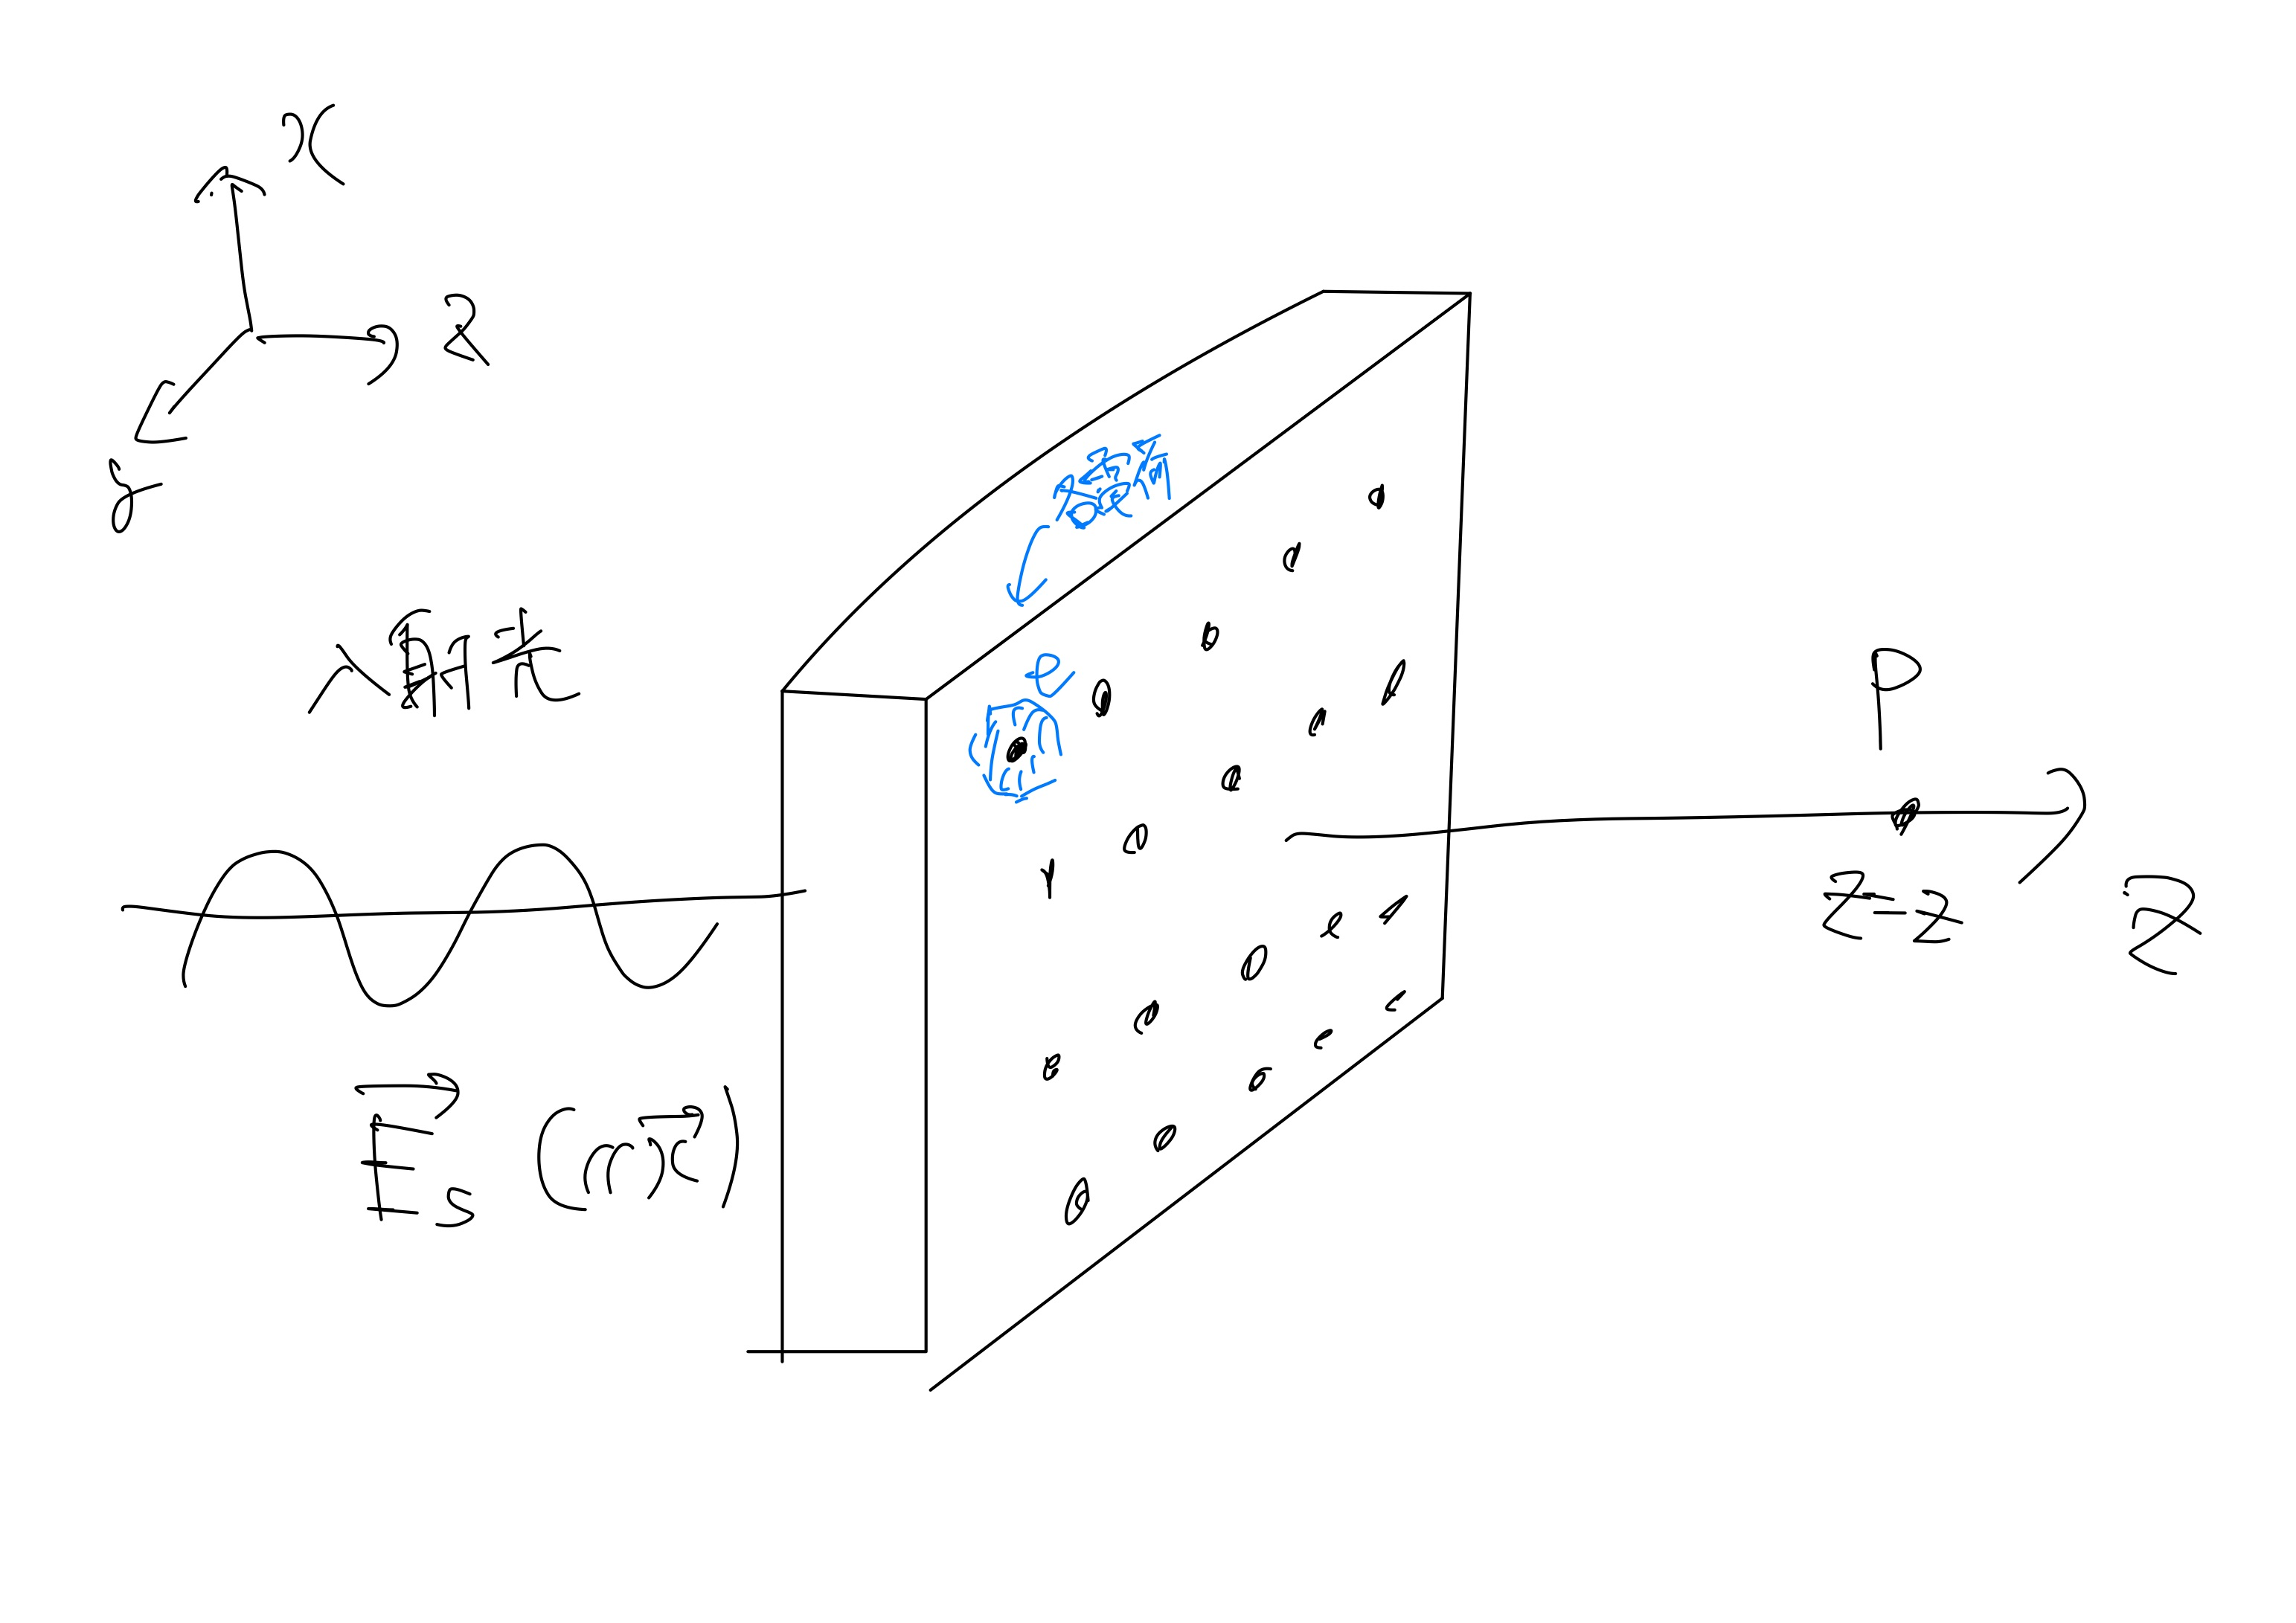
\includegraphics[width=0.5\textwidth]{fig2/Fig-3.jpg}
	%\caption{}
	\label{fig:fig2-Fig-3-jpg}
\end{figure}
P点での電場は
\begin{tcolorbox}[colback=green!10!white]
\begin{equation}
\label{eq:2-1}
\bm{E}=\bm{E}_s+\sum_{\text{物質中の全電荷}}^{} \bm{E}_{\text{各電荷}}=\bm{E}_s+\bm{E}_a
.\end{equation}
\end{tcolorbox}
\eqref{eq:2-1}の第二項は二次光$\bm{E}_a$ と書かれる。

ここで
\begin{align*}
	\label{eq:2-2}
	\bm{E}_s&= \bm{E}_0 \cos (\omega t-kz) \\
	&= \bm{E}_0 \cos \omega(t-\frac{z}{c}) \\
	&\to  \bm{E}_0e^{i\omega(t-\frac{z}{c})} 
	\stepcounter{equation}\tag{\theequation} 
.\end{align*}
ここで$\bm{E}_a$ の起源はなにか考える。
\begin{figure}[H]
	\centering
	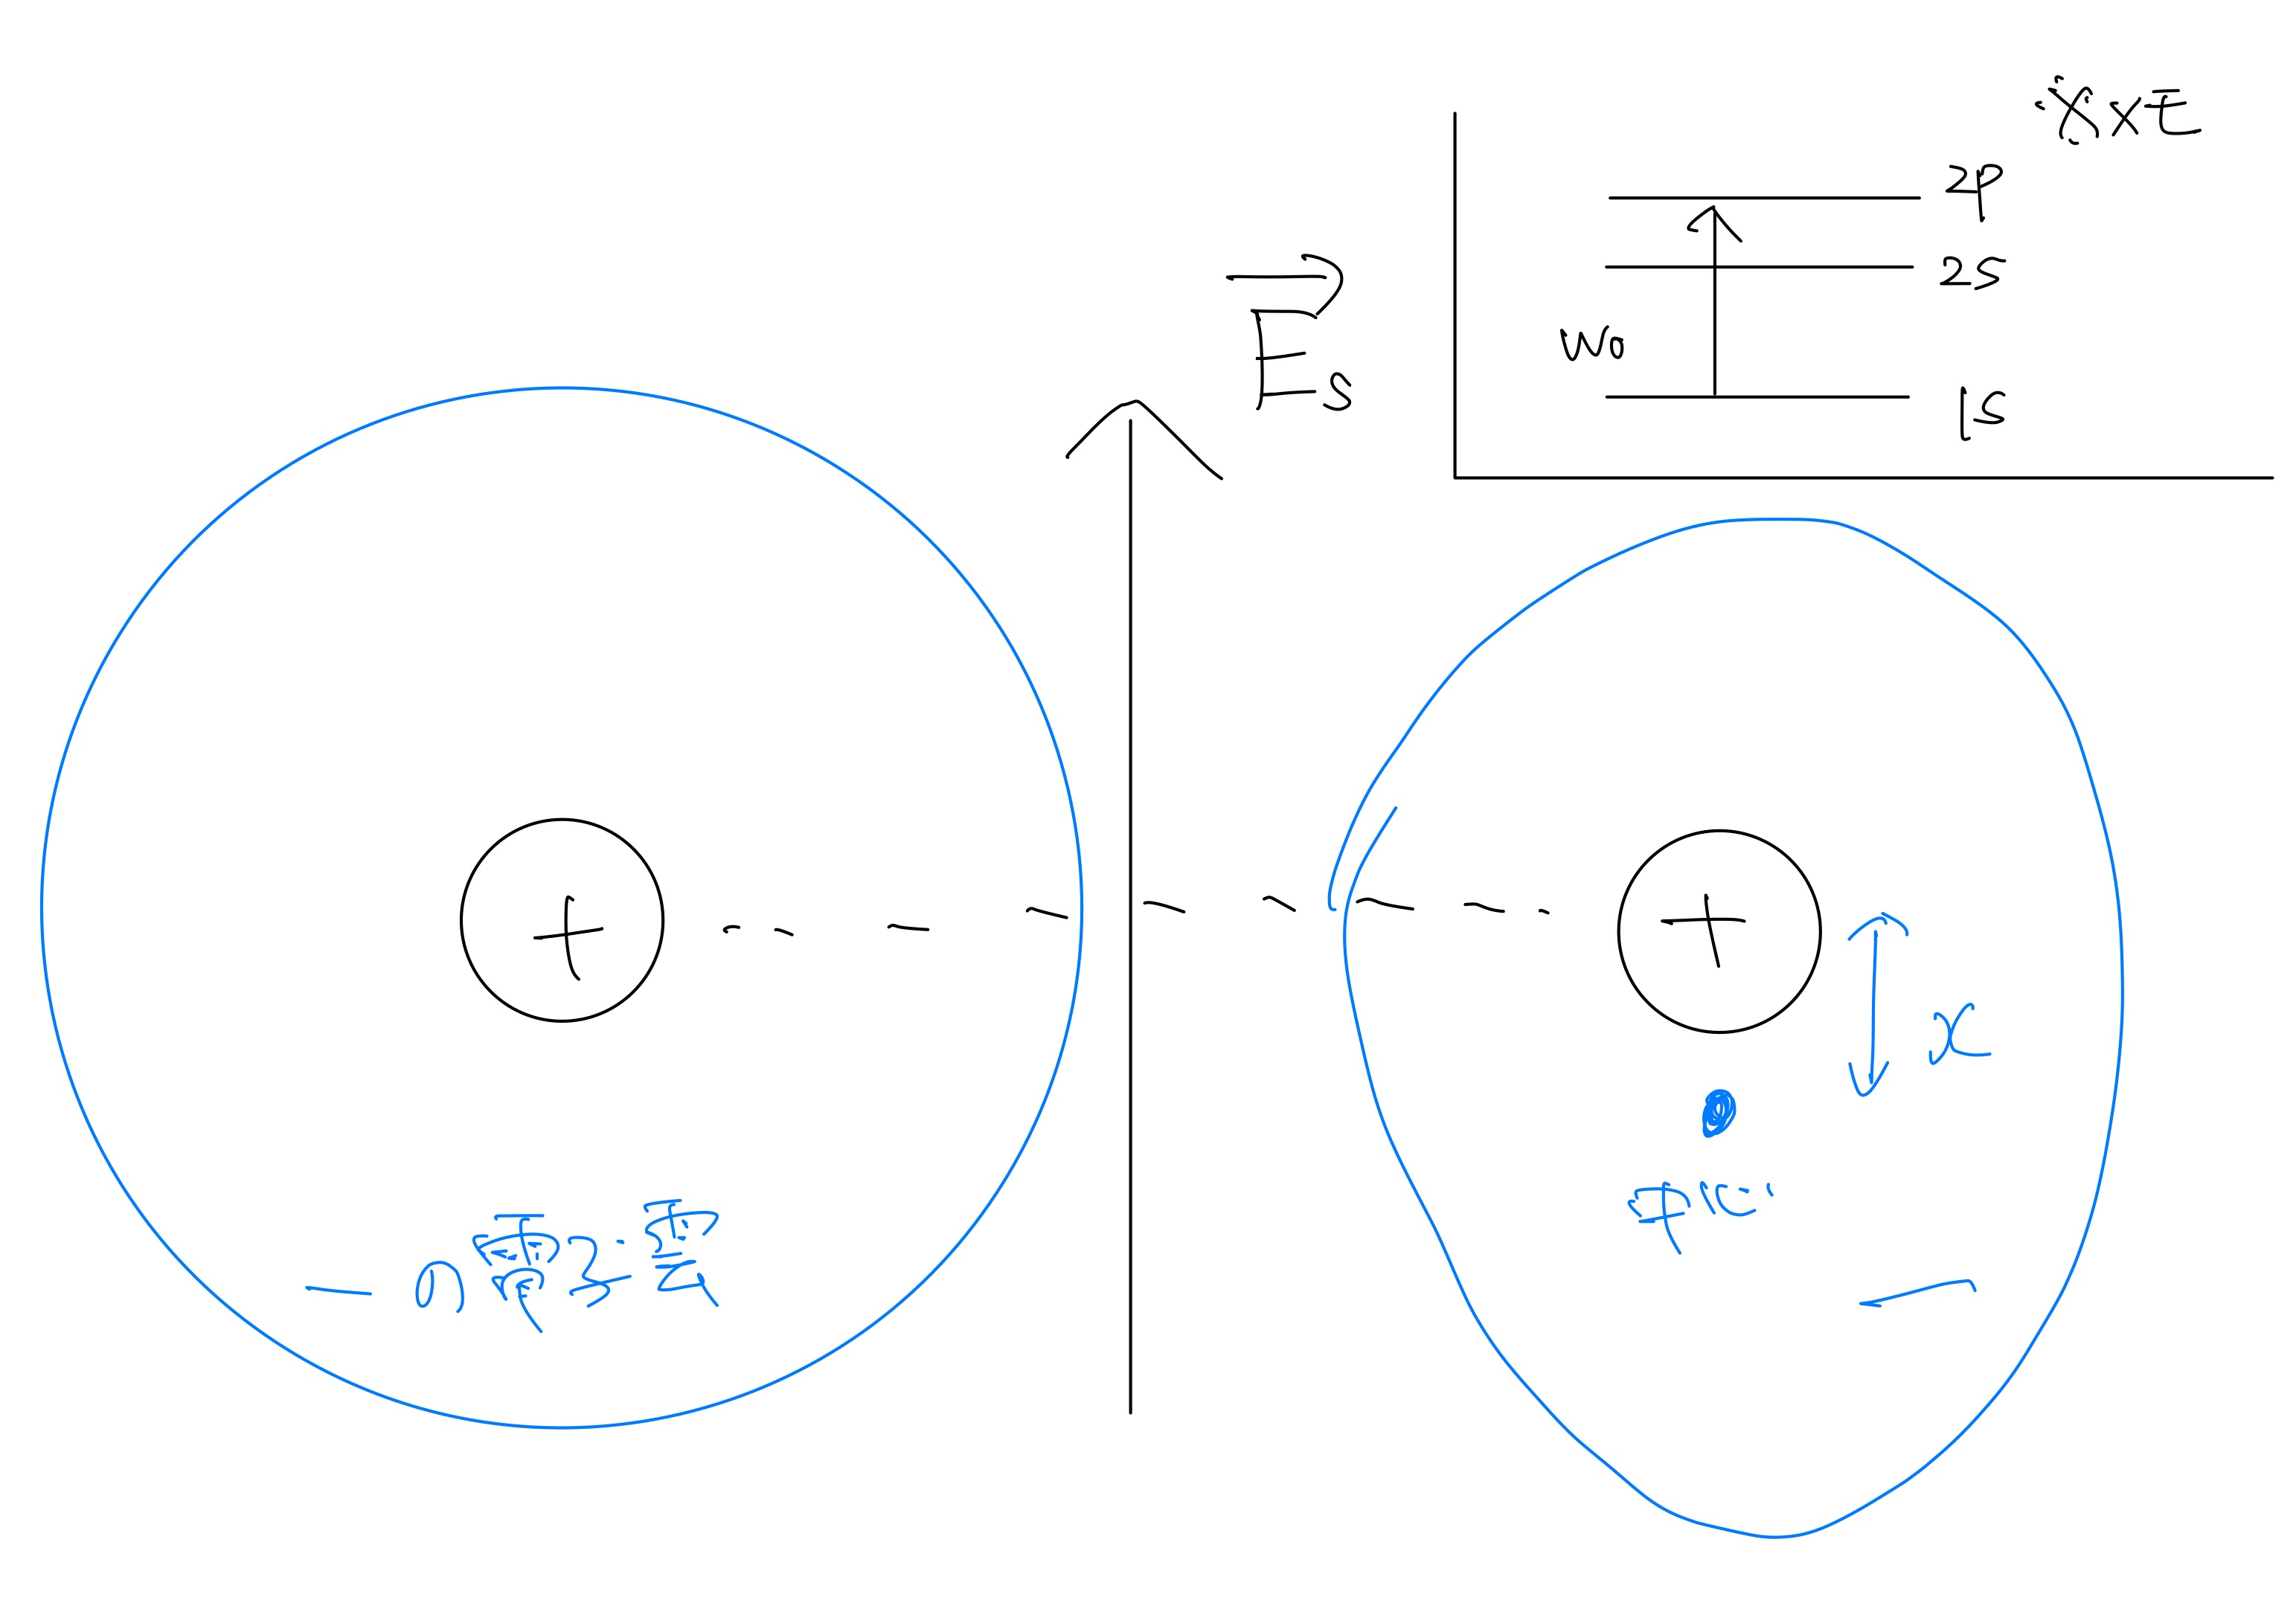
\includegraphics[width=0.5\textwidth]{fig2/Fig-4.jpg}
	%\caption{}
	\label{fig:fig2-Fig-4-jpg}
\end{figure}
光電場によって原子の中の電子が強制振動するとかんがえる。(固有振動数$\omega_0$)
これは\textcolor{red}{ローレンツ振動子}と呼ばれる。
一応この振動数$\omega_0$ は 1sから2pへの遷移振動数に対応する。

\begin{equation}
\label{eq:2-3}
m_e \left( \frac{d^2x}{dt^2}+2\gamma \frac{dx}{dt}+\omega_0^2x \right) =-eE_s
.\end{equation}
簡単のため左辺第二項の摩擦項はゼロとする。

量子力学との対応を考えると\eqref{eq:2-3}の固有振動数$\omega_0$は
光による量子状態間遷移に対応する。

\eqref{eq:2-3}に\eqref{eq:2-2}を代入すると
\begin{equation}
\label{eq:2-4}
	x(t)=\frac{-eE_0}{m(\omega_0^2-\omega^2)}e^{i\omega t}:=-A(\omega)e^{i\omega t}
.\end{equation}
\eqref{eq:2-4}を二階微分して
\begin{equation}
\label{eq:2-5}
	\frac{d^2x}{dt^2}=A(\omega)\omega^2e^{i\omega t}
.\end{equation}
双極子モーメントの振動によって電磁波の放射が起こる。
十分遠方での解は
\begin{equation}
\label{eq:2-6}
E_\text{各電荷} \sim \frac{eA(\omega)\omega^2}{4\pi\varepsilon_0c^2} \frac{e^{i\omega(t-\frac{r}{c})}}{r}
.\end{equation}
重要なのは指数の方の部分で点$P$ では電場が遅れているということである。
\begin{figure}[H]
	\centering
	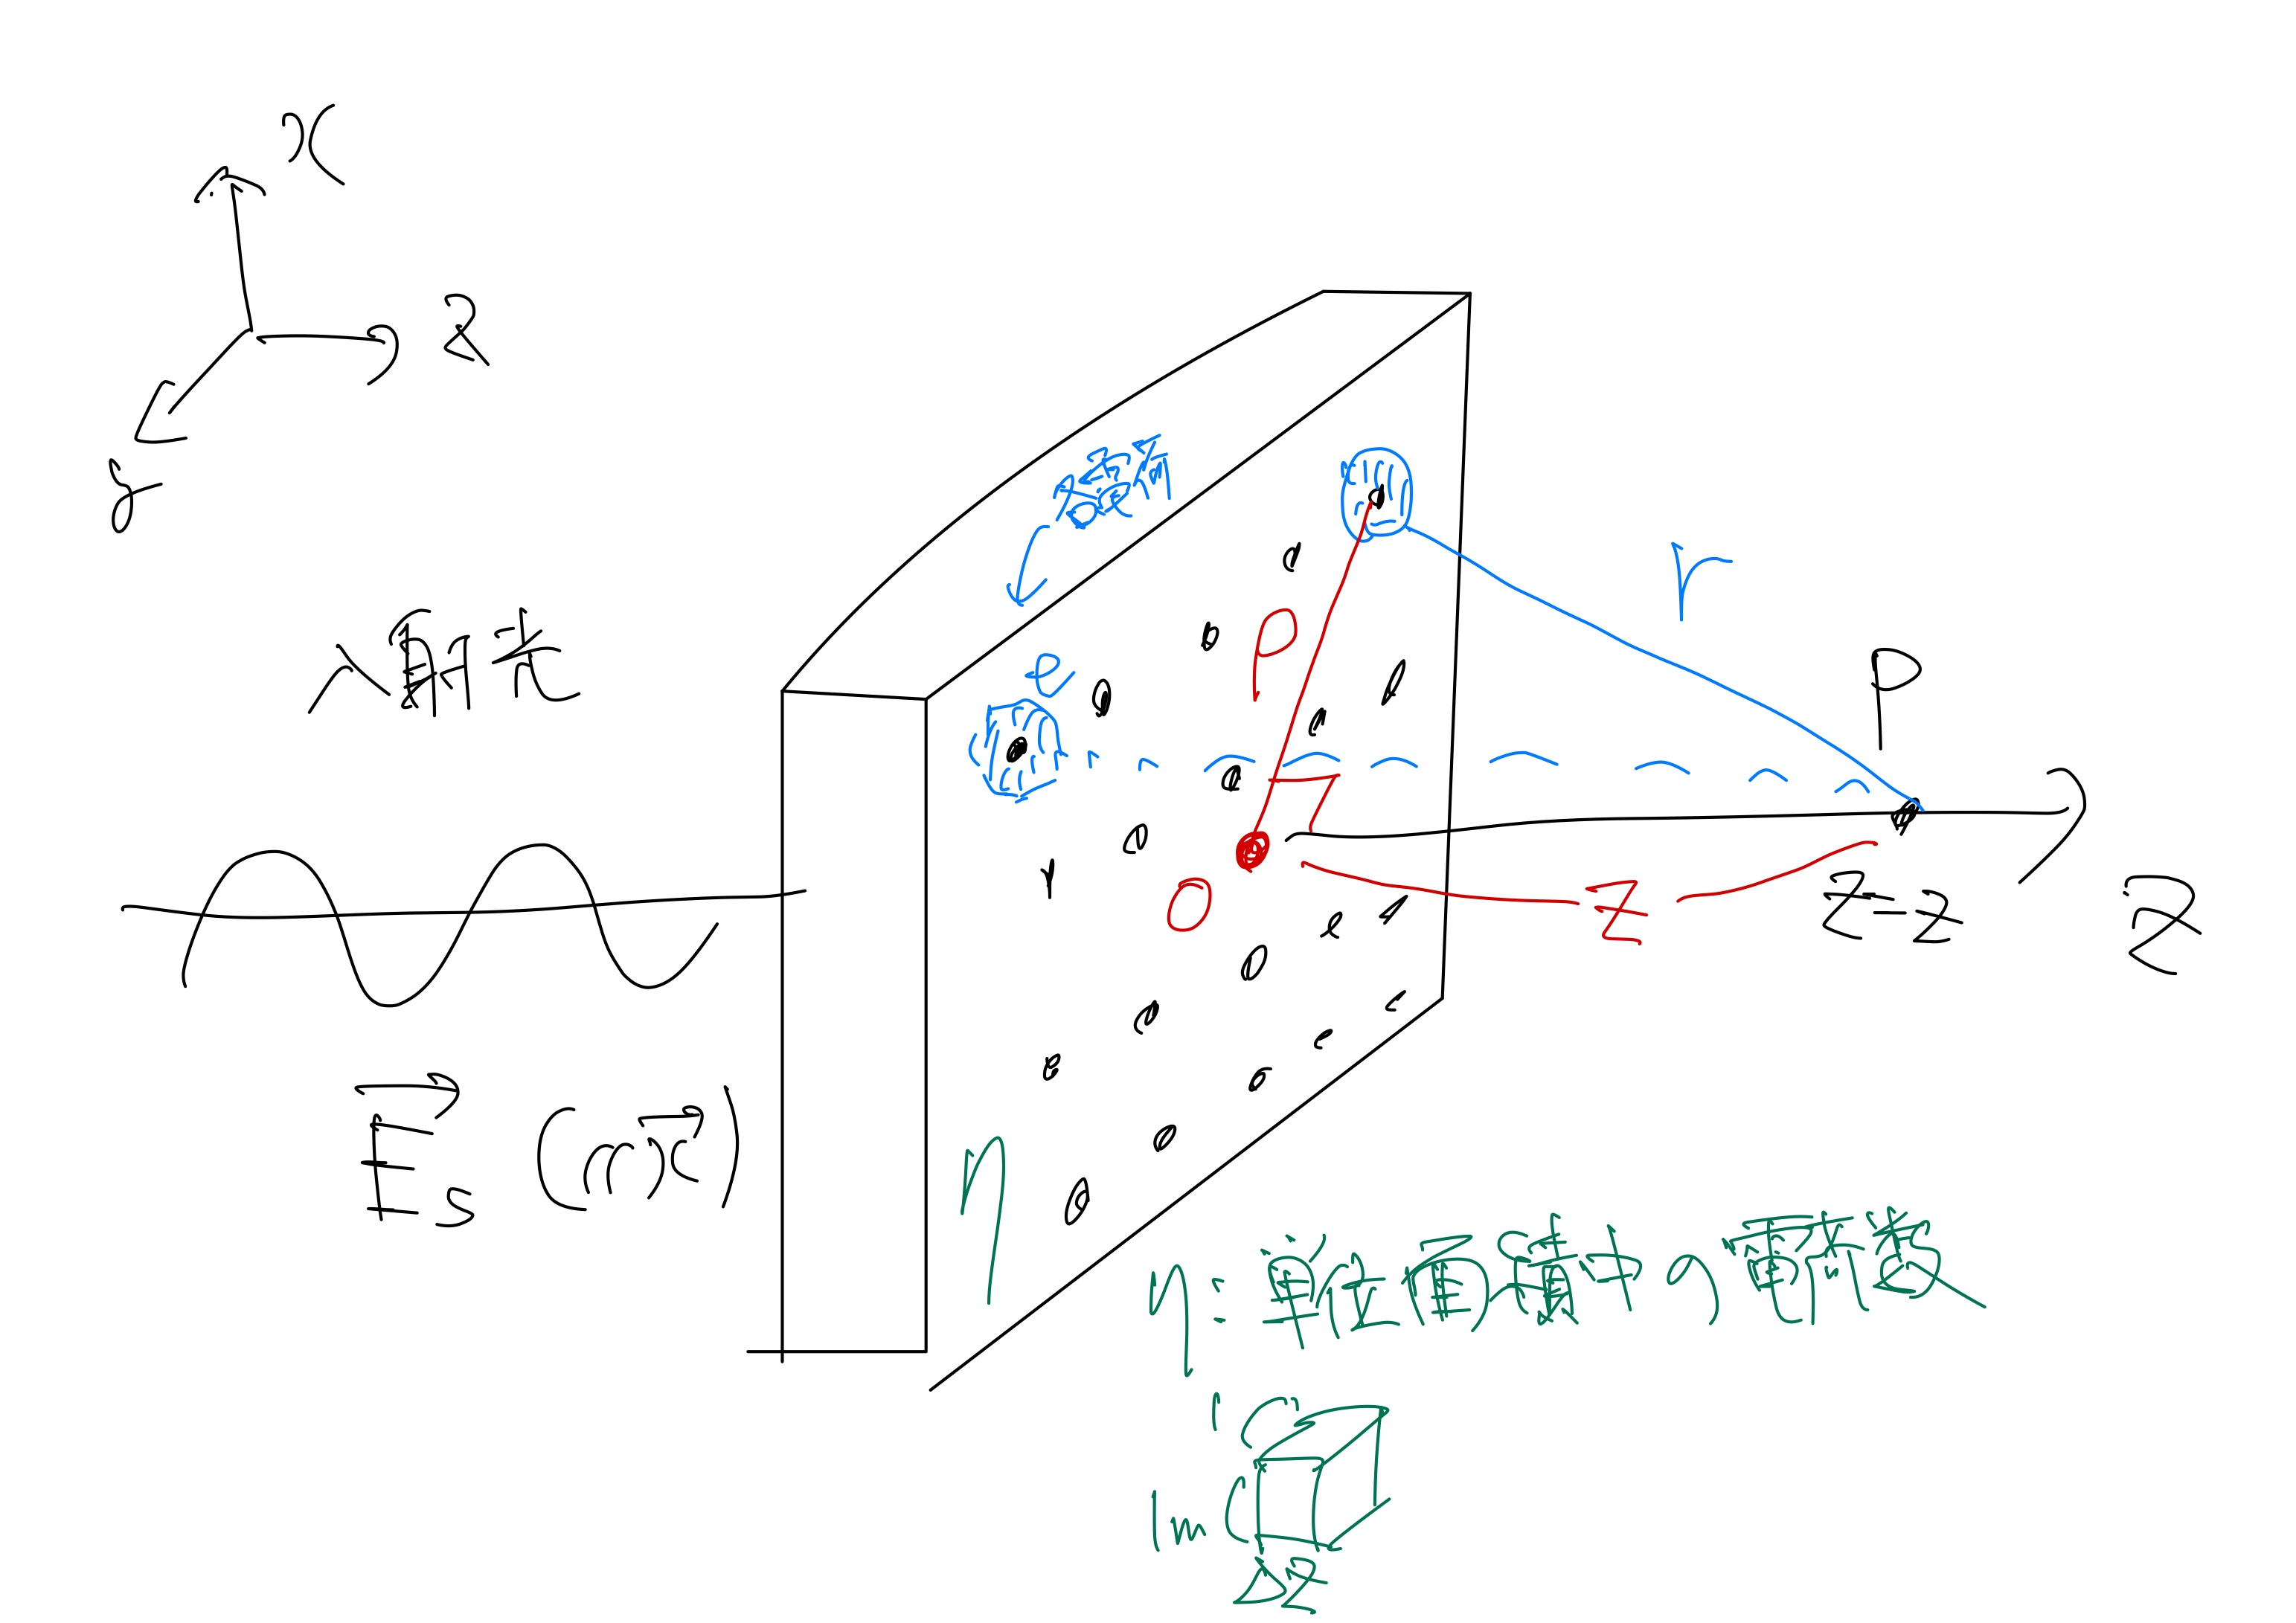
\includegraphics[width=0.5\textwidth]{fig2/Fig-5.jpg}
	%\caption{}
	\label{fig:fig2-Fig-5-jpg}
\end{figure}
\[
r^2=\rho^2+z^2
.\] 
\[
2r dr=2\rho d\rho 
.\] 
物質中の全電荷の寄与を足し合わせると
\begin{equation}
\label{eq:2-7}
	E_a=\int_{0}^{\infty} \frac{eA(\omega)\omega^2}{4\pi\varepsilon_0c^2}\frac{e^{i\omega(t-\frac{r}{c})}}{r}\eta 2\pi \rho d\rho 
.\end{equation}
$E_a$ の積分は
\begin{equation}
\label{eq:2-8}
\int_{0}^{\infty} \frac{e^{\frac{-i\omega r}{c}}}{r}\rho d\rho = \int_{z}^{\infty} e^{-i \frac{\omega}{c}r}dr  =+\frac{c}{i\omega}e^{-i \frac{\omega}{c}z}
.\end{equation}
を計算すれば良い。
興味があれば動画の53:28みろ

したがって最終結果は
\begin{equation}
\label{eq:2-9}
	E_a=(-i)\frac{e}{2\varepsilon_0}A(\omega) \frac{\omega}{c}\eta\cdot  e^{i\omega(t-\frac{z}{c})}:=(-i)E_0B(\omega)e^{i\omega(t-\frac{z}{c})}
.\end{equation}
\eqref{eq:2-1}より点Pでの電場(の$x$成分)は
\[
E=E_s+E_a\sim E_0e^{i\omega(t-\frac{z}{c})}+E_0B(\omega)\cdot (-i)e^{i\omega(t-\frac{z}{c})}=E_0\left\{ 1-iB(\omega) \right\} e^{i\omega(t-\frac{z}{c})}
.\] 
ここで以下の近似
\[
e^{-ix}\sim 1-ix\quad (x\ll 1)
.\] 
を用いると
\begin{equation}
\label{eq:2-10}
E(t,z)\sim E_0e^{i\omega(t-\frac{z}{c}-\frac{B(\omega)}{\omega})}
.\end{equation}
ここで指数の肩の$-\frac{B(\omega)}{\omega}$ が
二次項による見かけ上の光の遅れに対応する。
\begin{figure}[H]
	\centering
	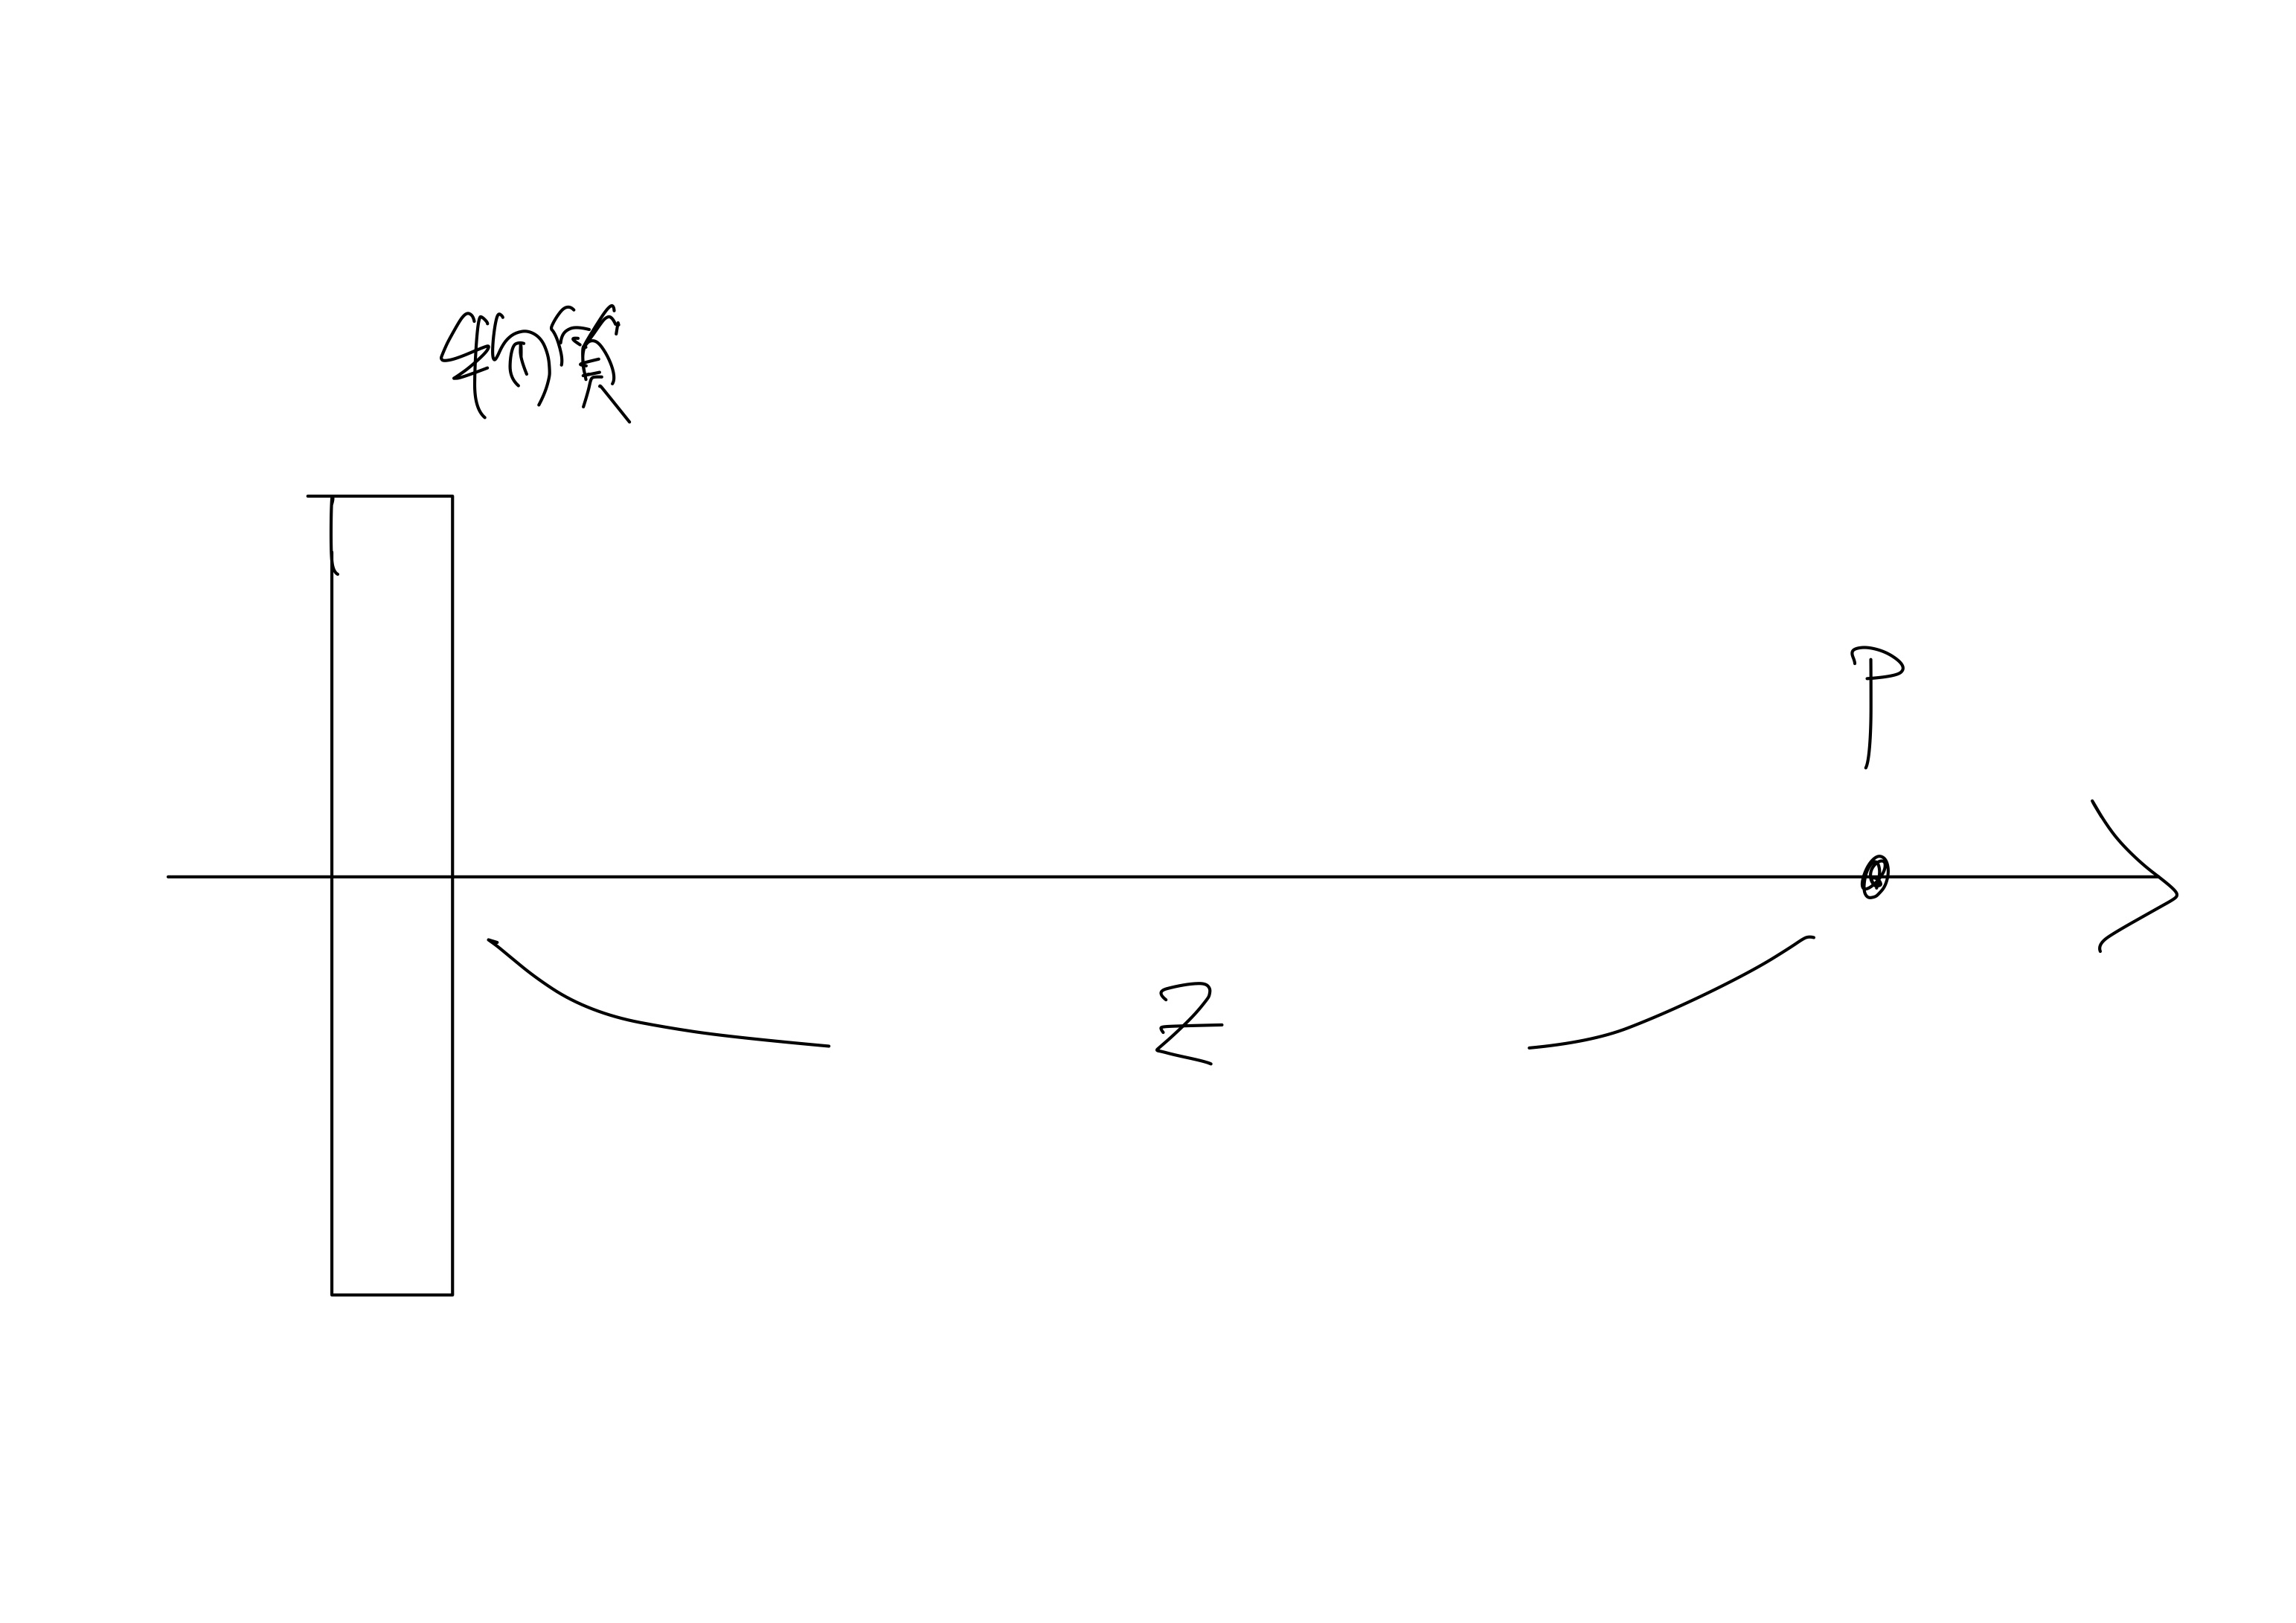
\includegraphics[width=0.4\textwidth]{fig2/Fig-6.jpg}
	%\caption{}
	\label{fig:fig2-Fig-6-jpg}
\end{figure}
例えば簡単のため$z= \frac{2\pi c}{\omega}\cdot N $ のとき
\begin{equation}
\label{eq:2-11}
	E(t)=E_0e^{i\omega(t-\frac{B(\omega)}{\omega})}
.\end{equation}
\begin{figure}[H]
	\centering
	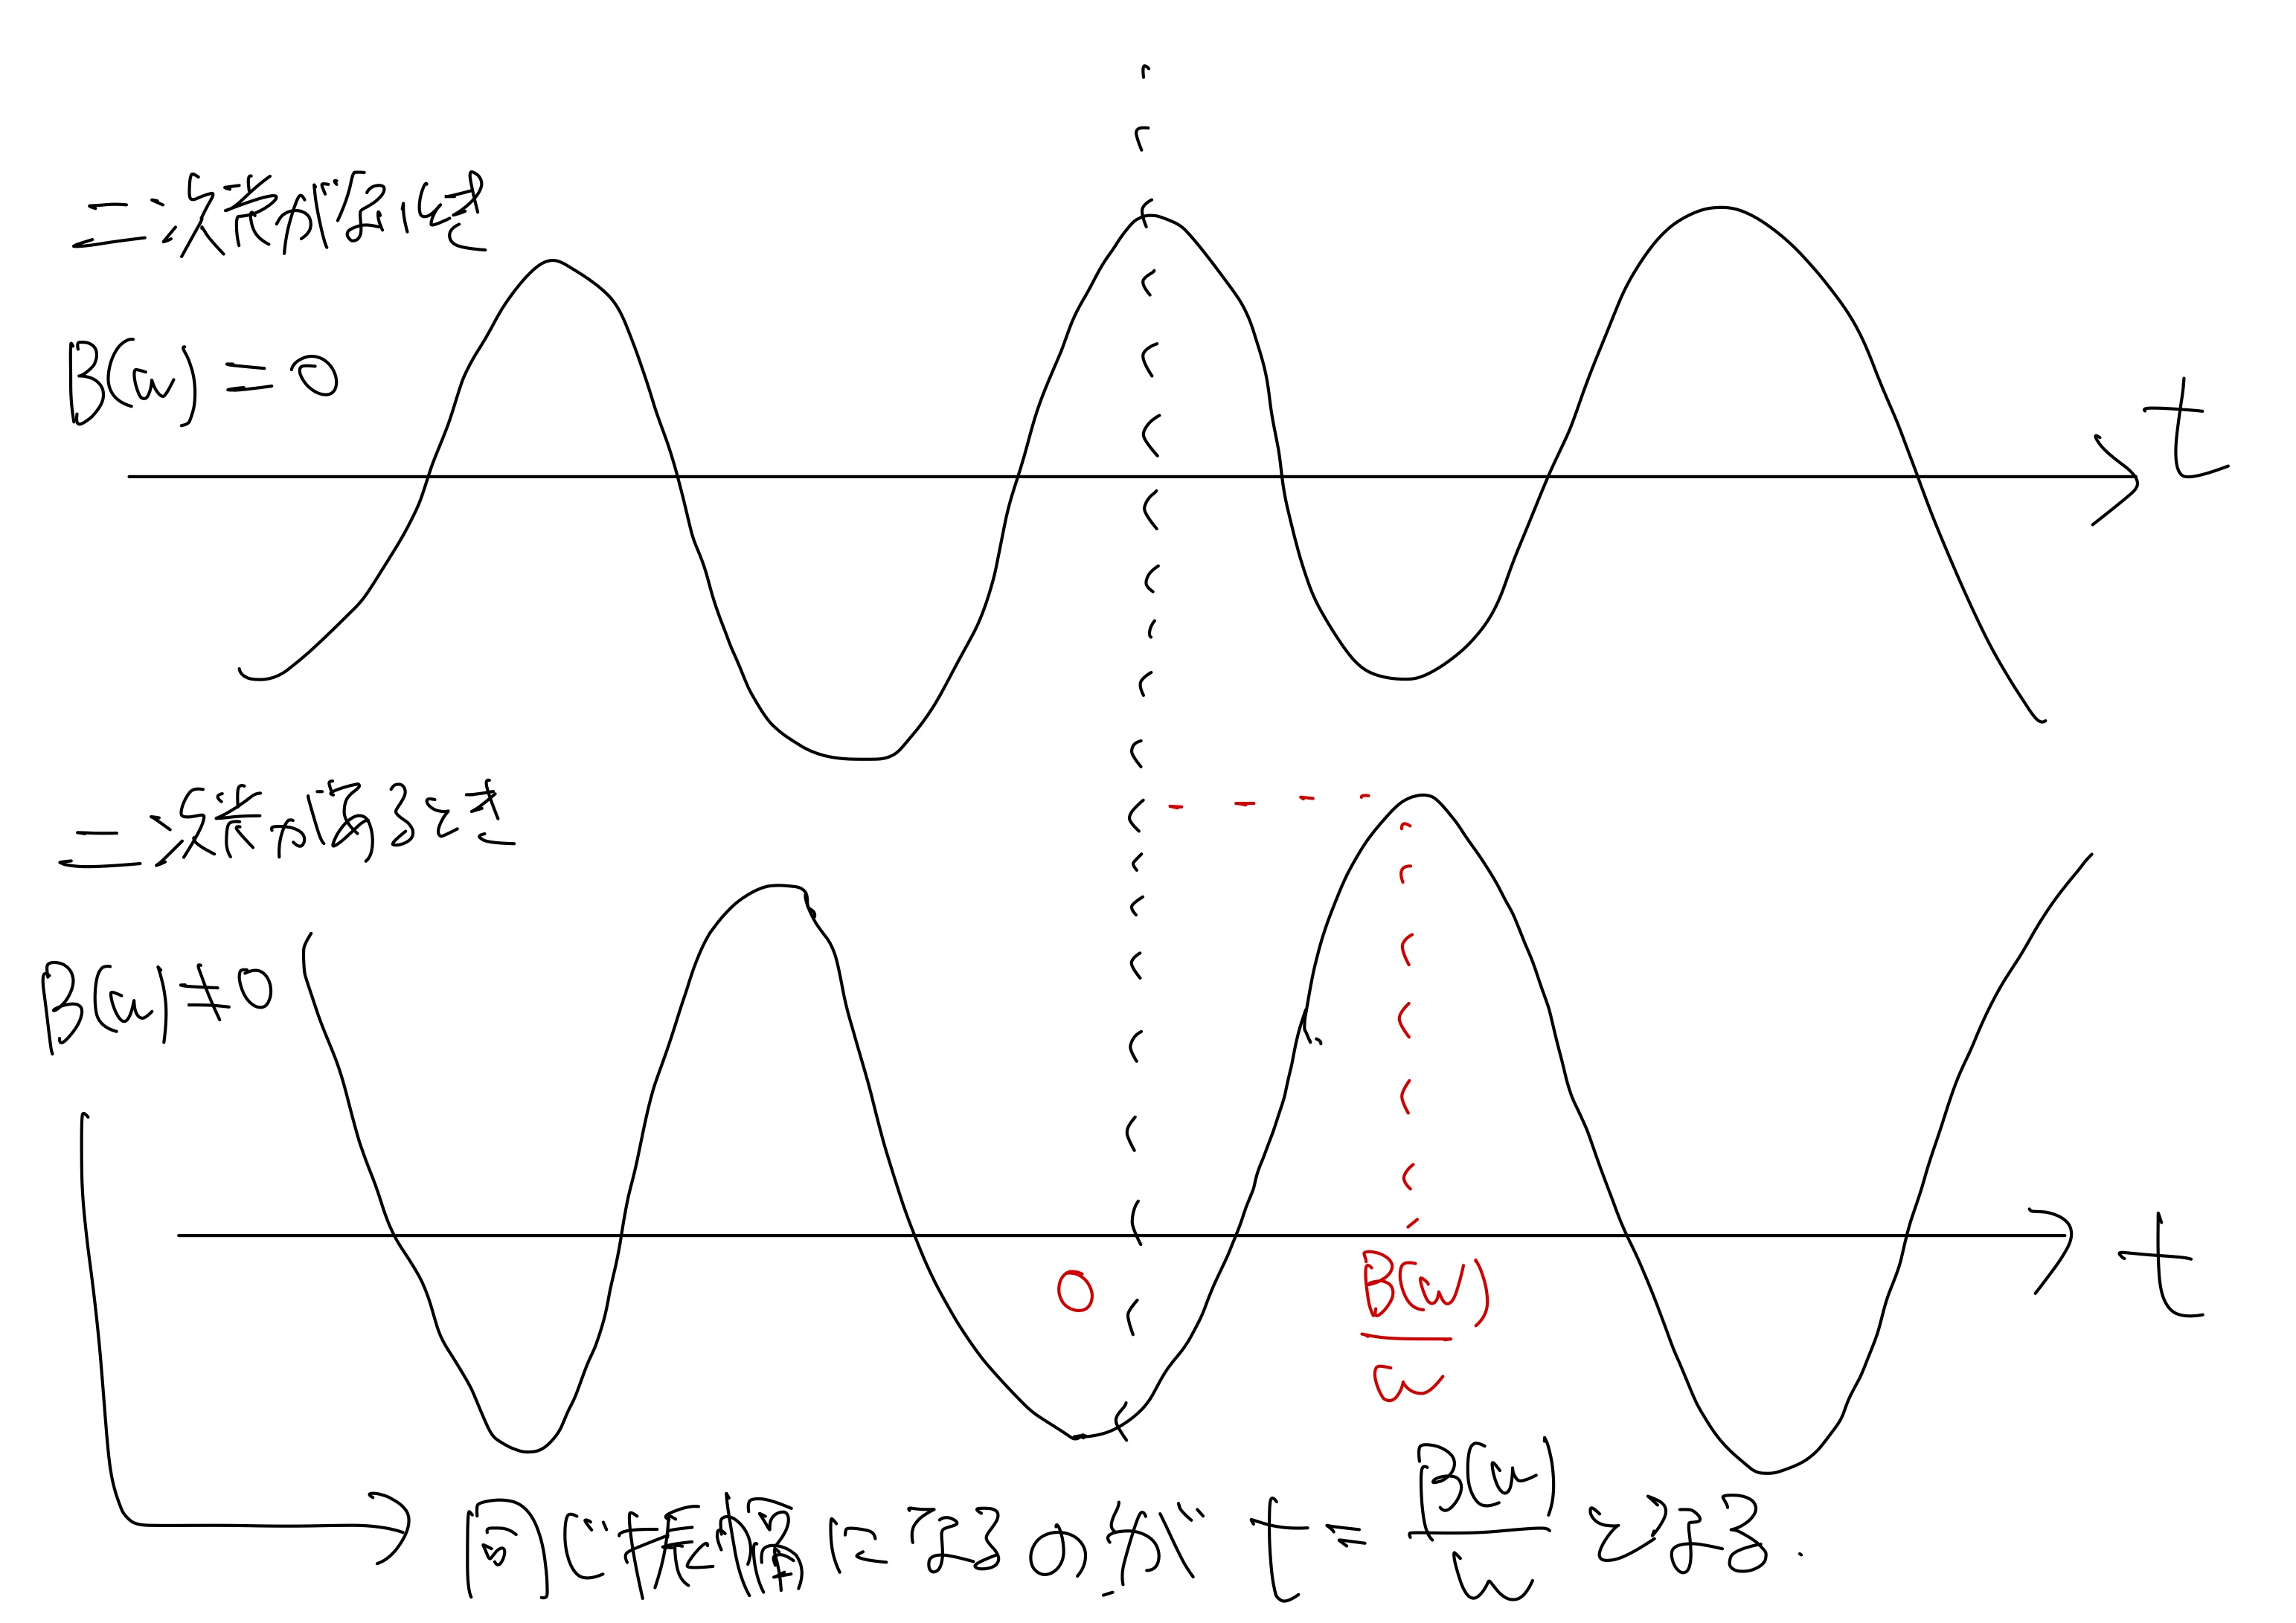
\includegraphics[width=0.5\textwidth]{fig2/Fig-7.jpg}
	%\caption{}
	\label{fig:fig2-Fig-7-jpg}
\end{figure}
\begin{tcolorbox}[colback=green!10!white]
	$B(\omega)>0$ ならば光は見かけ上遅れて見える。
\end{tcolorbox}
この見かけ上遅れる効果を屈折率で表す。

$B(\omega)=0$ のとき光は$\Delta z$ 進むのに$\Delta t=\Delta z /c$の時間がかかる。
一方で$B(\omega)\neq 0$ のときは$\Delta t= \frac{n}{c}\Delta z$ の時間がかかるとして$n$ を定義する。
その時間差は
\[
\frac{\Delta z}{c}(n-1)\to \frac{B(\omega)}{\omega}
.\] 
すなわち\eqref{eq:2-4}をもちいて変形していくと
\[
\frac{\Delta z}{c}(n-1)=\frac{B(\omega)}{\omega}=\frac{1}{E_0} \frac{eA(\omega)}{2\varepsilon_0 c}\times \eta=\frac{e^2}{2\varepsilon_0c}\frac{\eta}{m(\omega^2_0-\omega^2)}
.\] 
$N$ を単位体積当たりの原子数とすると
\[
\eta=N\times \Delta z
.\] 
したがって
\begin{equation}
\label{eq:2-12}
	n=1+\frac{Ne^2}{2\varepsilon_0m}\frac{1}{\omega_0^2-\omega^2}
.\end{equation}
第二項が2次光の効果である。
\begin{figure}[H]
	\centering
	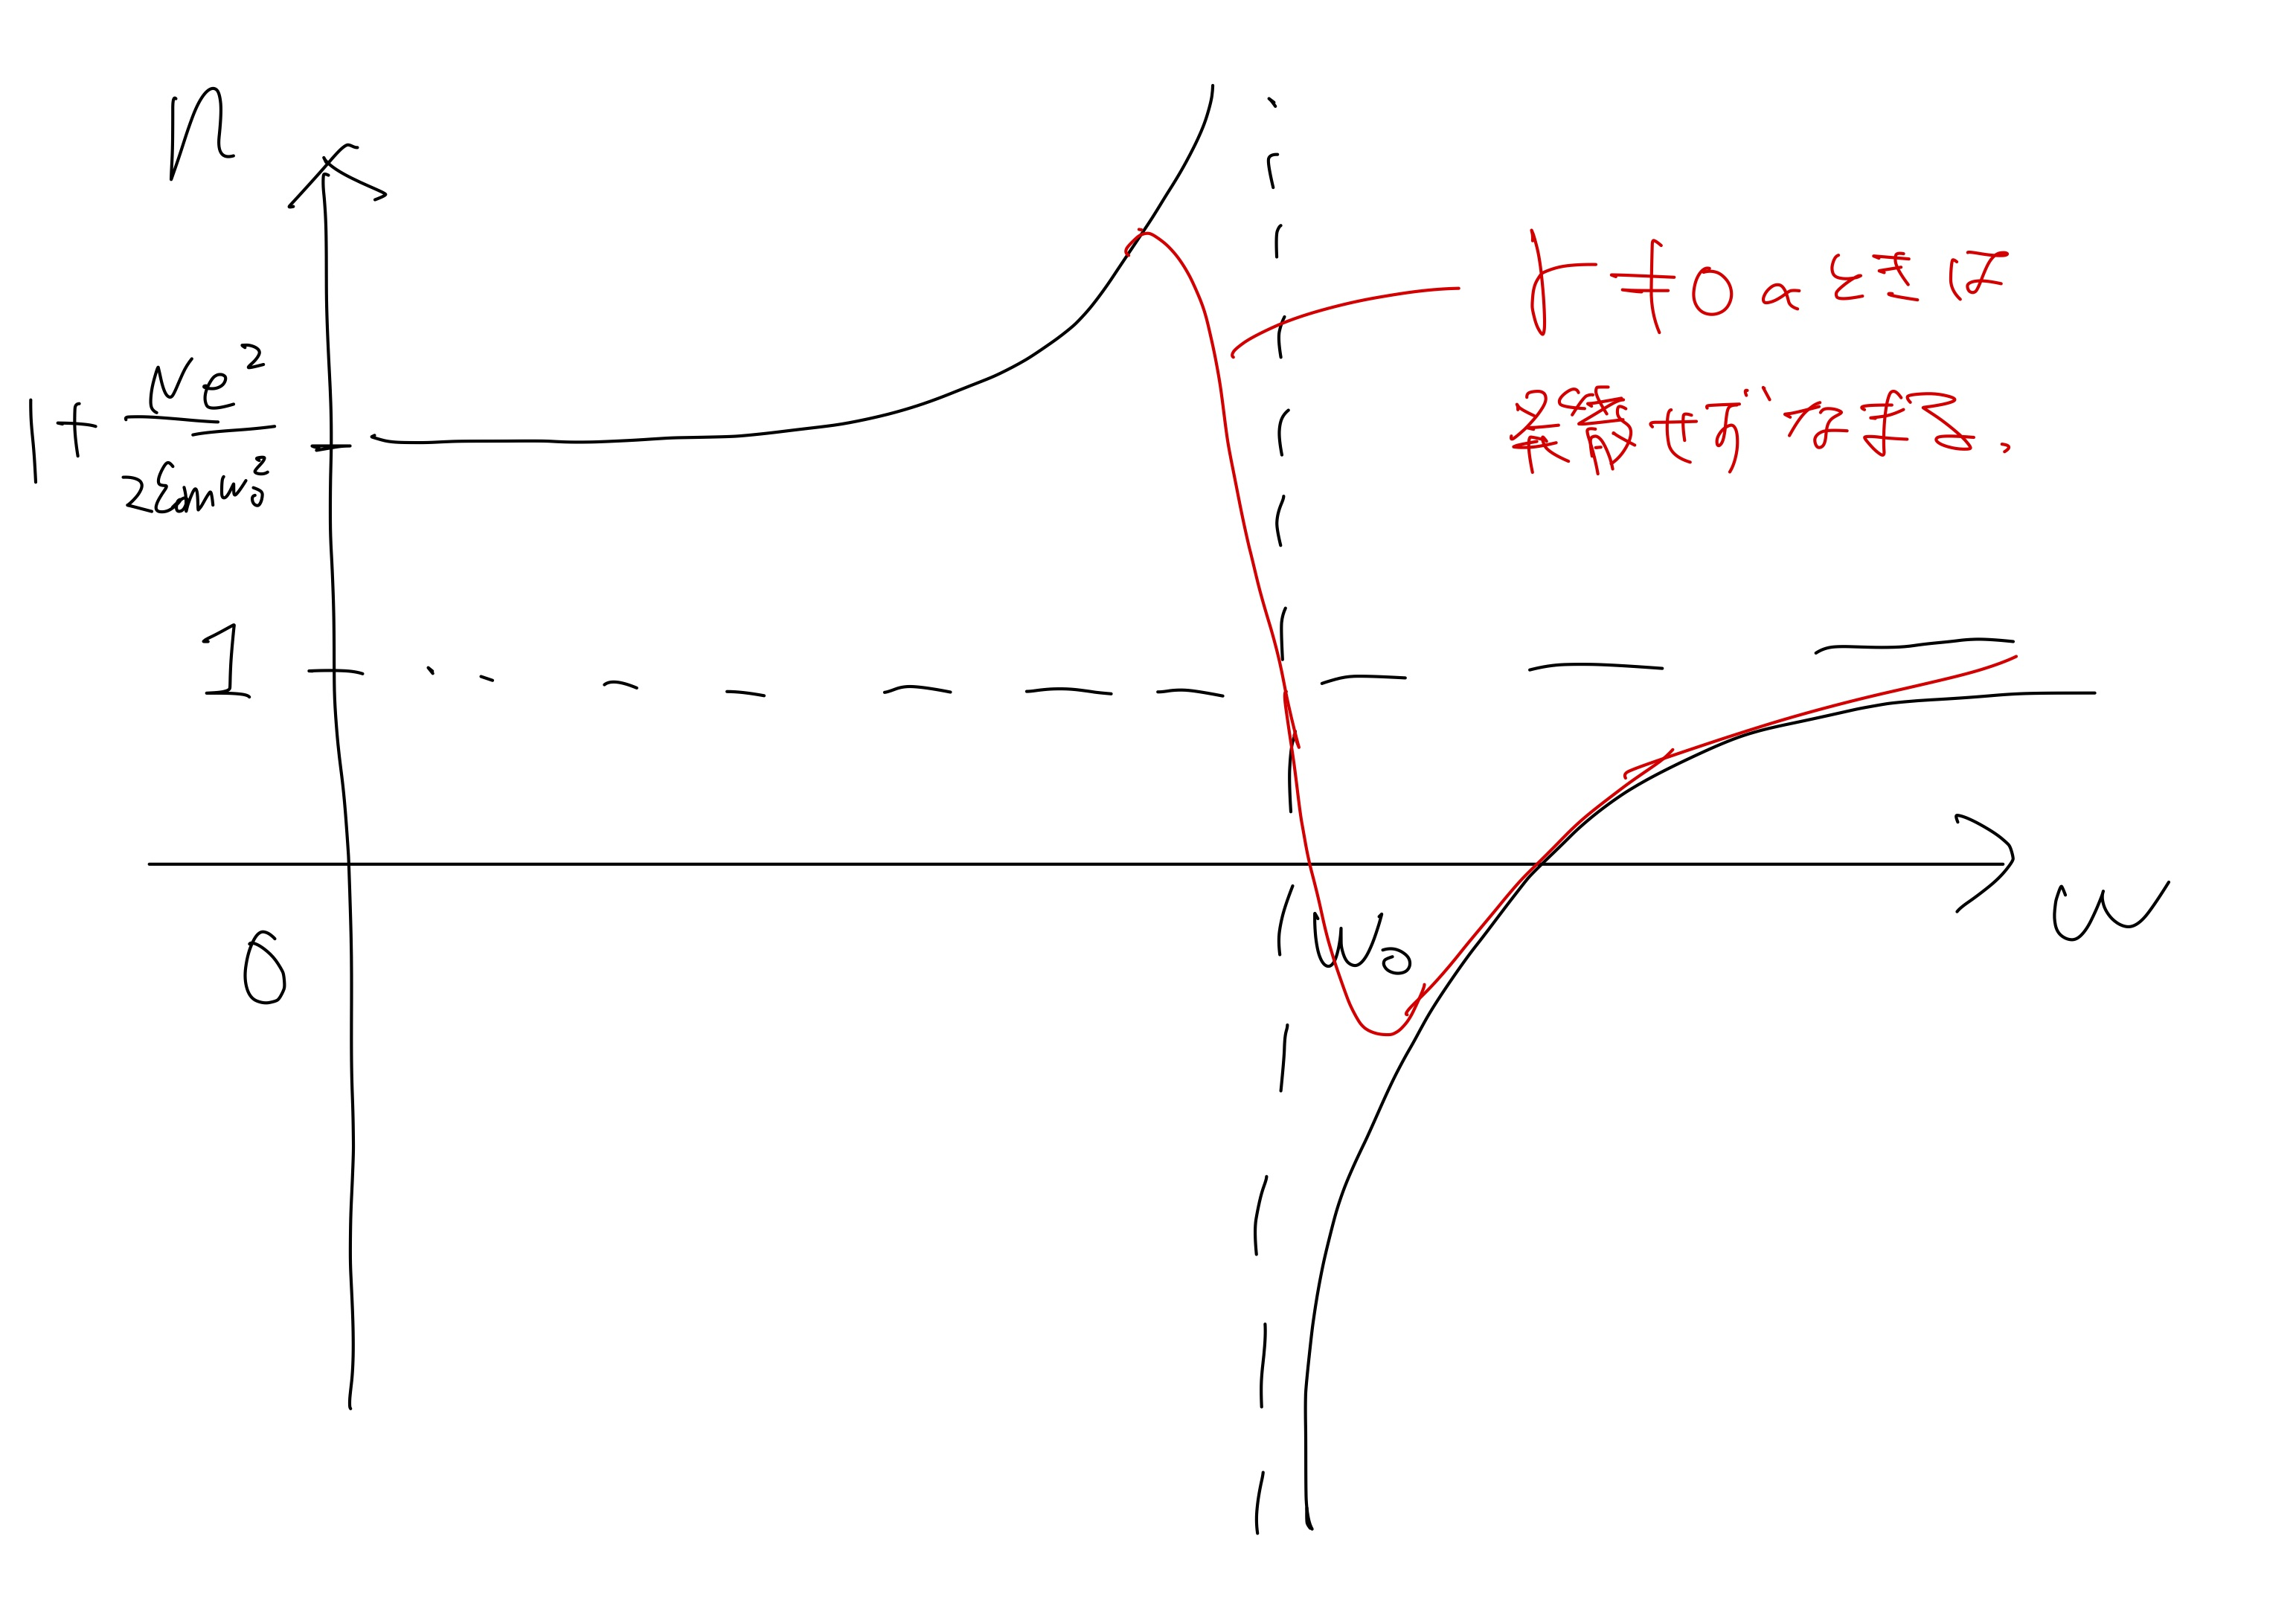
\includegraphics[width=0.5\textwidth]{fig2/Fig-8.jpg}
	%\caption{}
	\label{fig:fig2-Fig-8-jpg}
\end{figure}
$\omega>\omega_0$ のとき$n<1$ となってこのとき$B(\omega)<0$ だから\eqref{eq:2-11}
光は見かけ上真空より早く進む。
光の\textcolor{red}{位相速度}は光速を超えることがある。

2022/10/20/num3

\subsection{物質中の光の波長の意味}
このsubsectionでは江馬先生の光物理学の基礎という本を用いている。


原子シートモデルというのを考えた。
これは物質を原子シートが何枚も重なったものと考える。
\begin{figure}[H]
	\centering
	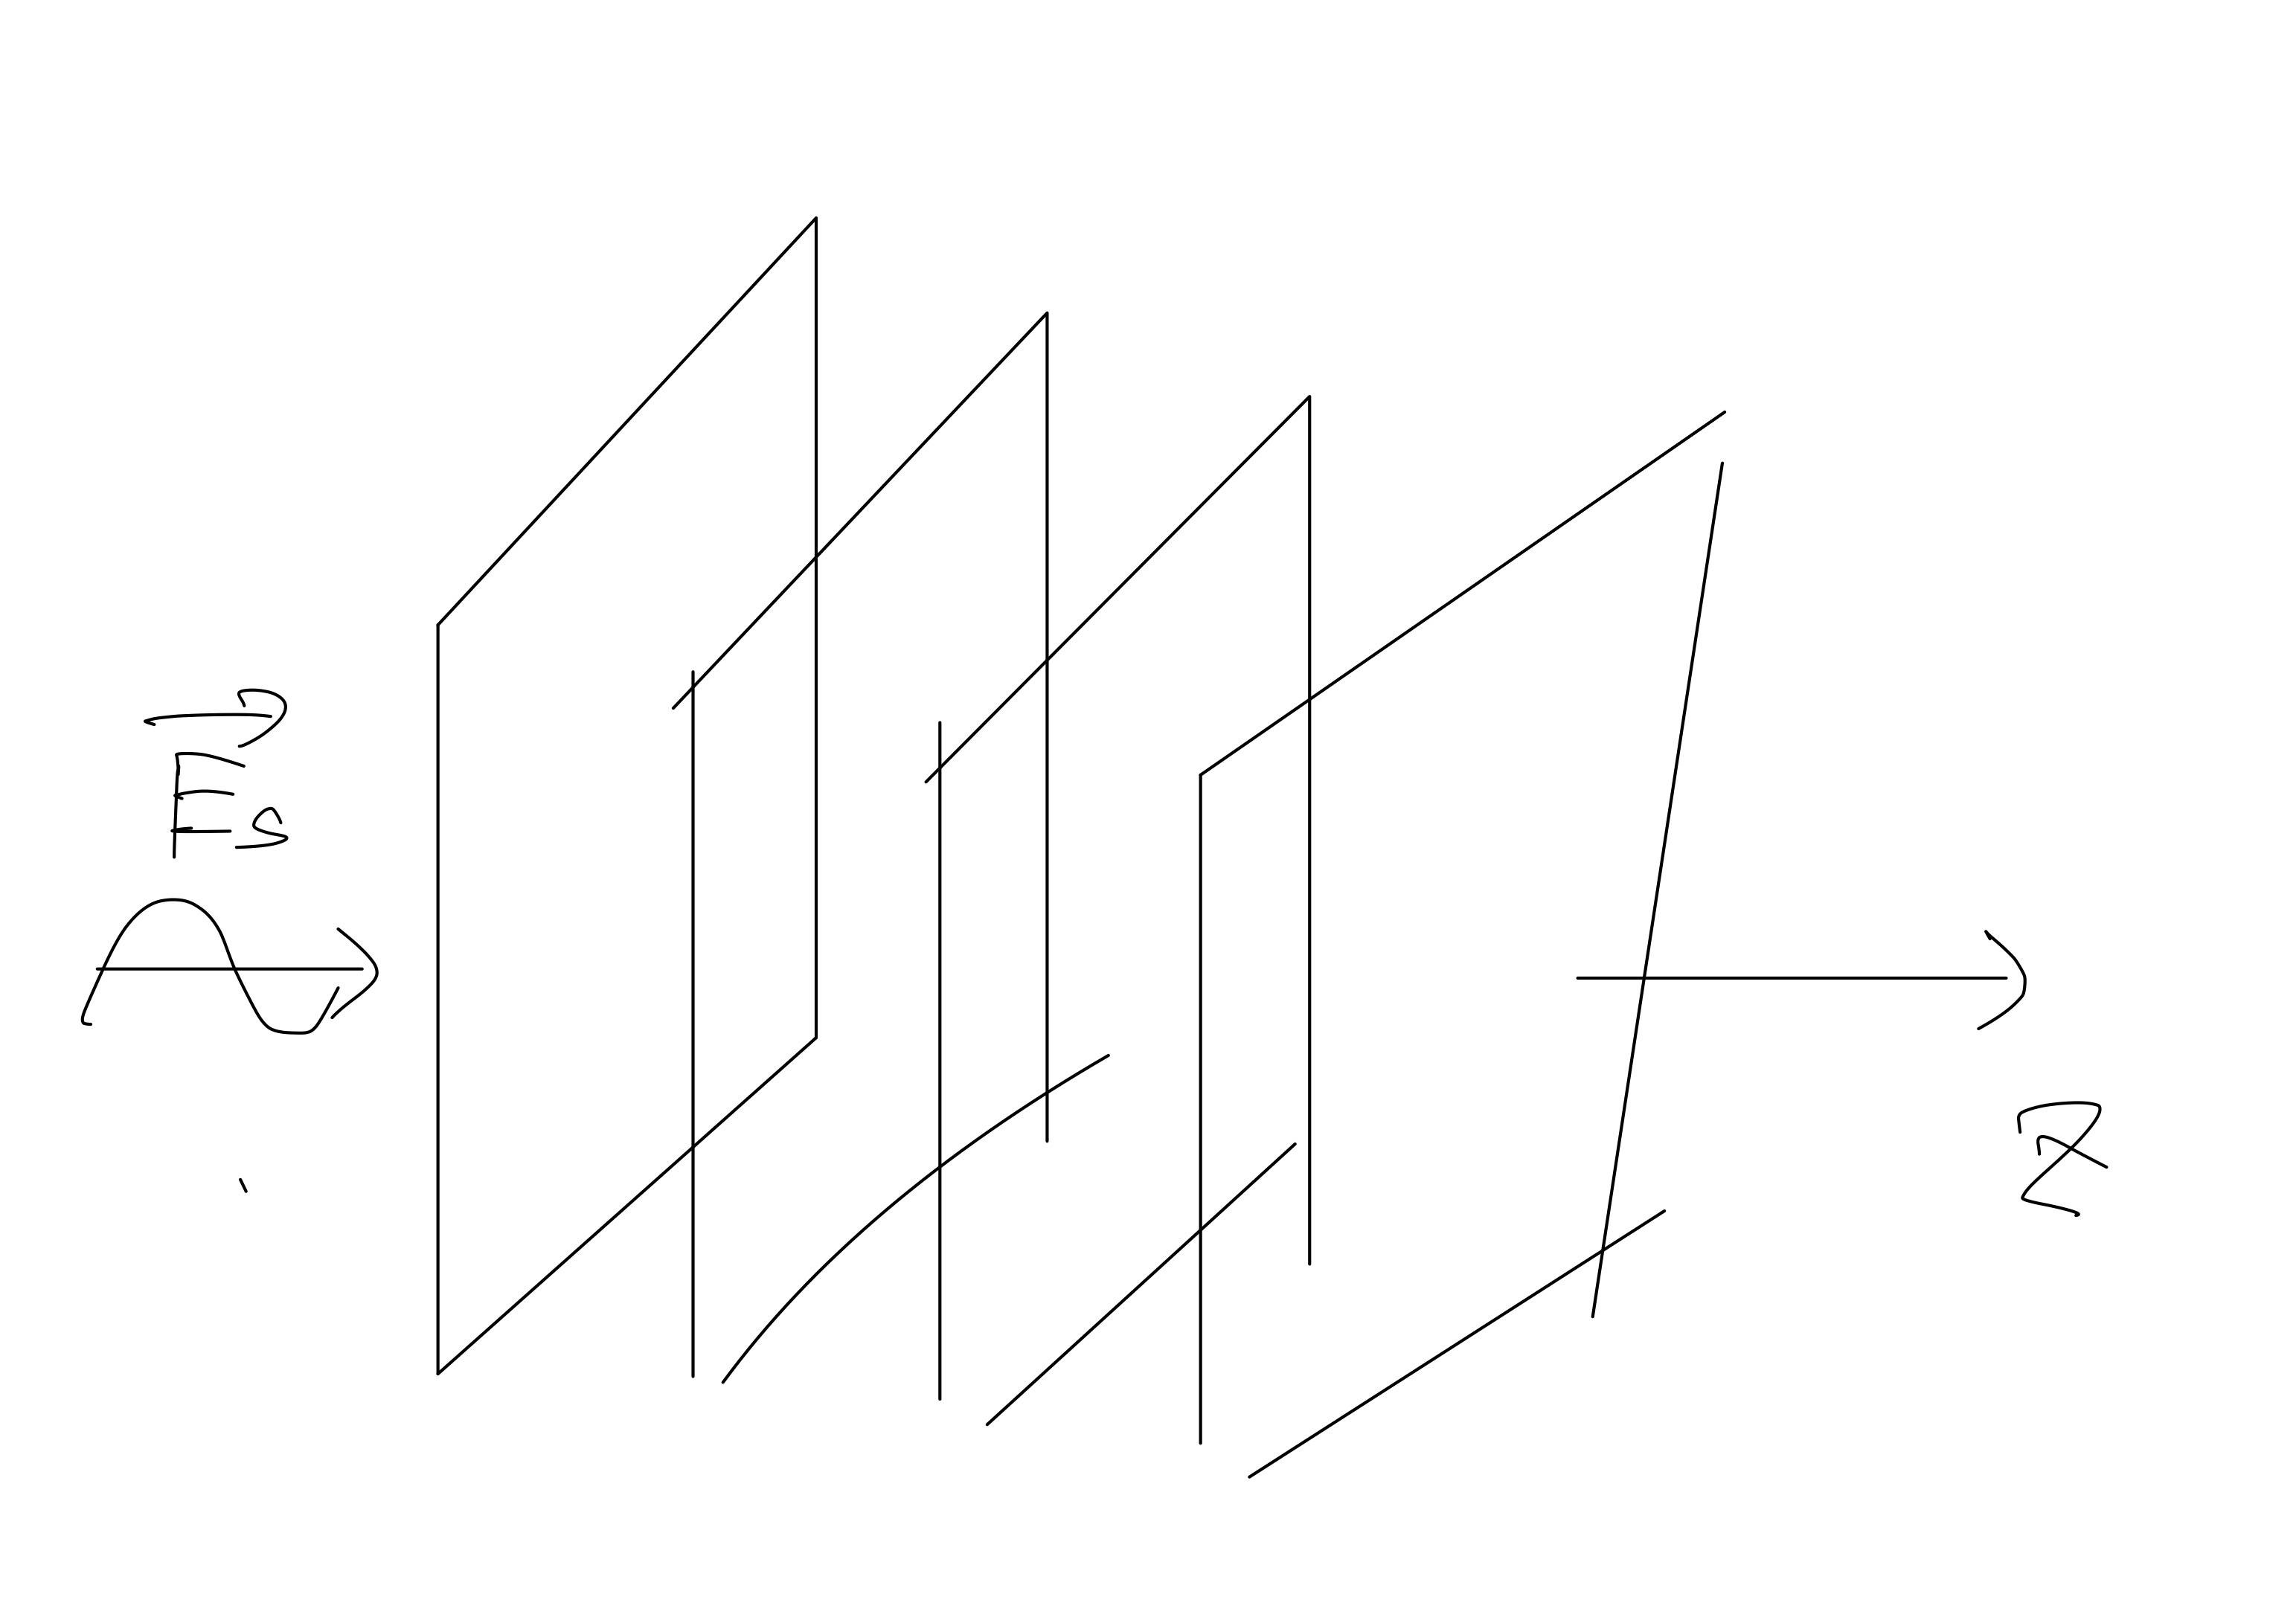
\includegraphics[width=0.5\textwidth]{fig3/Fig-2.jpg}
	%\caption{fig3/Fig-2.jpg}
	\label{fig:fig3-Fig-2-jpg}
\end{figure}

\begin{figure}[H]
	\centering
	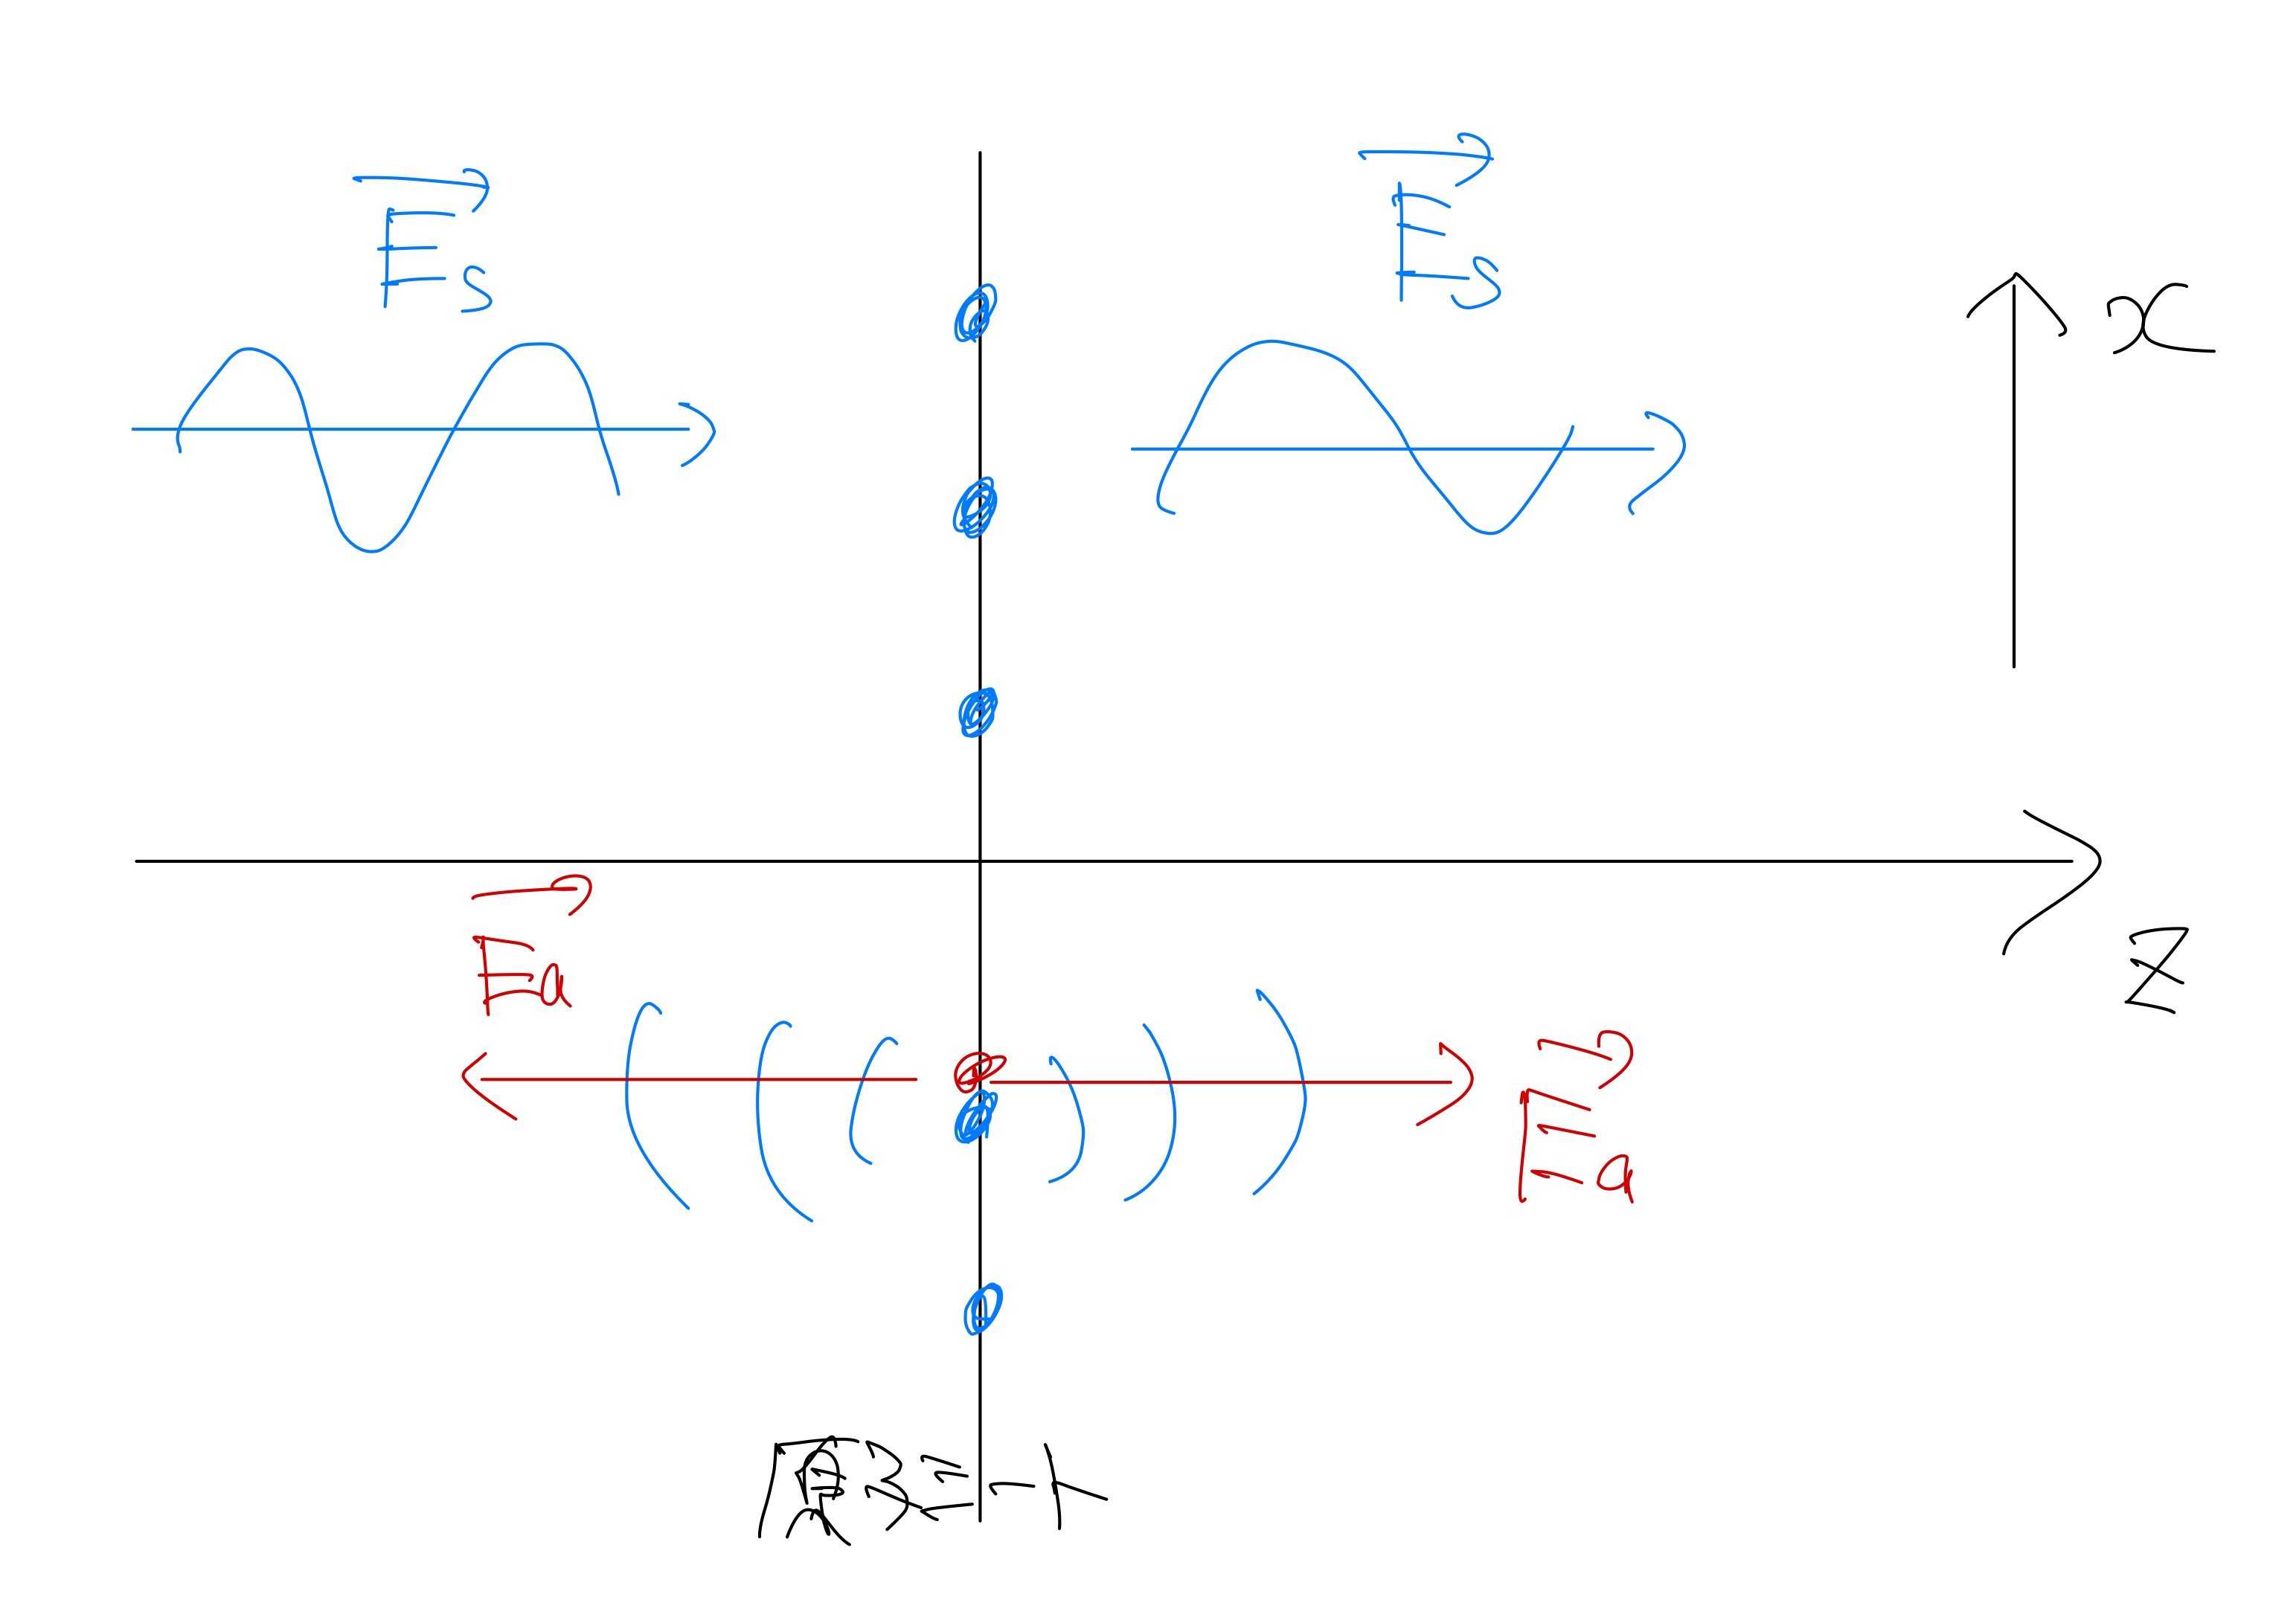
\includegraphics[width=0.5\textwidth]{fig3/Fig-3.jpg}
	%\caption{fig3/Fig-3.jpg}
	\label{fig:fig3-Fig-3-jpg}
\end{figure}

\[
E_s=E_0e^{i(kz-\omega t)}
.\] 
\[
	E_a=\tilde{r}E_s=\tilde{r}E_0e^{i(kz-\omega t)}
.\] 
\begin{equation}
\label{eq:3-13}
E_r=\tilde{r}E_0e^{-i(kz+\omega t)}
.\end{equation}
ただし位相のズレがあるため$\tilde{r}$ は複素数である
\begin{equation}
\label{eq:3-14}
\tilde{r}=re^{i\delta}
.\end{equation}
透過光を$E_1$とおくと
\begin{equation}
\label{eq:3-15}
	E_1=E_s+E_a=E_0(1+re^{i\delta})e^{i(kz-\omega t)}
.\end{equation}
ここで$(1+re^{i\delta})$ の項では\textcolor{red}{エネルギーは増えないから$E_s$ と$E_a$は干渉で弱め合うはずである。}
位相のズレを調べる。
エネルギー保存則から
\begin{equation}
\label{eq:3-16}
	\abs{E_s}^2=\abs{E_1}^2+\abs{E_r}^2
.\end{equation}
でなければならない。
	\[
	E_0^2=E_0^2(1+r^2+2r\cos \delta+r^2)
	.\] 
	ゆえに
	\begin{equation}
	\label{eq:3-17}
		\cos \delta=-r
	.\end{equation}
	\eqref{eq:3-15}から
\begin{equation}
\label{eq:3-18}
	\abs{E_1}=E_0\sqrt{1-r^2} 
.\end{equation}
\[
\abs{1+re^{i\delta}}=\sqrt{1+r^2+2r\cos \delta} =\sqrt{1-r^2} 
.\] 
この辺は位相が変わってたされたので振幅が減ってエネルギー的にはあっているということになる。

\eqref{eq:3-15}の$E_1$ を
\begin{equation}
\label{eq:3-19}
E_1=\abs{E_1}e^{i\delta_1}e^{i(kz-\omega t)}
.\end{equation}
とかくと
\[
\sin \delta_1=r
.\] 
となる。いまからこれを導く。
\eqref{eq:3-15}と\eqref{eq:3-19}より
\[
E_0(1+re^{i\delta})=\abs{E_{1}}e^{i\delta_1}
.\] 
虚部を比較して
\begin{equation}
\label{eq:3-19'}
E_0 r\sin \delta=\abs{E_1}\sin \delta_1
.\end{equation}
ここで\eqref{eq:3-17}より
\[
\sin \delta=\sqrt{1-\cos ^2\delta} =\sqrt{1-r^2} 
.\] 
また\eqref{eq:3-18}より
\begin{equation}
\label{eq:3-19''}
	\abs{E_1}=E_0\sqrt{1-r^2} =E_0\sin \delta
.\end{equation}
\eqref{eq:3-19'}と\eqref{eq:3-19''}より
\begin{equation}
\label{eq:3-20}
	\sin \delta_1=r
.\end{equation}
\begin{figure}[H]
	\centering
	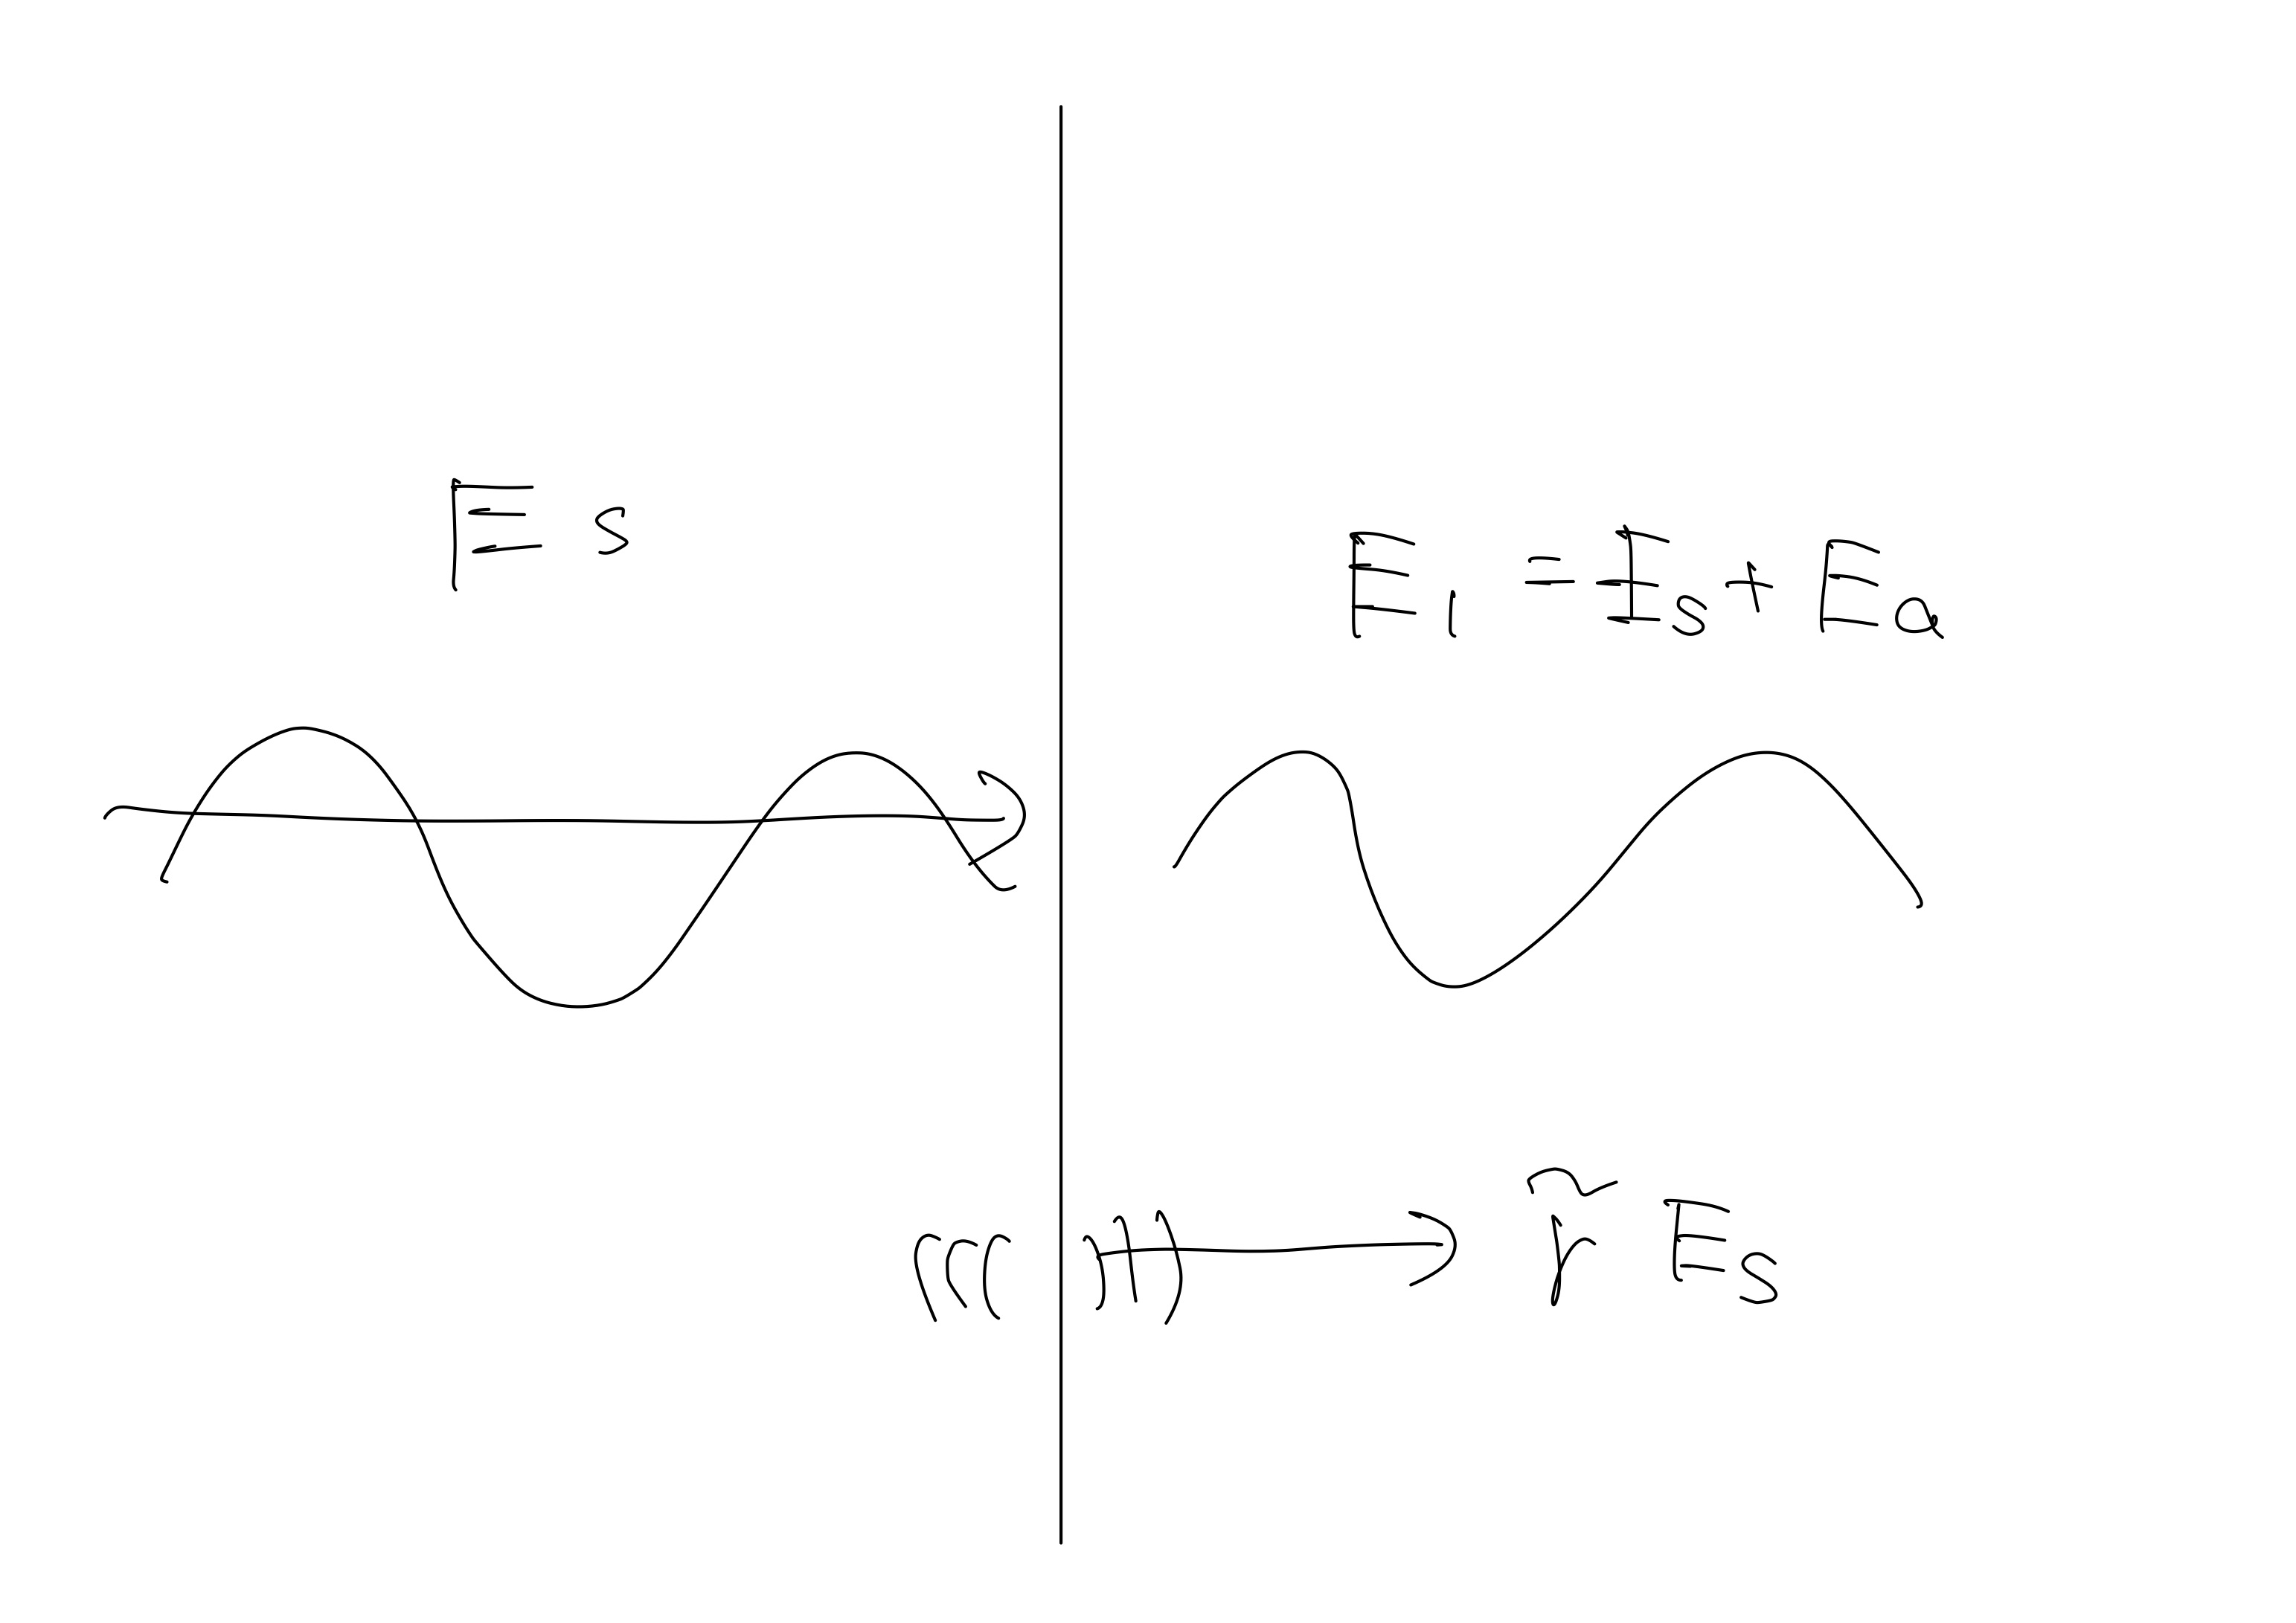
\includegraphics[width=0.5\textwidth]{fig3/Fig-4.jpg}
	%\caption{fig3/Fig-4.jpg}
	\label{fig:fig3-Fig-4-jpg}
\end{figure}

ここで$r\ll 1$ ならば
\begin{equation}
\label{eq:3-21}
	\delta_1\sim r
.\end{equation}
すなわち原子シート一枚で位相が$r$ ずれる。
なお\eqref{eq:2-10}より位相のずれ
は$B(\omega)=\omega /c A(\omega)$だから
\begin{equation}
\label{eq:3-22}
r \propto \frac{\omega}{c}A(\omega)
.\end{equation}
が成り立つ。
\begin{figure}[H]
	\centering
	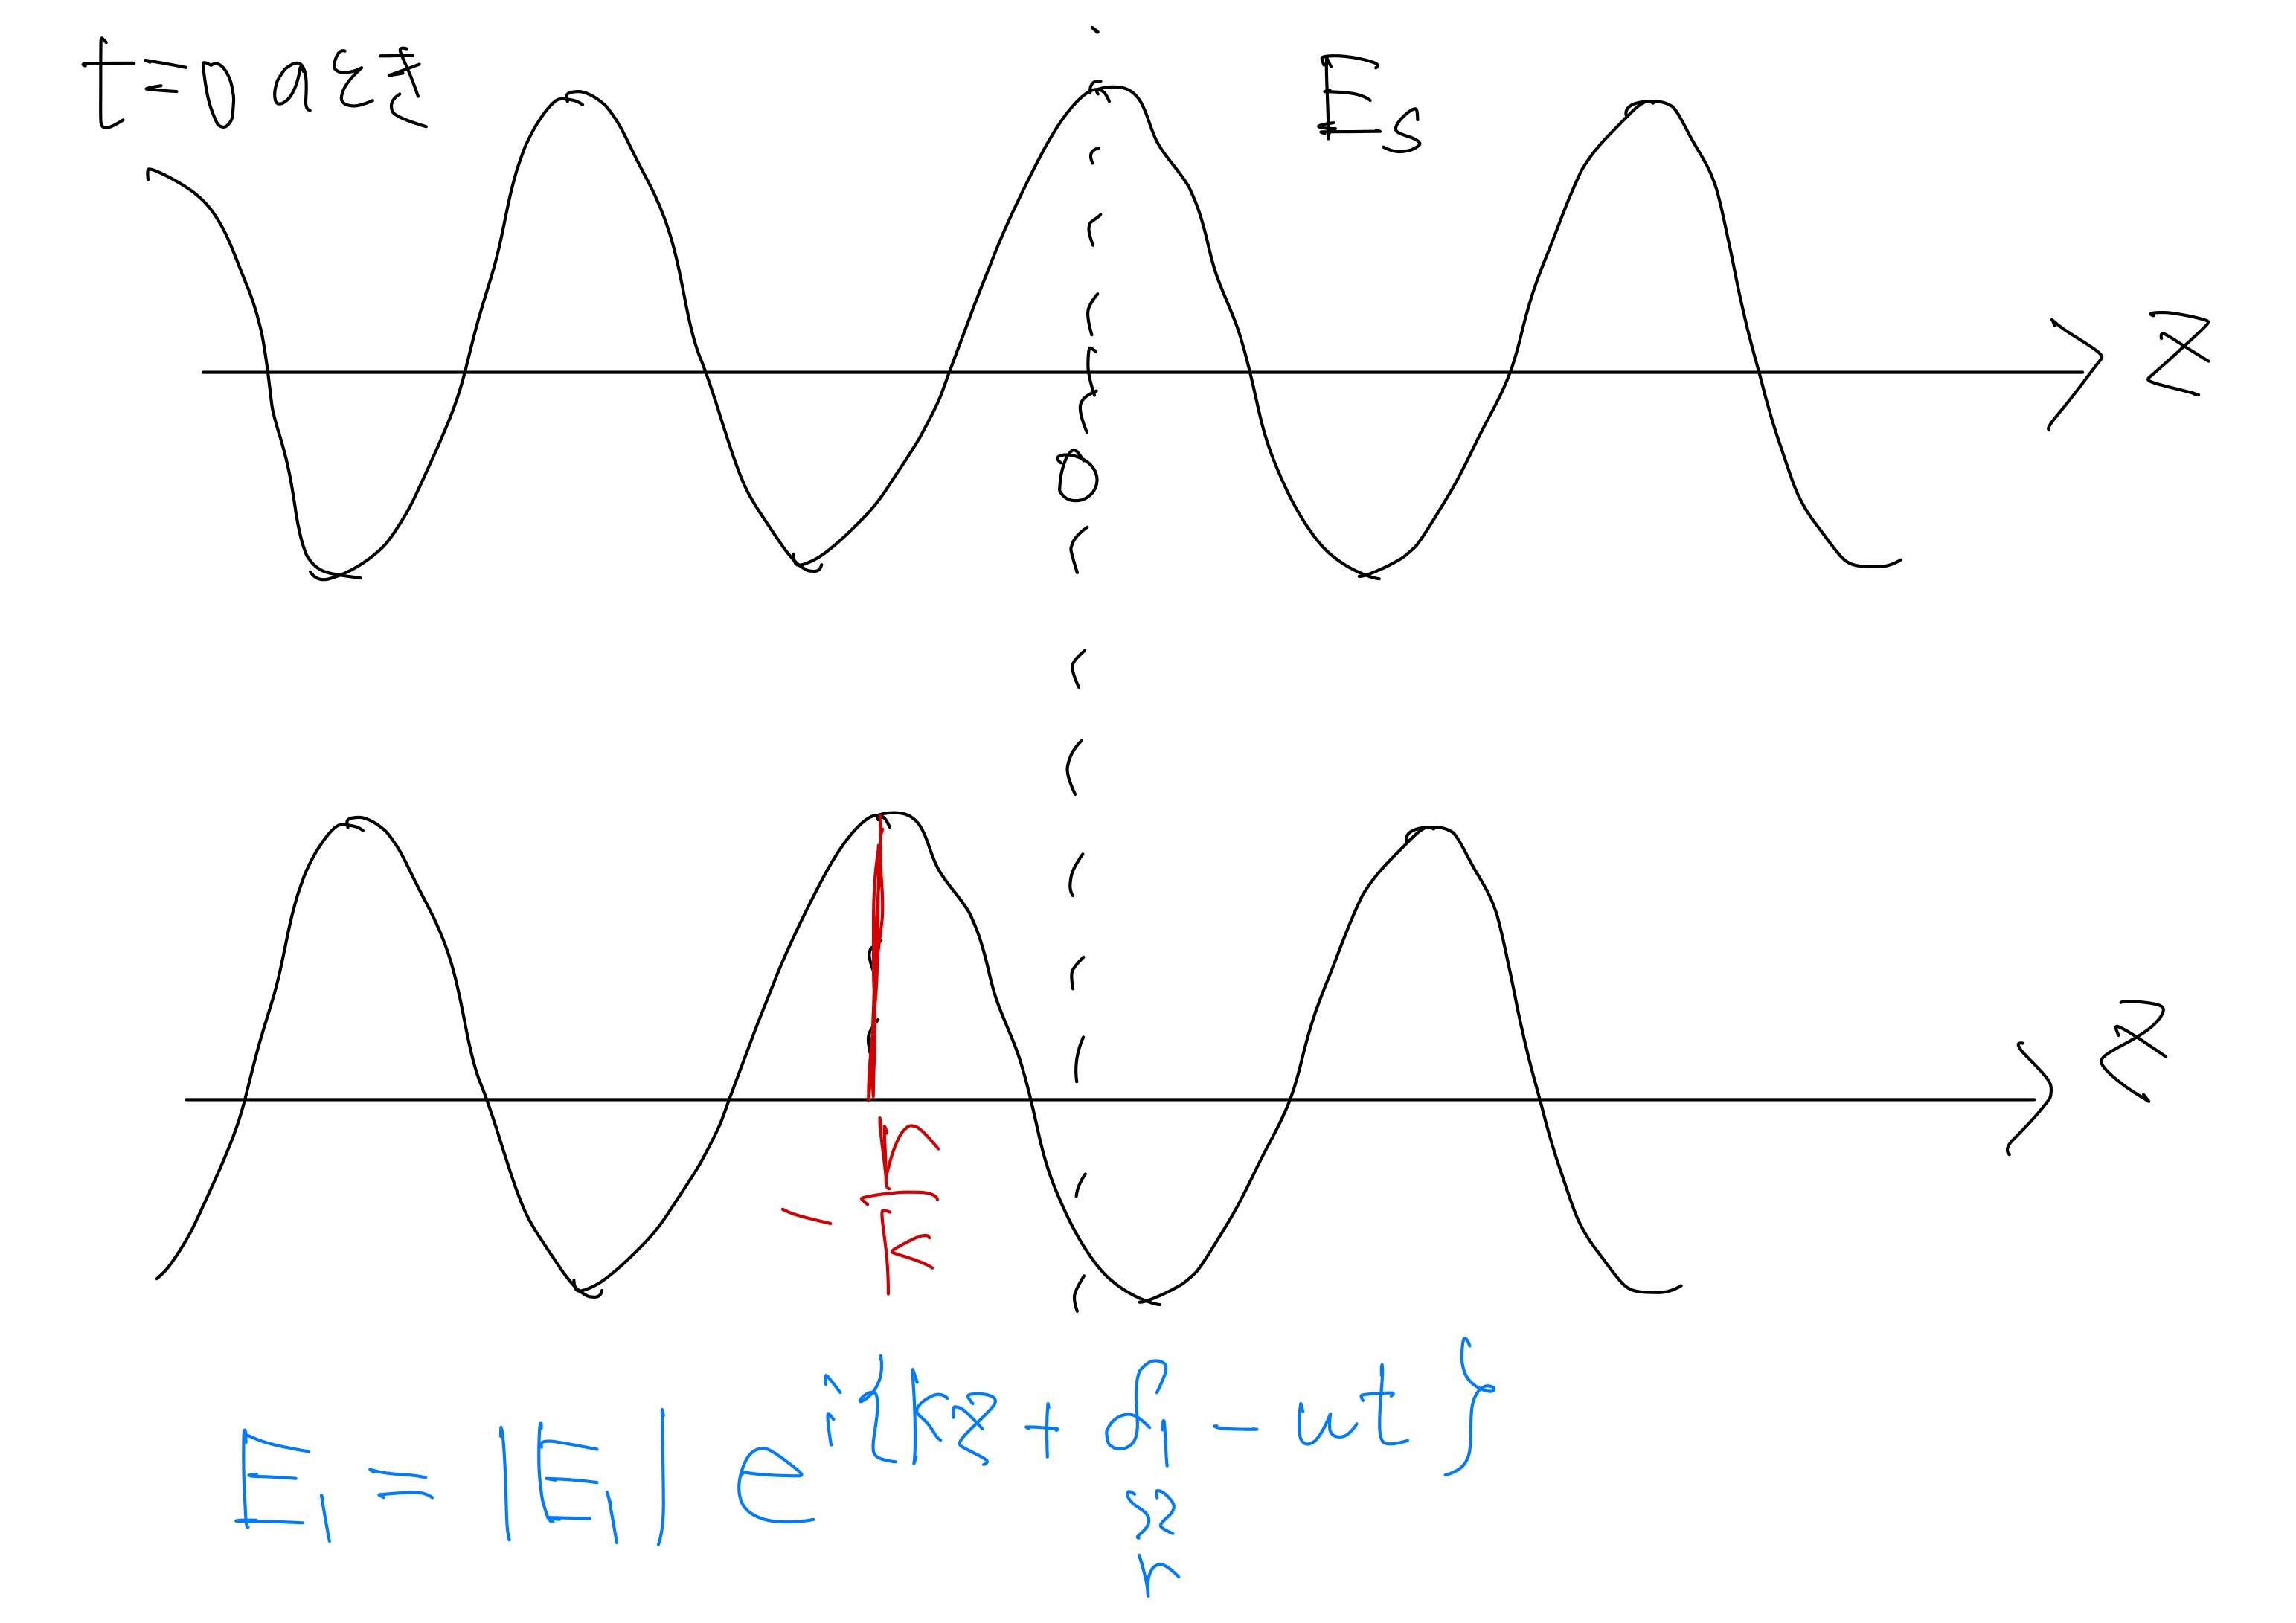
\includegraphics[width=0.5\textwidth]{fig3/Fig-5.jpg}
	\caption{fig3/Fig-5.jpg}
	\label{fig:fig3-Fig-5-jpg}
\end{figure}
原子一層通過すると正弦波が$-r /k$ だけずれる。
\begin{figure}[H]
	\centering
	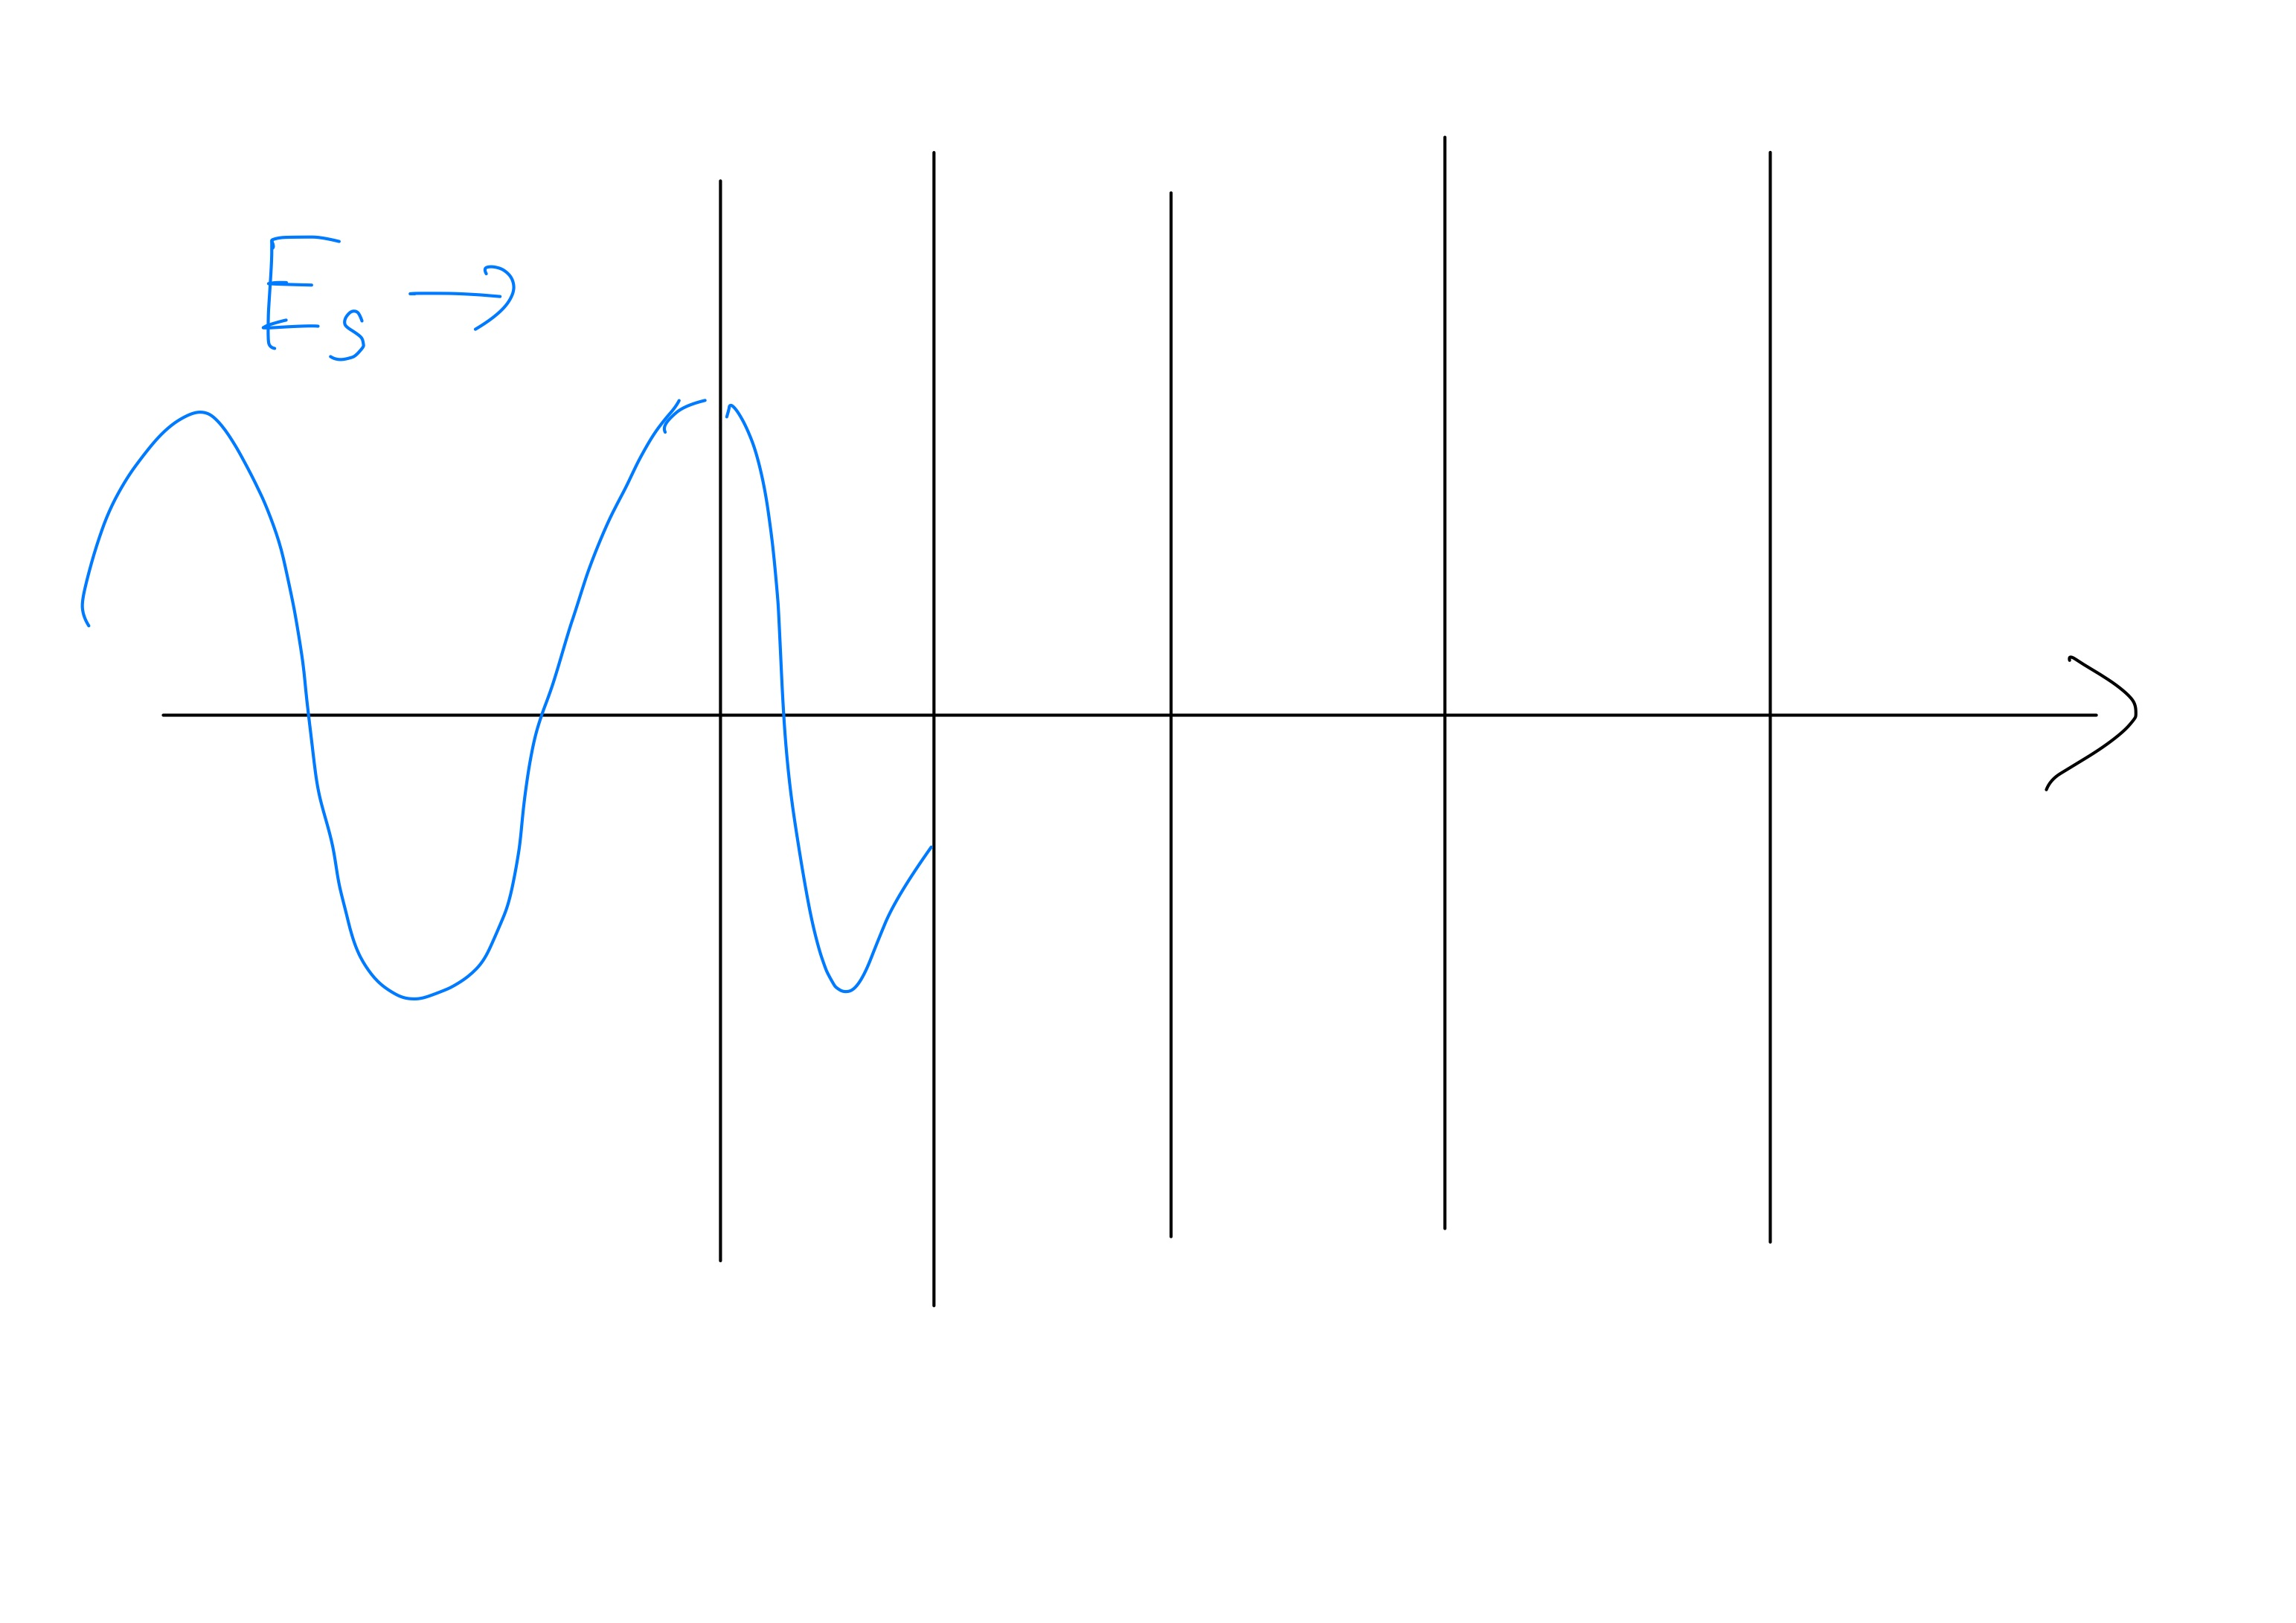
\includegraphics[width=0.5\textwidth]{fig3/Fig-6.jpg}
	\caption{fig3/Fig-6.jpg}
	\label{fig:fig3-Fig-6-jpg}
\end{figure}
$m$ 層通過すると$-r /k \cdot m$だけずれる。
原子層の幅を$l$ として
\begin{figure}[H]
	\centering
	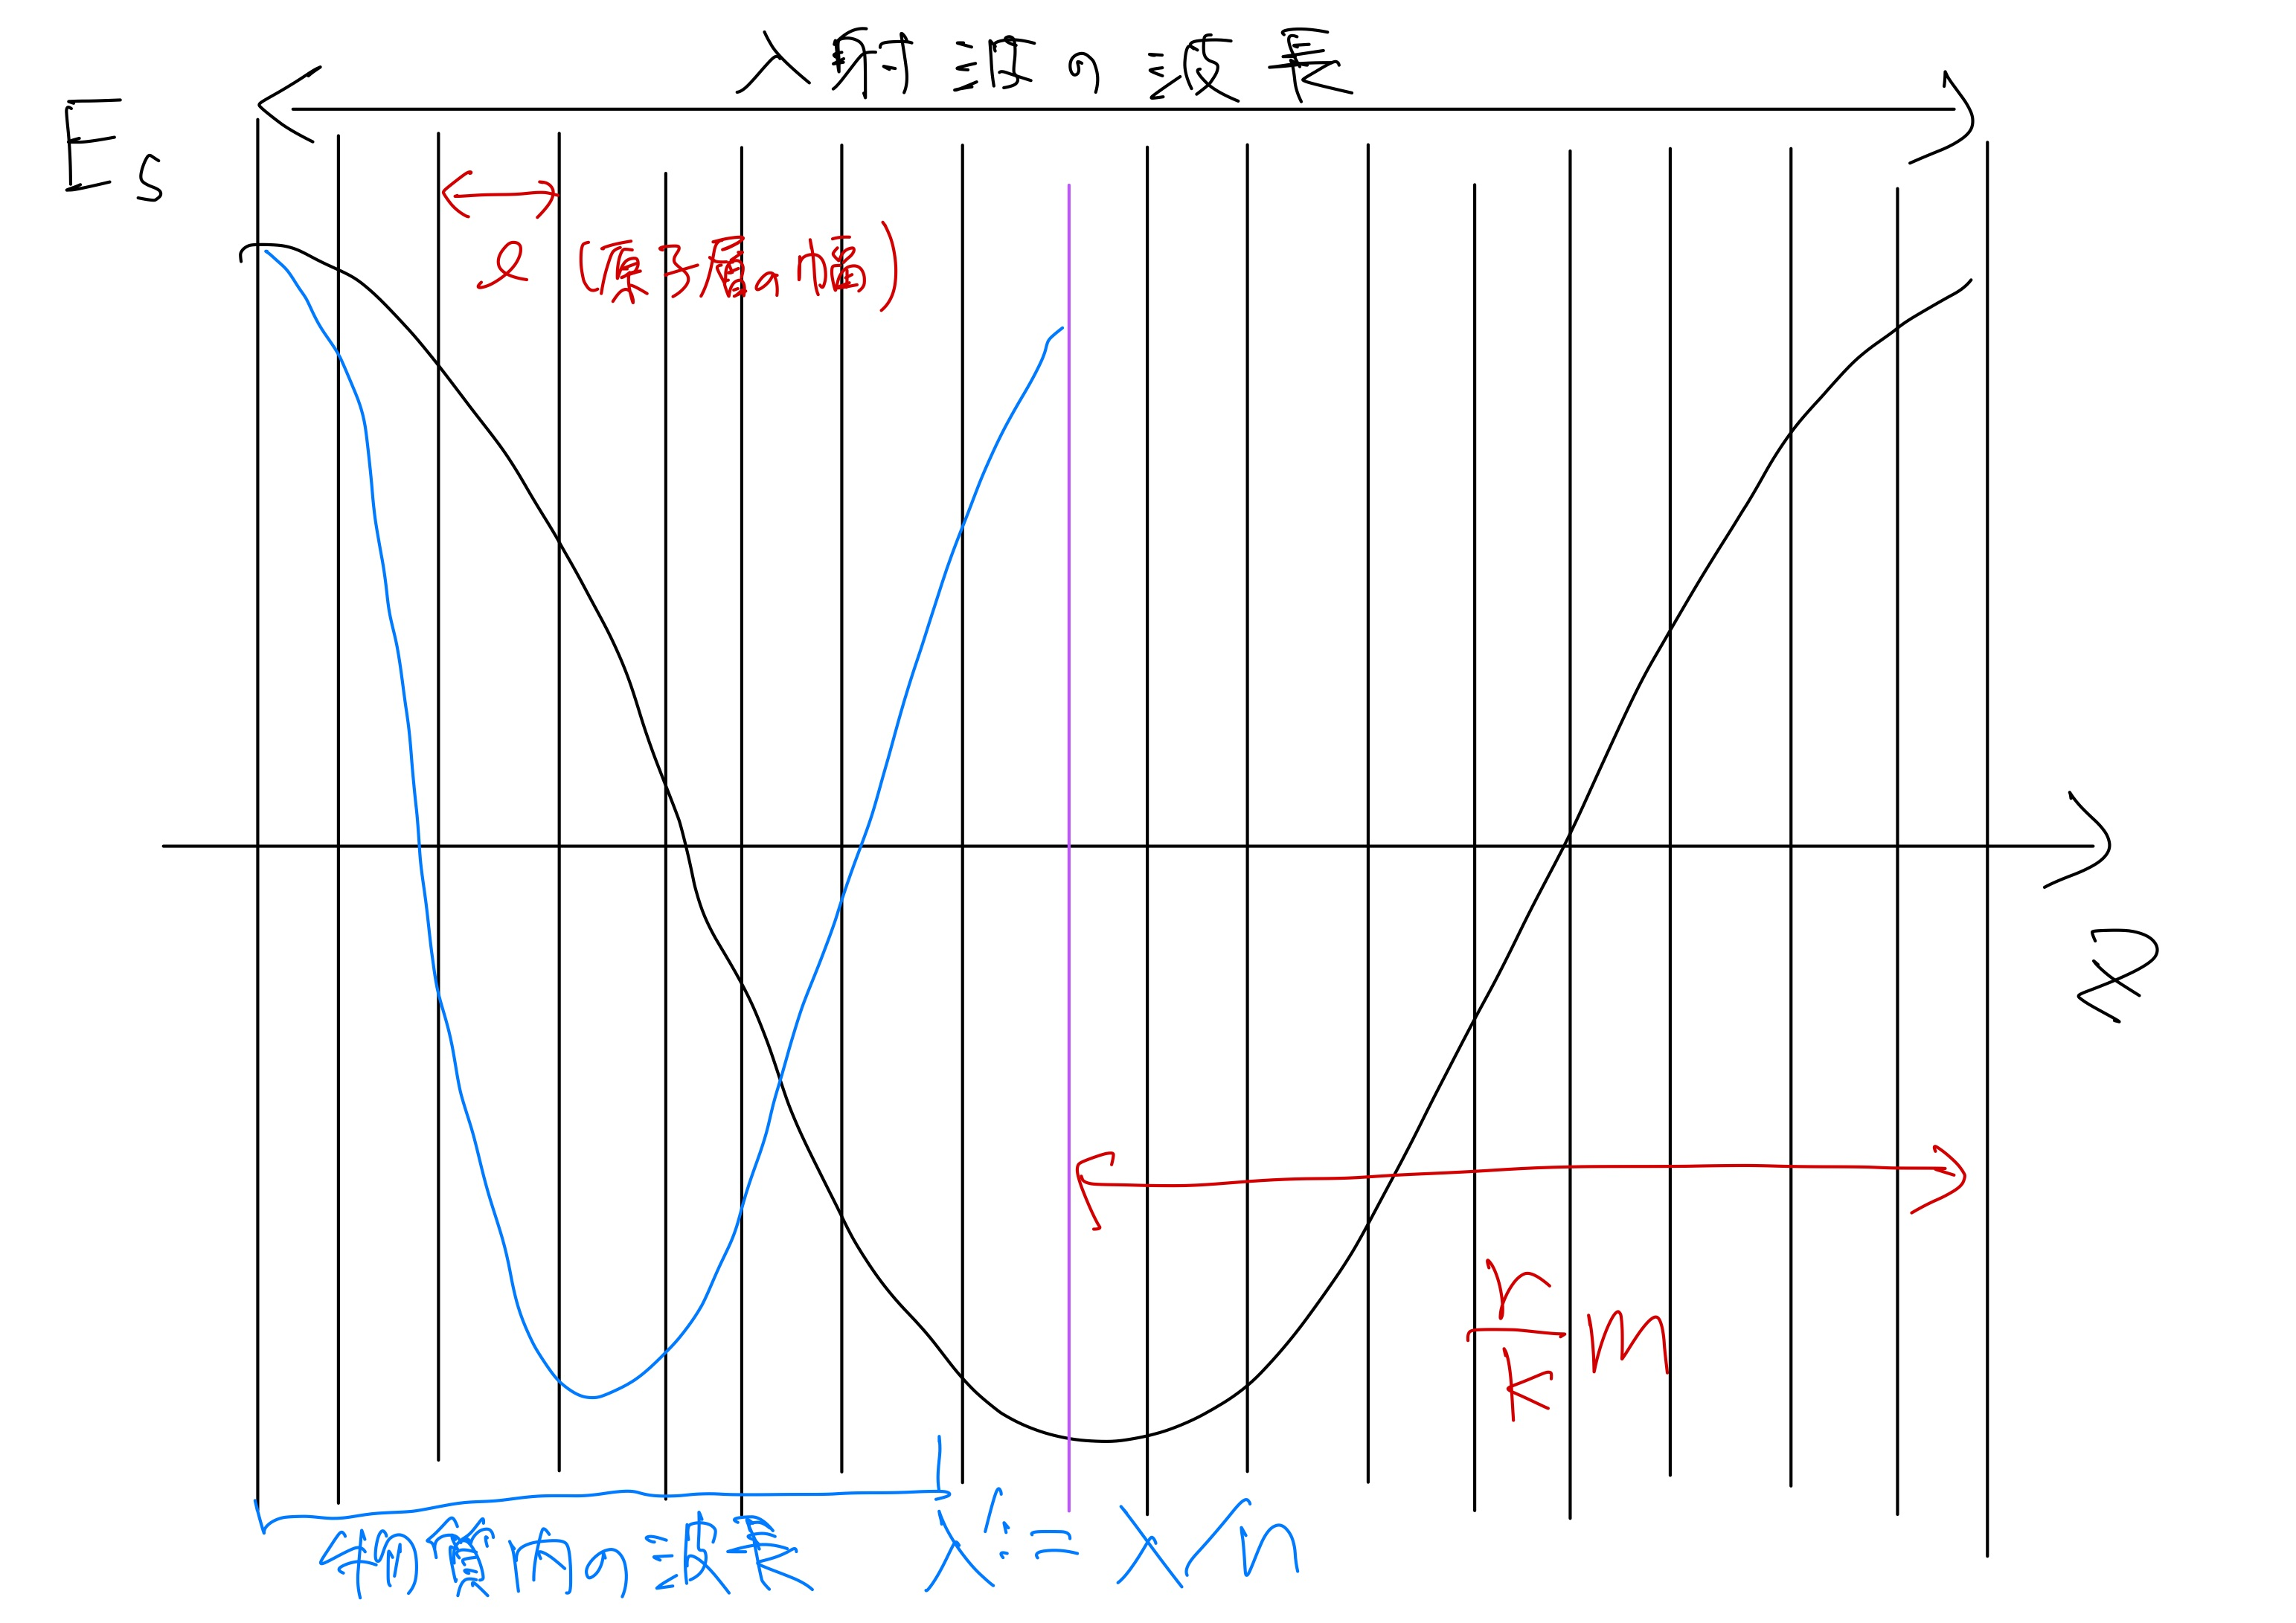
\includegraphics[width=0.5\textwidth]{fig3/Fig-7.jpg}
	\caption{fig3/Fig-7.jpg}
	\label{fig:fig3-Fig-7-jpg}
\end{figure}
したがって図より
\begin{equation}
\label{eq:3-23}
	\lambda'=\lambda-\frac{r}{k}m
.\end{equation}
$m$ は$\lambda'$ の間に通過したシート数なので
\begin{equation}
\label{eq:3-24}
	m=\frac{\lambda'}{l}
.\end{equation}
\eqref{eq:3-23}と\eqref{eq:3-24}と$\lambda' = \lambda /n$ から
\begin{equation}
\label{eq:3-25}
	n=1+\frac{r}{kl}
.\end{equation}
\eqref{eq:3-22}を代入すると
\begin{tcolorbox}[colback=green!10!white]
\[
n-1 \propto \frac{A(\omega)}{l}
.\] 
\textcolor{red}{屈折率は原子が密に並ぶほど、また強制振動の振幅が大きいほど大きい。}
\end{tcolorbox}

これはだいぶシンプルにした場合の話である。
だって他の原子が放射した$E_a$ や$E_r$ がさらに励起する分を無視しているから
\begin{figure}[H]
	\centering
	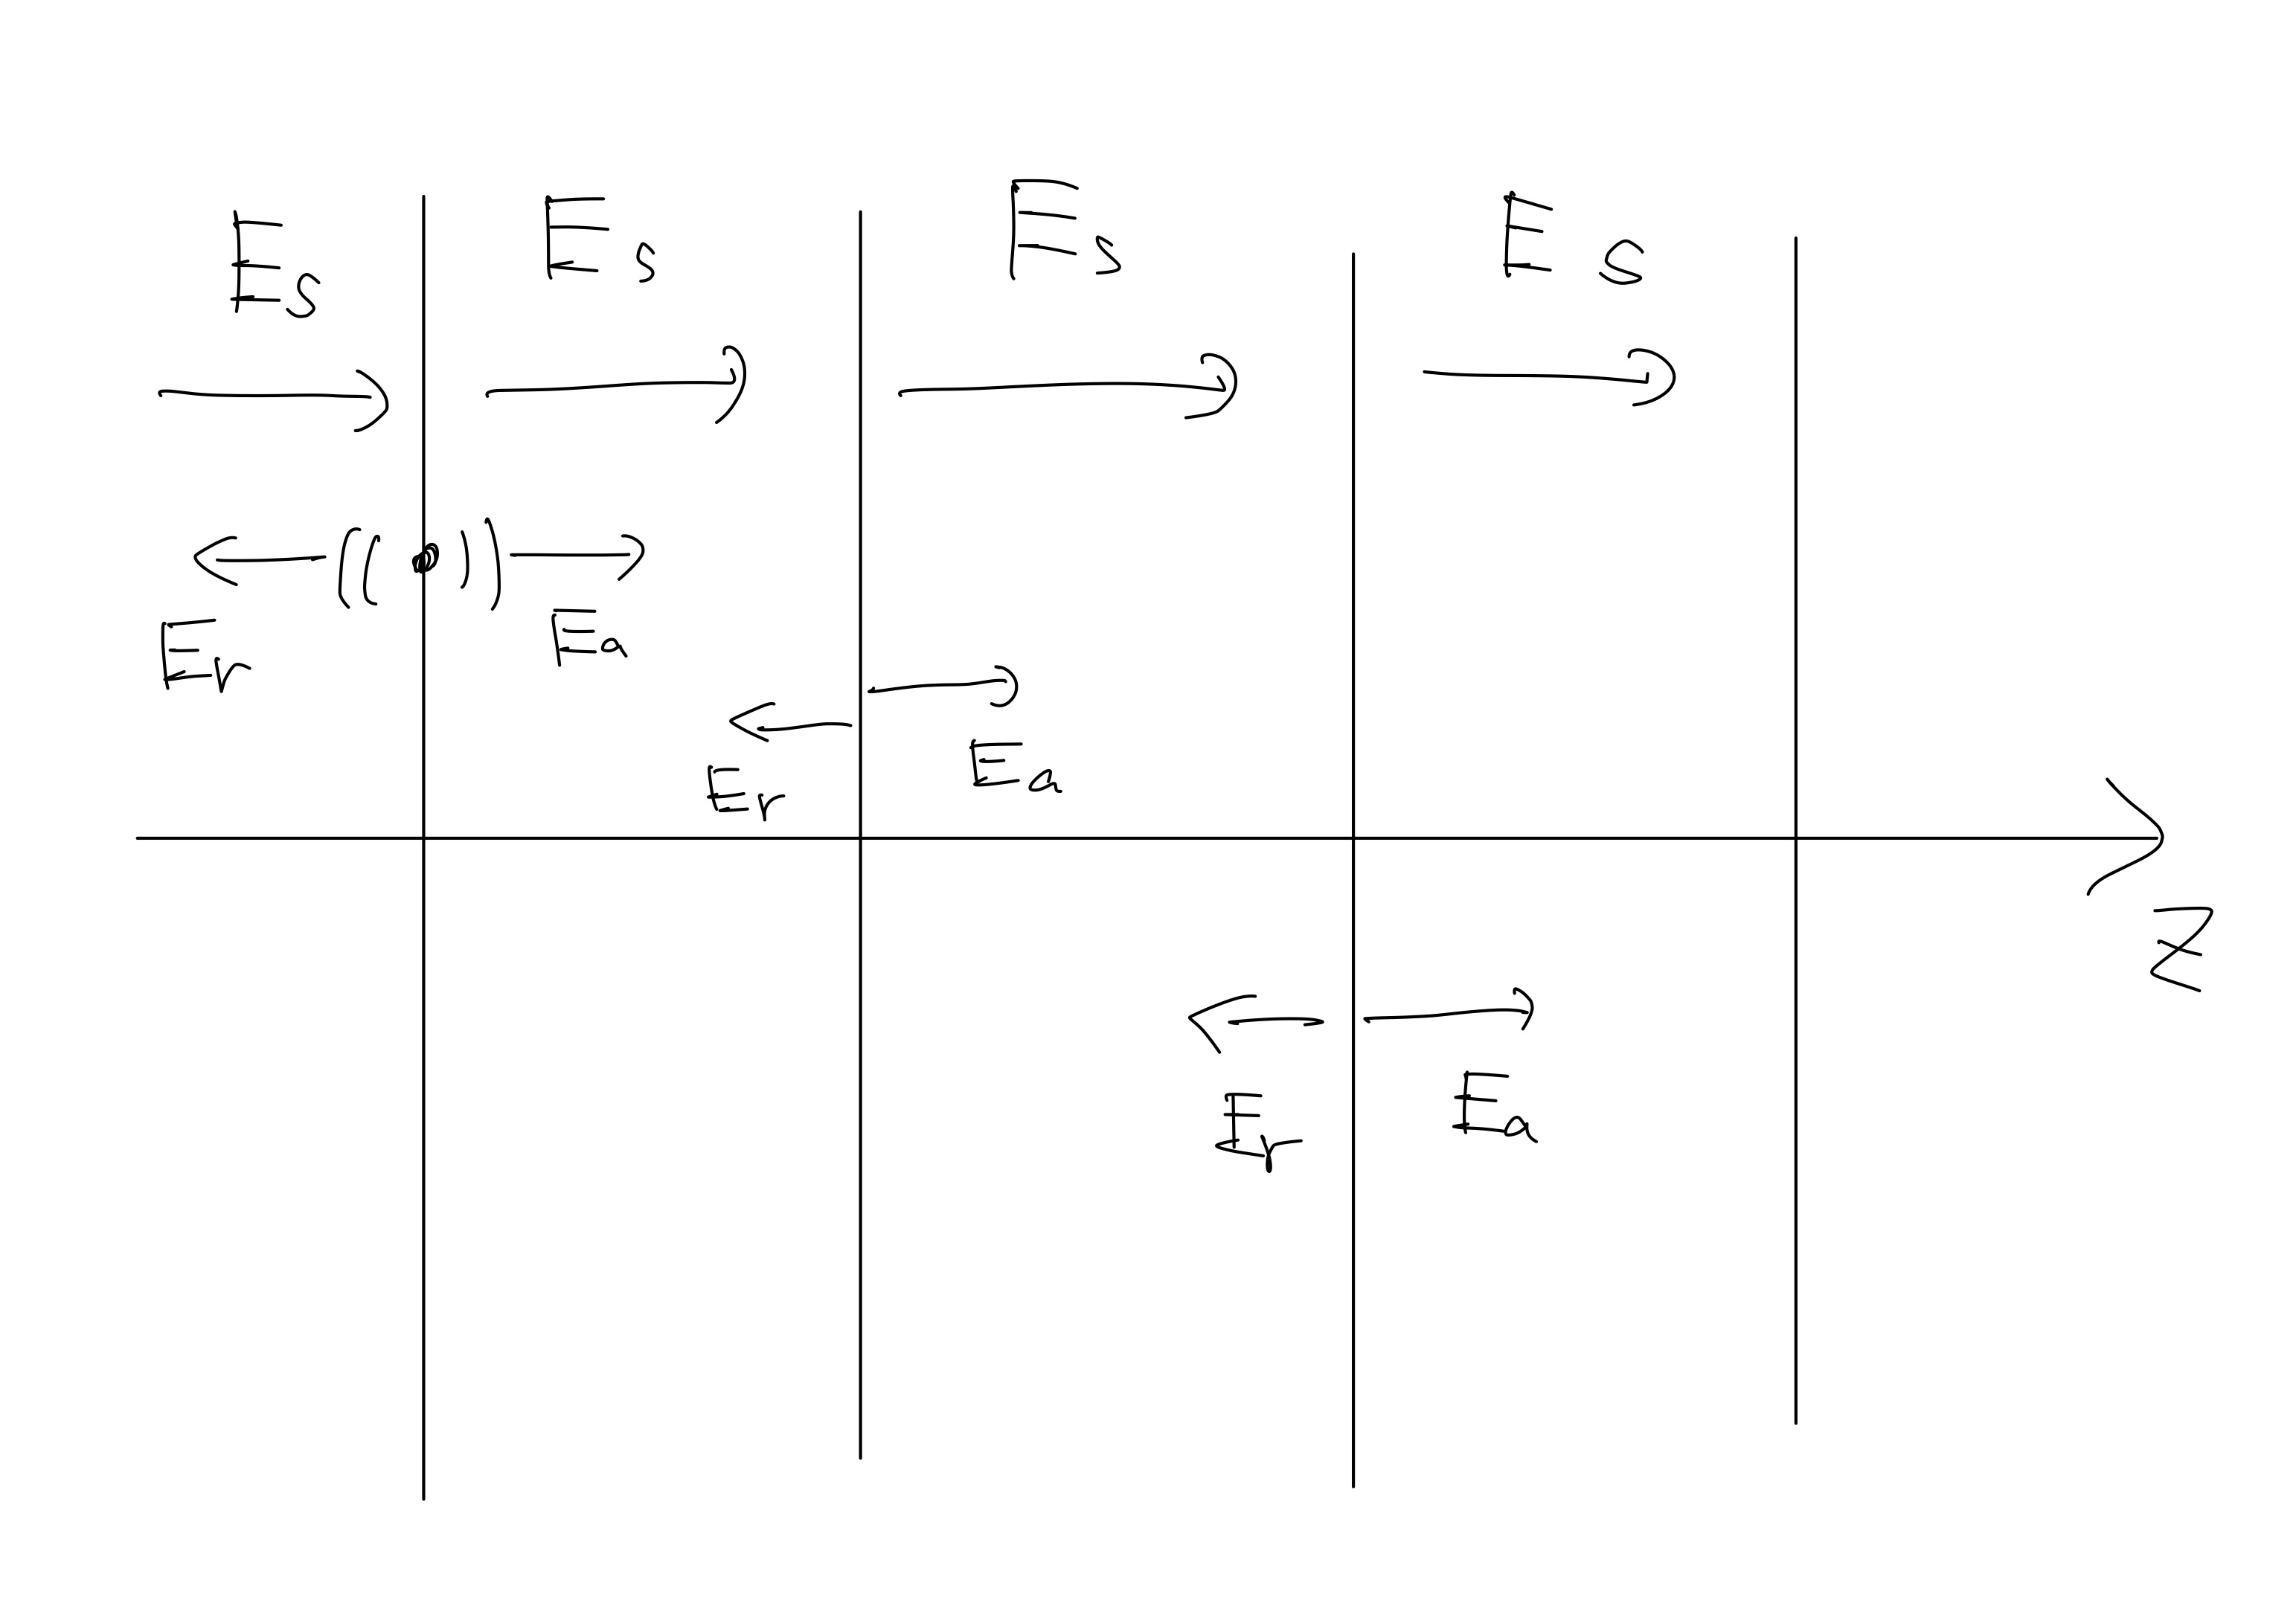
\includegraphics[width=0.5\textwidth]{fig3/Fig-8.jpg}
	%\caption{fig3/Fig-8.jpg}
	\label{fig:fig3-Fig-8-jpg}
\end{figure}
\section{物質中の光の伝搬とポラリトン}
\subsection{前sectionの問題点}
透過光を
\begin{equation}
\label{eq:3-1}
\bm{E}=\bm{E}_s+\bm{E}_a
.\end{equation}
として$\bm{E}_a$を計算した
。
しかしシートで反射され再び励起される二次光の効果などは取り入れられていない。現実の系はもっと複雑である。
マクロな電場$\bm{E}$と分極$\bm{P}$を考え、Maxwell方程式の力を借りる。

\begin{figure}[H]
	\centering
	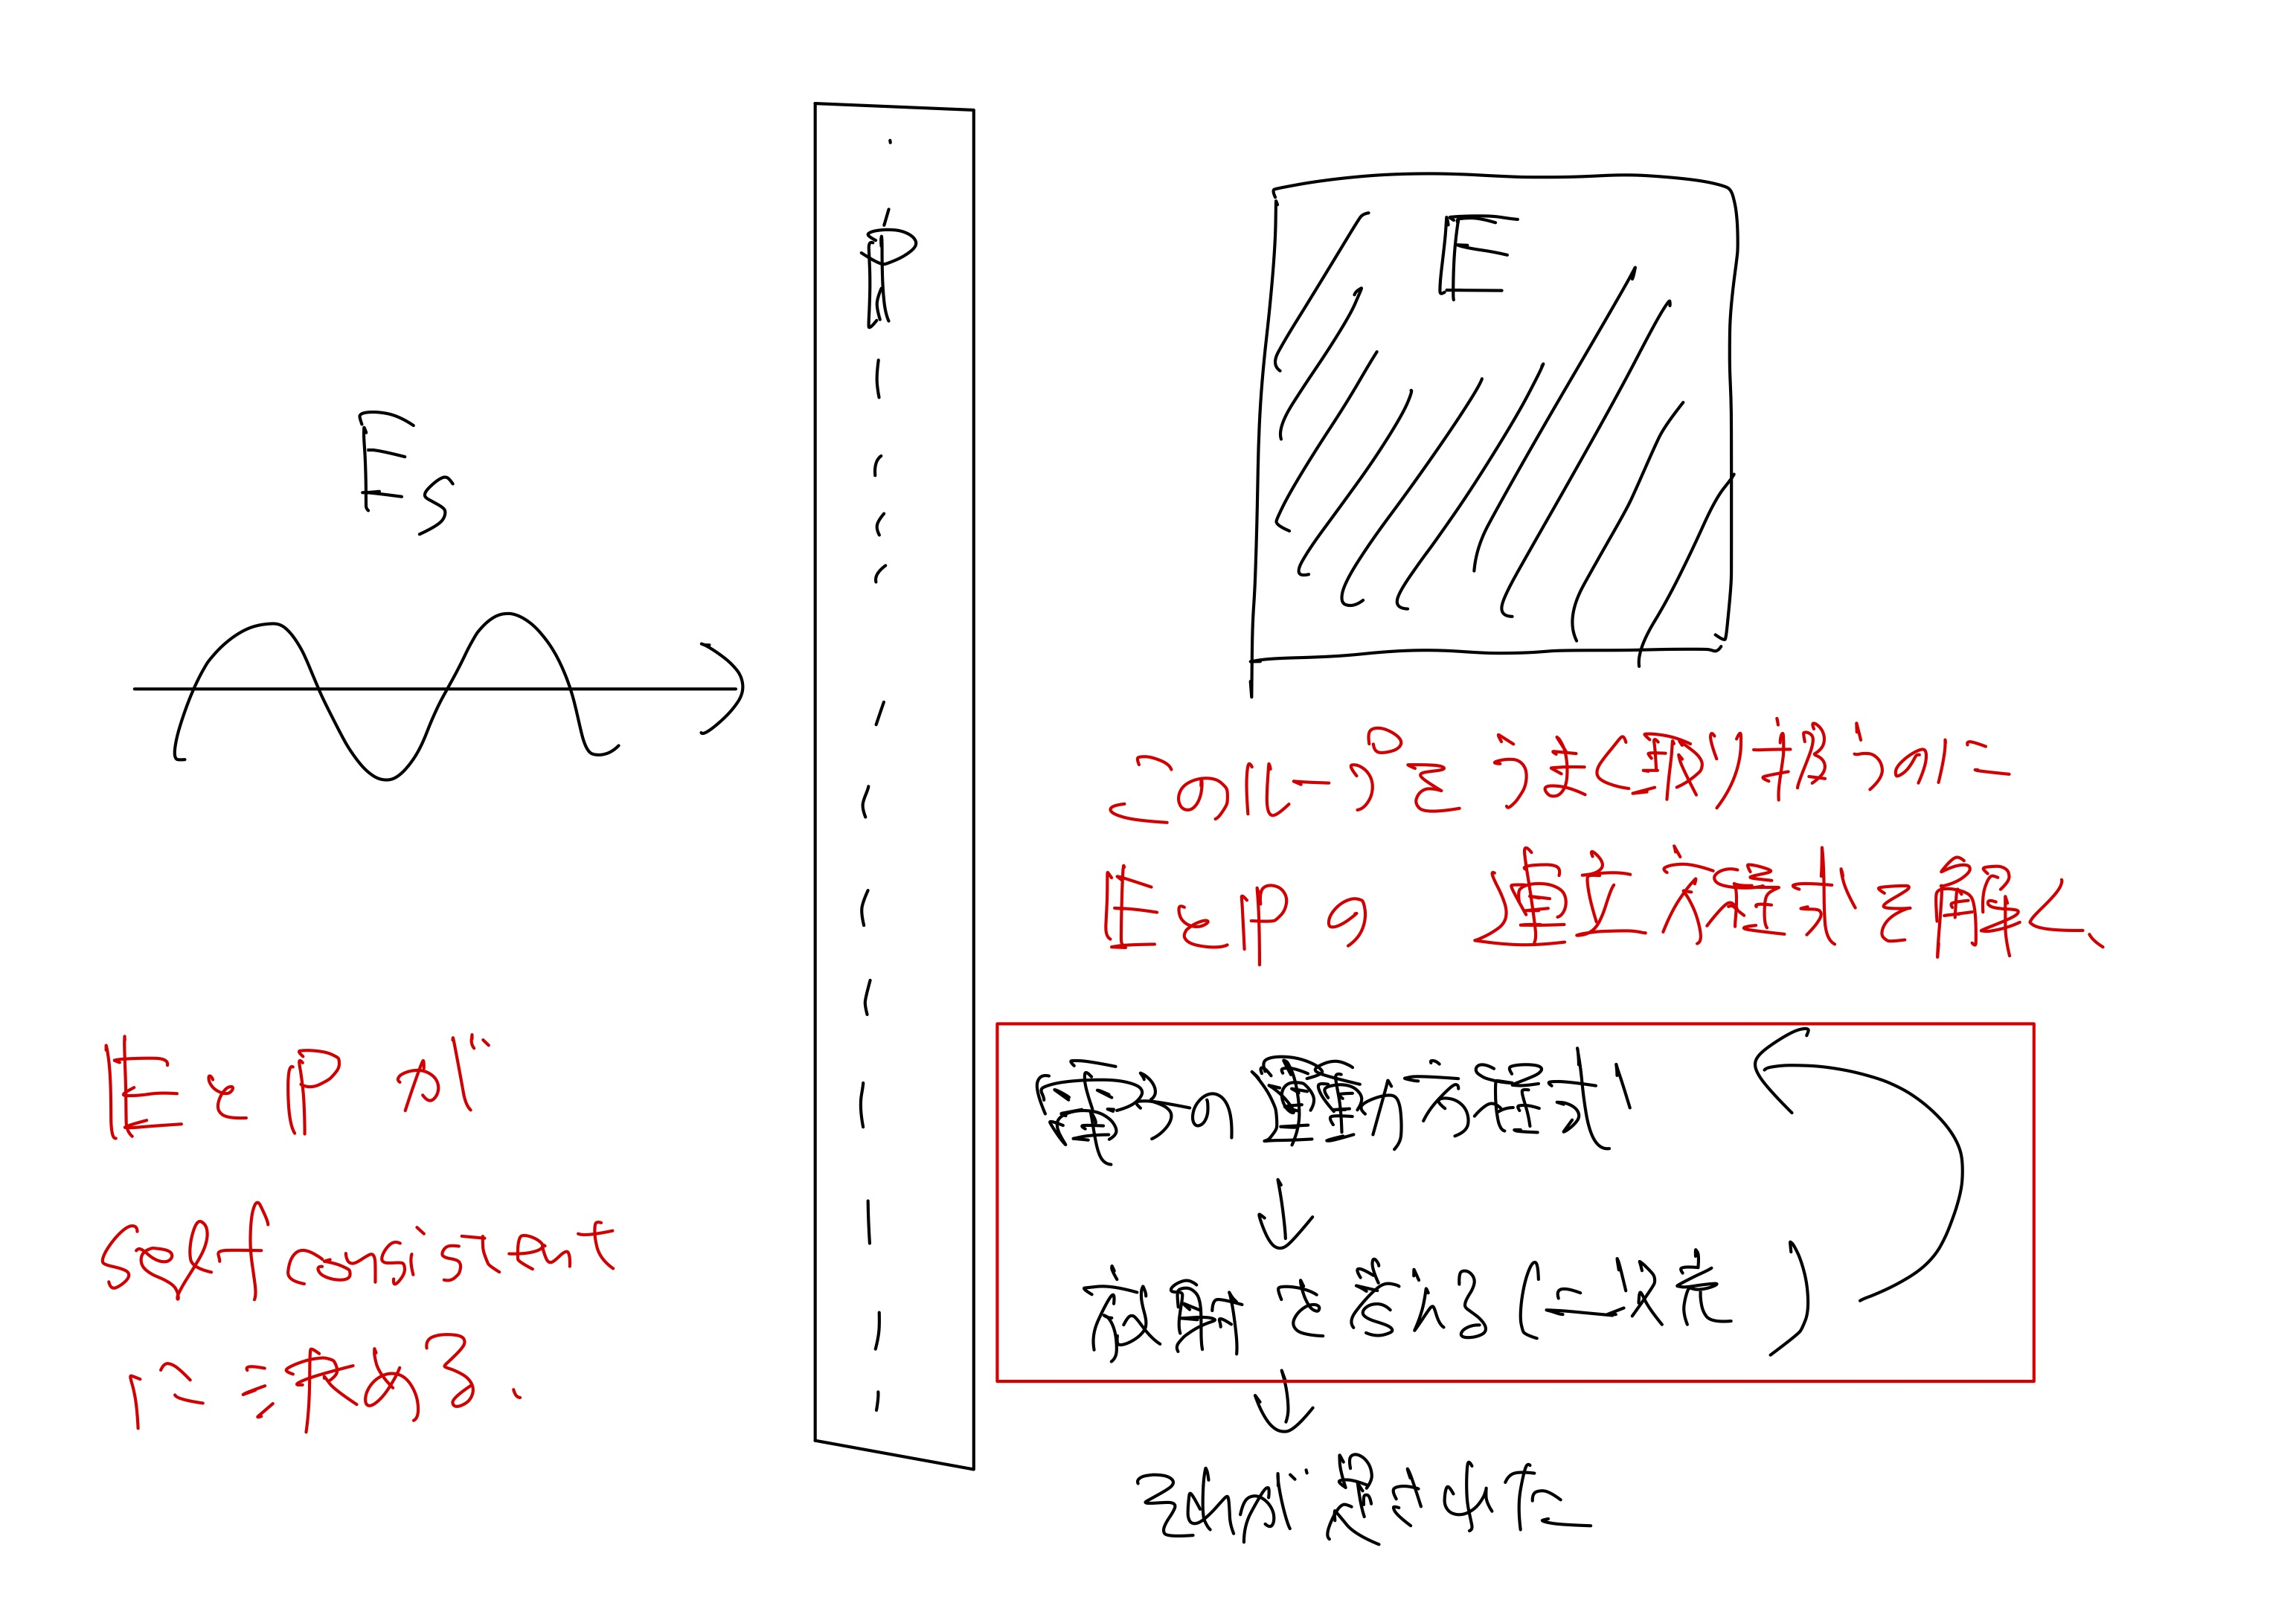
\includegraphics[width=0.5\textwidth]{fig3/Fig-9.jpg}
	%\caption{fig3/Fig-9.jpg}
	\label{fig:fig3-Fig-9-jpg}
\end{figure}
$\bm{E}$ は電磁場であって特徴的な長さは波長$\lambda\sim \SI{1}{\micro m}$である。一方で$\bm{P}$ というのは分極であって特徴的な長さは格子定数$\sim \SI{1}{\angstrom}$で全然違う。
そこで$\bm{P}$ を平均化する.

\begin{figure}[H]
	\centering
	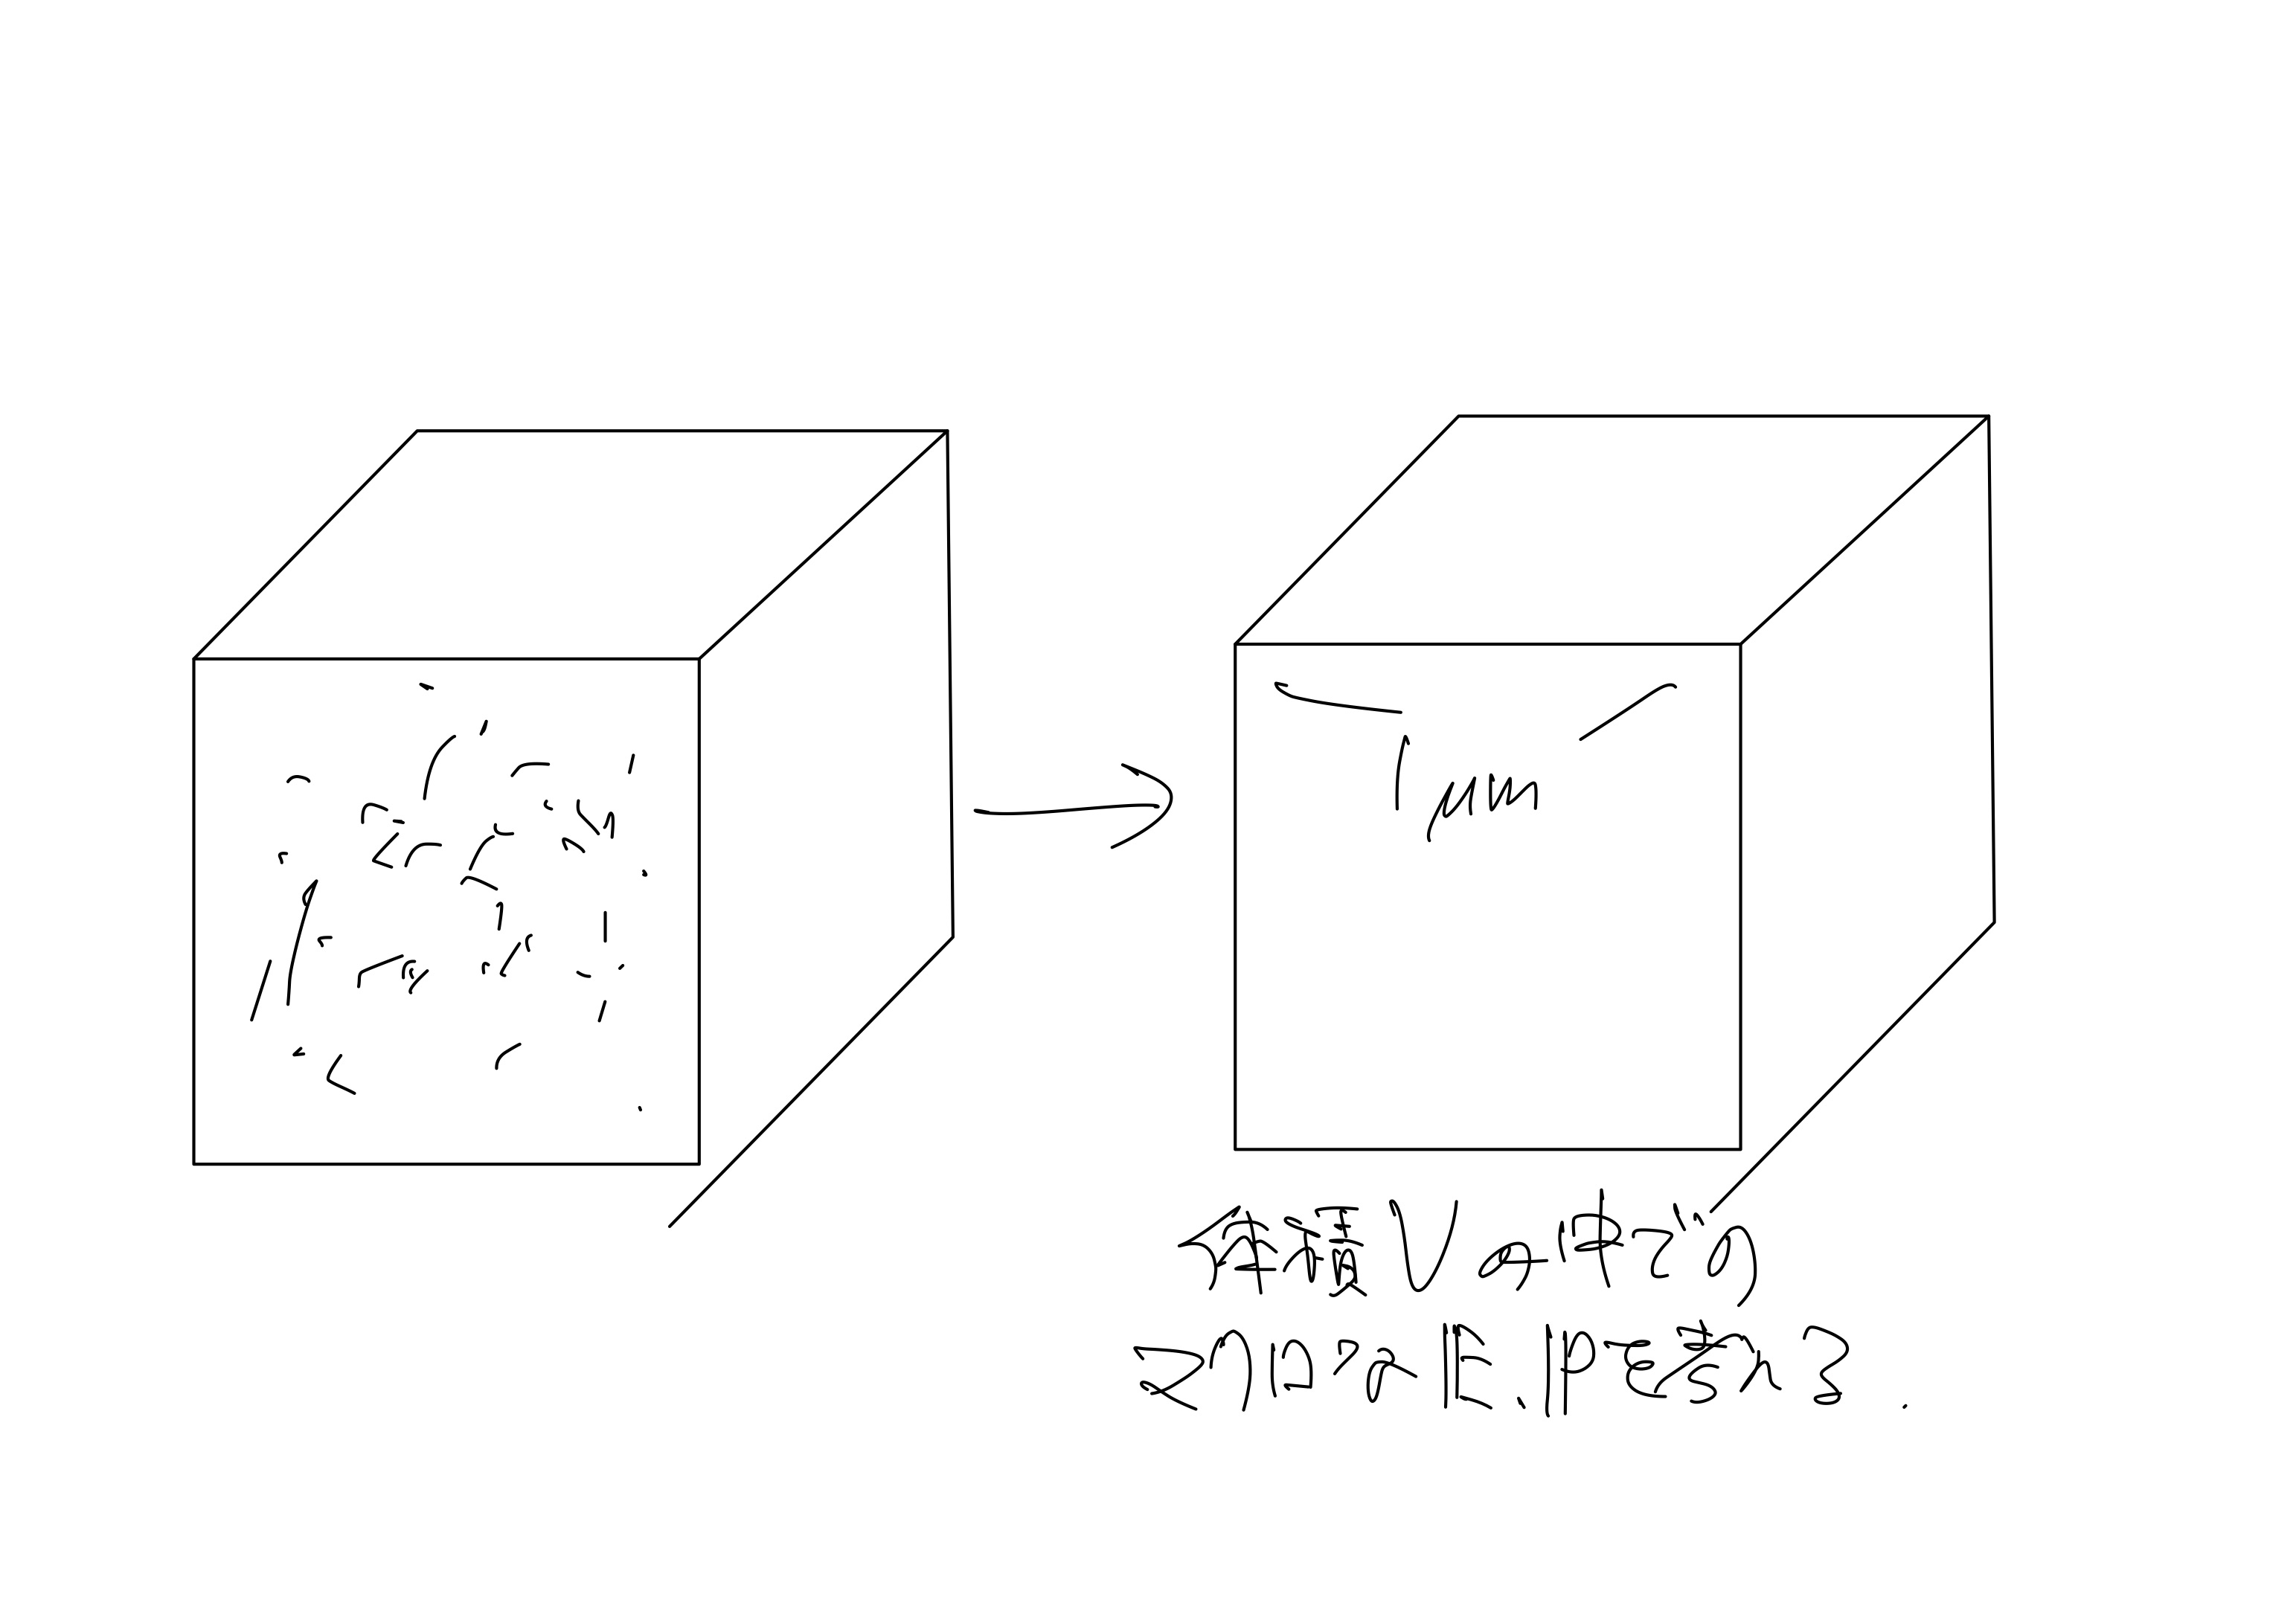
\includegraphics[width=0.5\textwidth]{fig3/Fig-10.jpg}
	%\caption{fig3/Fig-10.jpg}
	\label{fig:fig3-Fig-10-jpg}
\end{figure}
\begin{tcolorbox}[colback=green!10!white]
$\bm{E}$は\textcolor{red}{入射光とすべての二次光を全部足し合わせた}電場の平均($E_s$ だけではない)

$\bm{P}$は体積$V$ 内のすべての双極子モーメントの平均
\begin{equation}
\label{eq:3-2'}
	\bm{P}=\frac{\sum_{i}^{} \mu_i}{V}
.\end{equation}
\end{tcolorbox}
$\bm{E}$ と$\bm{P}$ の連立方程式を立てる。
\subsection{物質中の運動方程式(EからP)}
単位体積中に原子(のような振動子)が$N_0$ 個あった場合
\begin{equation}
\label{eq:3-2}
\bm{P}=N_0 \bm{\mu}=-N_0e \bm{x}
.\end{equation}
したがって\eqref{eq:2-3}は
\[
\bm{x}=-\frac{\bm{P}}{N_0e}
.\] 
とおいて
\begin{equation}
\label{eq:3-3}
	m\left( \frac{d^2}{dt^2}\bm{P}+2\gamma \frac{d}{dt}\bm{P}+\omega^2_0 \bm{P} \right) =N_0e^2\bm{E}
.\end{equation}
とかける。
\begin{tcolorbox}[colback=green!10!white]
分極の方程式は
\begin{equation}
\label{eq:3-4}
\left( \frac{d^2}{dt^2}+2\gamma \frac{d}{dt}+\omega_0^2 \right) \bm{P}=\frac{N_0e^2}{m}\bm{E}
.\end{equation}
\end{tcolorbox}
ただし\eqref{eq:3-4}式の$\bm{E}$ は二次光を含んだ\textcolor{red}{すべての電場の平均であり入射電場$E_s$ではない}。
\[
	\bm{E}=\tilde{\bm{E}}(\omega)e^{-i\omega t}
.\] 
\[
	\bm{P}=\tilde{\bm{P}}(\omega)e^{-i\omega t}
.\] 
とおいたとき
\[
	(-\omega^2-2i\omega\gamma+\omega_0^2)\tilde{\bm{P}}(\omega)=\frac{N_0e}{m}\tilde{\bm{E}}(\omega)
.\] 
したがって
\begin{equation}
\label{eq:3-5}
\tilde{\bm{P}}(\omega)=\frac{N_0e}{m}\times \frac{1}{\omega_0^2-\omega^2-2i\omega\gamma}\tilde{\bm{E}}(\omega):=\varepsilon_0 \tilde{\chi}(\omega)\tilde{\bm{E}}(\omega)
.\end{equation}
ここで$\varepsilon_0$ は真空の誘電率、$\tilde{\chi}(\omega)$ は電気感受率という。

一般に$\tilde{\bm{P}}$が $\tilde{\bm{E}}$に比例するときに成立する光学を\textcolor{red}{線形光学}と呼ぶ

$\tilde{\bm{E}}(\omega)$ が大きすぎると線形近似が成り立たなくなる。これが\textcolor{red}{非線型光学}。
\end{document}
